\documentclass[a4paper, 12pt]{ctexart} % A4幅面，基础字号12pt

% ------------------- 宏包设置 -------------------
\makeatletter
\renewcommand\@cite[2]{\textsuperscript{[#1\if@tempswa , #2\fi]}}
\makeatother
\usepackage[super]{natbib} % 让引用为上标格式
% 第一条：上下左右各留出至少2.5厘米的页边距
\usepackage[margin=2.5cm]{geometry} 
\usepackage{amsmath, amssymb, amsfonts} % 数学宏包
\usepackage{graphicx} % 插入图片
\usepackage{float} % 图片表格浮动位置控制
\usepackage{booktabs} % 三线表
\usepackage{fancyhdr} % 页眉页脚设置
\usepackage{listings} % 代码高亮
\usepackage{xcolor} % 颜色宏包
\usepackage{hyperref} % 超链接
\usepackage{setspace} % 用于调整全局行距
\usepackage{enumitem} % 用于控制列表（itemize/enumerate）的间距，让排版更紧凑
\setlist[itemize]{itemsep=0.15em, topsep=0.2em, parsep=0pt, partopsep=0pt}
\setlist[enumerate]{itemsep=0.15em, topsep=0.2em, parsep=0pt, partopsep=0pt}
\usepackage{dirtree} % 用于绘制专业的文件目录树
\usepackage{tikz}
\usepackage{tabularx}  % 用于创建自动调整列宽的表格
\usepackage{subcaption} % 必须引用这个宏包来支持子图
\usetikzlibrary{shapes.geometric, arrows.meta, positioning}
\usepackage{caption}
\captionsetup{justification=centering} % 标题居中
\usepackage{titlesec}
\usepackage{array}
\usepackage[utf8]{inputenc}
\titleformat*{\section}{\large\bfseries} % 将标题改为 large 尺寸并加粗
\titleformat*{\subsection}{\normalsize\bfseries} % 设置二级标题为标准大小并加粗
\hypersetup{colorlinks=true, linkcolor=black, urlcolor=blue, citecolor=black}
\newcolumntype{Y}{>{\centering\arraybackslash}X} % 定义新的列类型 Y，内容居中且自动调整宽度
% ------------------- 代码格式设置 -------------------
\lstset{
    basicstyle=\ttfamily\small,
    breaklines=true,
    frame=single,
    numbers=left,
    numberstyle=\tiny\color{gray},
    keywordstyle=\color{blue},
    commentstyle=\color{green!50!black},
    stringstyle=\color{red},
    showstringspaces=false
}

% ------------------- 标题与段落间距设置 -------------------
\ctexset{
    section = {
        format = \Large\bfseries,
        name = {,.\ },
        number = \arabic{section},
    },
    subsection = {
        format = \large\bfseries,
        number = \arabic{section}.\arabic{subsection},
    }
}

\setlength{\parskip}{0.4em} % 段间距

% ------------------- 页眉页脚设置 -------------------
\pagestyle{plain}
\fancyhf{}
% 第二条：页码位于页脚中部，用阿拉伯数字
\fancyfoot[C]{\thepage}
\renewcommand{\headrulewidth}{0pt}

\begin{document}
\setstretch{1.25} % 行距 1.25 倍

% ==================== 第一页：承诺书 ====================
\begin{titlepage}
\thispagestyle{empty} % 第一页不显示页码

\begin{center}
    {\small 2026 年北京理工大学数学建模竞赛}\\[1.5cm]
    {\LARGE \bfseries 参赛承诺书}\\[1.5cm]
\end{center}

\noindent\textbf{提交包含此承诺书的 pdf 文件，表明所有此文件的作者共同承诺：}

我们完全清楚，在竞赛开始后参赛队员不能以任何方式，包括电话、电子邮件、“贴吧”、QQ 群、微信群等，与队外的任何人（包括指导教师）交流、讨论与赛题有关的问题；无论主动参与讨论还是被动接收讨论信息都是严重违反竞赛纪律的行为。

\textbf{我们以中国大学生名誉和诚信郑重承诺，严格遵守竞赛章程和参赛规则，以保证竞赛的公正、公平性。如有违反竞赛章程和参赛规则的行为，我们将受到严肃处理。}

我们授权北京理工大学数学建模竞赛组织方，可将我们的论文以任何形式进行公开展示（包括进行网上公示，在书籍、期刊和其他媒体进行正式或非正式发表等）。

\begin{flushright}
2026.5
\end{flushright}

\end{titlepage}

% ==================== 第二页：摘要专用页 ====================
\newpage
% 论文从此页开始编写页码，从“1”开始连续编号
\setcounter{page}{1} 
\thispagestyle{plain}

\begin{center}
    {\small 2026 年北京理工大学数学建模竞赛}\\[1cm]
    {\Large \bfseries 基于 BiLSTM-XGBoost 级联融合的空气质量预测模型}\\[1cm] 
\end{center}

% 在这里添加这一行，专门控制“摘要”二字的字号
\renewcommand{\abstractname}{\Large 摘要}

\begin{abstract}
随着城市化进程推进，空气质量监测与精准预测对校园公共卫生决策变得尤为重要。本文针对北京房山良乡校区2026年第一季度的空气质量监测数据，深入探究了温湿气象因子与六种核心污染物（$\text{PM}_{2.5}, \text{PM}_{10}, \text{O}_3, \text{NO}_2, \text{SO}_2, \text{CO}$）之间的演化规律，构建了高精度的协同预测模型与校园健康生活决策矩阵。

针对问题一，本文首先对原始数据进行物理常识约束清洗与时间连续性插值，并引入正余弦编码、滞后特征（Lag Features）及滑动窗口特征提取时间与气象的潜在关联。通过 \textbf{Spearman 秩相关分析} 揭示了污染物间的“同步富集”与“光化学滴定”效应。
建模时我们发现，$\text{O}_3$ 浓度与温度呈显著的倒“U”型非线性响应，而 $\text{CO}$ 等一次污染物则表现出明显的“热力清除”特征。
最后我们还利用互相关分析定量评估了温湿影响的滞后效应，发现颗粒物受气象驱动具有显著的惯性积累。

针对问题二，为捕捉多污染物间的复杂非线性耦合关系，本文提出一种基于 \textbf{Stacking} 策略的 \textbf{BiLSTM-XGBoost 级联融合模型}。
该架构分为两层：第一层利用\textbf{双向长短期记忆网络（BiLSTM）}提取深层时序隐藏特征 $\mathbf{H}_{\text{hidden}}$；
第二层则利用多输出 XGBoost（Multi-Output XGBoost）作为先验知识的修正器与非线性融合器，实现对六种污染物的协同预测。
实验结果显示，模型在测试集上的表现优秀，$\text{SO}_2$ 和 $\text{CO}$ 的决定系数 $R^2$ 均超过 0.98，验证了模型在处理多变量时间序列任务中的鲁棒性。
针对该模型可解释性，本文引入博弈论中的 \textbf{SHAP} 归因分析。在不预设化学反应方程式的前提下，模型自主挖掘出 $\text{NO}_2$ 作为 $\text{PM}_{2.5}$ 关键前体物的催化效应，并定量证实了高温高湿环境下的“吸湿增长”驱动机制。

针对问题三，本文依据国家 AQI 标准建立了空气质量分级模型，并结合校区师生作息规律，构建了包含 AQI 等级、首要污染物、温湿舒适度四个维度的 \textbf{校园健康生活决策矩阵}，为晨跑、体测、全天通风等校园活动提供动态、科学的行动指南。

\bigskip % 增加一点间距

% 3. 每一个关键词都标黑
\noindent \textbf{关键词：} \textbf{空气质量预测}；\textbf{BiLSTM-XGBoost 融合模型}；\textbf{Stacking 集成学习}；\textbf{SHAP 可解释性分析}；\textbf{Spearman 相关分析}；\textbf{滞后特征}

\end{abstract}

\newpage
\tableofcontents
\newpage

% ==================== 第一部分：问题背景 ====================
\section{问题背景}

随着城市化进程的加快和工业化水平的提高，空气质量已成为衡量城市宜居度和公共卫生水平的关键指标。在空气质量评估体系中，PM2.5、PM10、O$_3$、NO$_2$、SO$_2$ 以及 CO 是六项核心污染物指标。这些污染物的浓度不仅取决于污染源的排放强度，还受到气象条件的深度耦合影响。

北京房山良乡地区作为典型的科教新区，其空气质量直接关系到校区内数万名师生的身心健康与日常活动安排。温度与湿度作为基础气象要素，通过物理扩散和化学反应显著改变污染物的时空分布。例如，湿度增加可能导致颗粒物吸湿增长，而温度变化则可能触发逆温现象。值得注意的是，气象因素对污染物的影响往往存在“滞后效应”，即前一时刻的温湿状态可能决定了后续的浓度峰值。

本文基于 2026 年第一季度良乡地区的逐小时监测数据，旨在探讨温湿条件与单一污染物及多污染物协同变化之间的定量关系，建立预测模型并提供科学的空气质量分级指导方案，为校园生活的科学决策提供支撑。

% ==================== 第二部分：问题分析 ====================
\section{问题分析与研究框架}

\subsection{针对问题一的分析：单一污染物与影响因子的关联性研究}
问题一要求分析单一污染物浓度与时间、温度、湿度之间的关系。首先，需对原始数据进行处理，剔除异常值和缺失值。由于空气质量数据具有明显的周期性和季节性，我们将引入时间特征变量。通过使用 Spearman 秩相关分析，定量评估污染物浓度与温度、湿度的线性及非线性相关强度。针对题目中提到的“滞后性”，我们测算了温度和湿度分别对污染物浓度的滞后效应的Spearman 相关系数，为后续的预测模型提供重要的特征工程指导。

\subsection{针对问题二的分析：多污染物协同变化规律的预测建模}
问题二要求建立数学模型预测六种污染物的协同变化。考虑到六种污染物之间并非完全独立，而是存在复杂的耦合关系（如 NO$_2$ 与 O$_3$ 的光化学转化），简单的单变量回归难以捕捉其演化特征。我们拟采用建立 BiLSTM + XGBoost 级联融合模型来描述污染物间的相互作用及其对气象条件的响应。模型将时间、温度、湿度作为外生变量，将六种污染物浓度作为内生变量，通过深度学习架构，捕捉污染物浓度的动态演变规律。

\subsection{针对问题三的分析：空气质量分级与活动建议决策模型}
问题三要求建立空气质量分级预测模型并提供活动指导。分析认为，本问的核心在于将“预测浓度值”转化为“决策建议值”。首先，需参考国家空气质量指数（AQI）计算标准，将六种污染物的预测浓度转换为分指数（IAQI），并确定首要污染物。随后，针对校区学生的特殊性，结合温湿舒适度指数，建立评价矩阵。通过综合评价模型，将空气质量等级与具体活动（如室外体育课、社团活动、室内自习等）进行映射，给出具有针对性的生活指导。

\subsection{研究框架}
基于此，我们的研究框架如图所示
\begin{figure}[htbp]
    \centering
    \hspace*{-1.5cm} % 负值越小，向左移动越多
    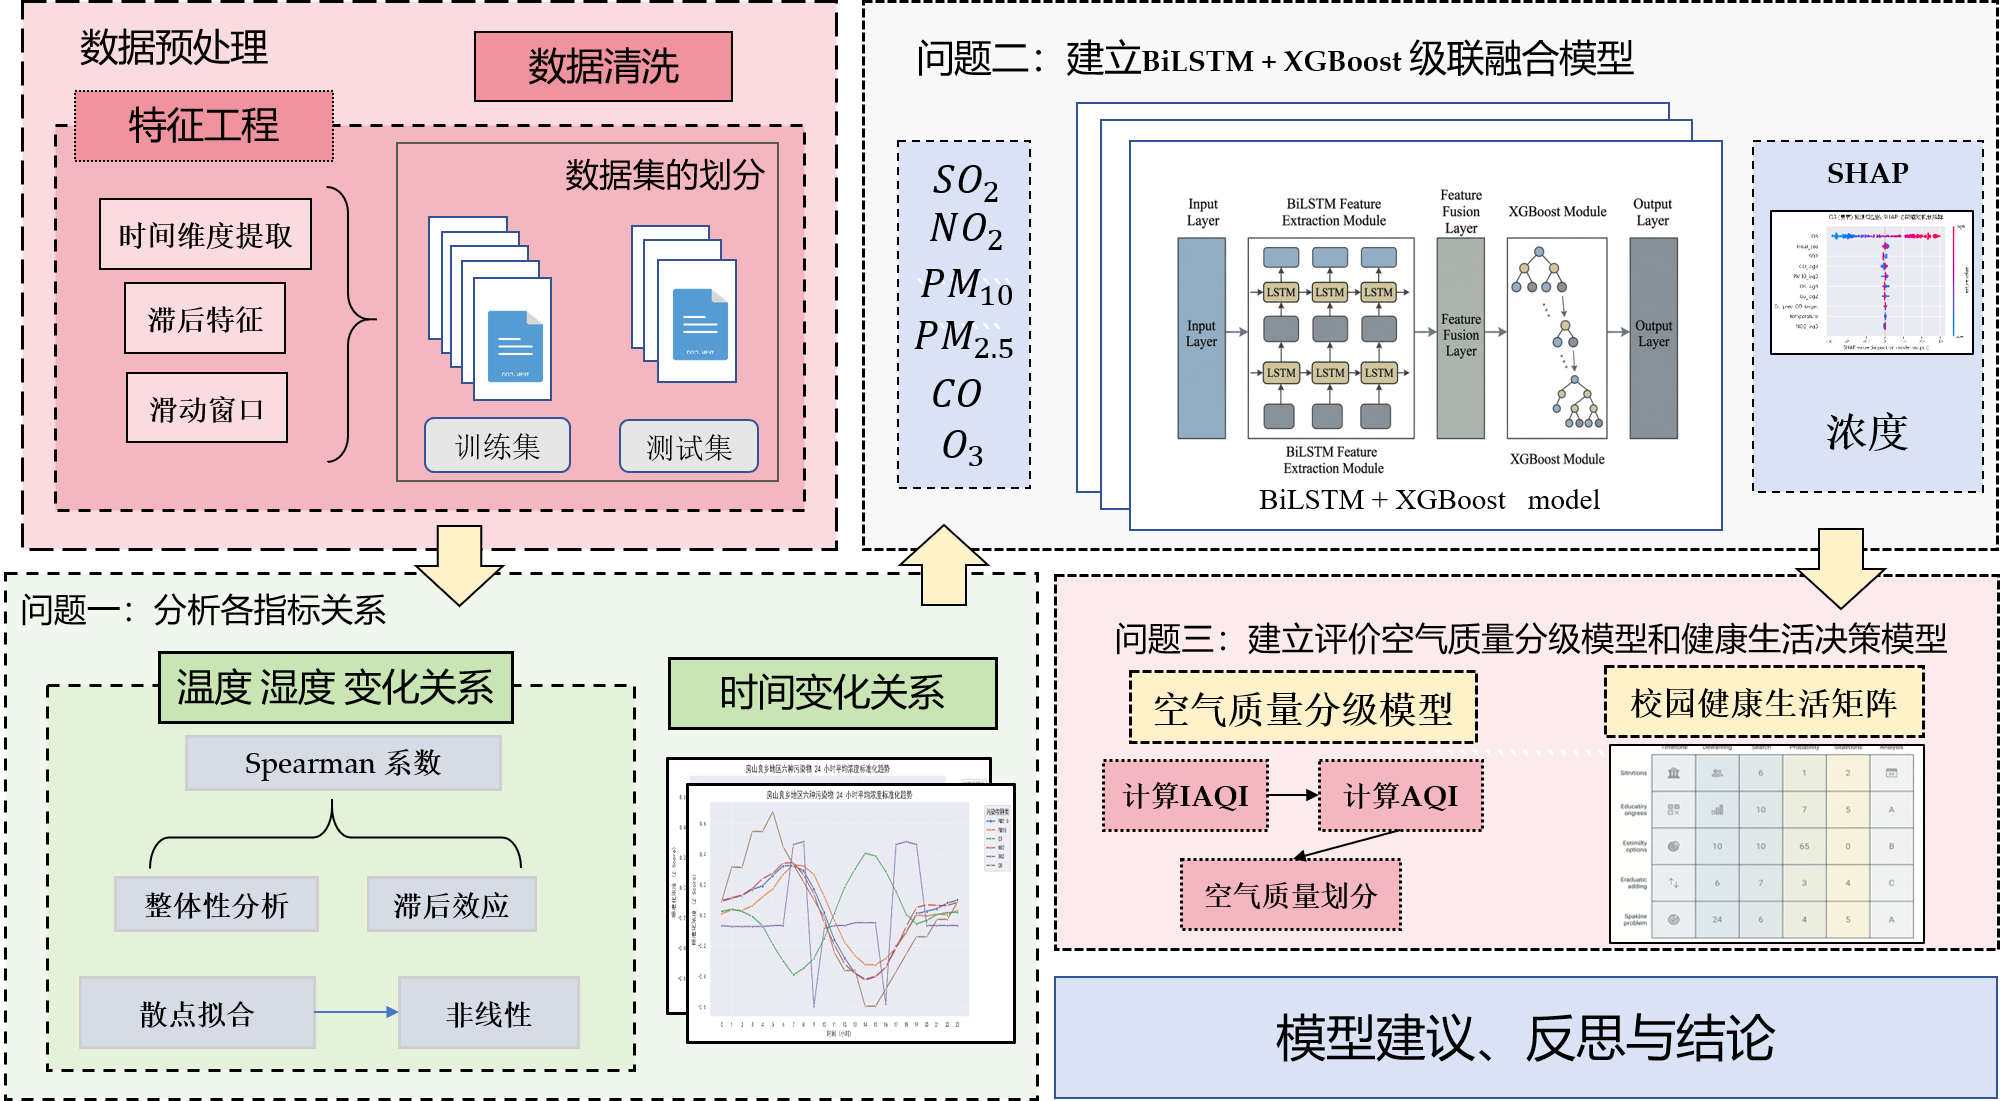
\includegraphics[width=1\textwidth]{images/thinking.png} 
    \caption{研究思路示意图} % 图片下方的标题
    \label{fig:idea} % 用于正文交叉引用的标签
\end{figure}

% ==================== 第三部分：模型假设 ====================
\section{模型假设}
为了简化问题并确保模型的科学性与普适性，本文提出以下合理假设：

\begin{itemize}
    \item \textbf{数据代表性假设：} 假设附件所提供的良乡地区监测站数据准确可靠，能够代表良乡校区整体的空气质量状况；
    \item \textbf{气象主导性假设：} 假设在研究时间段内（2026年1月-3月），当地的大规模工业污染排放源和交通流量相对稳定，污染物浓度的短期波动主要由气象条件和时间特征决定；
    \item \textbf{采样连续性假设：} 假设大气运动在小时尺度内是连续变化的，忽略瞬时极端突发环境事件对数据的影响；
    \item \textbf{环境一致性假设：} 在分析温湿度影响时，假设其他未给出的气象因素（如风速、风向、气压等）对模型整体趋势的影响包含在随机误差项中，或与温湿度具有较强的共线性。
\end{itemize}

% ==================== 第四部分：模型建立 ====================
\section{模型建立}

\subsection{数据预处理}
原始空气质量监测数据在采集和传输过程中，往往会受到仪器校准偏差、环境突变、传输中断等因素的干扰。此外，单一的瞬时浓度无法全面反映污染物的演化规律。因此，在建立预测模型前，我们需要对数据进行了严格的异常值清洗、时序插值、特征工程构建以及标准化处理，以提高模型的预测精度。

\subsubsection{异常值检测与数据清洗}

\textbf{（1）物理常识约束与异常值剔除}

首先，将数据集的字符串格式时间转化为时间戳序列，并将其设置为数据的索引，以保证时序分析的连续性。针对空气污染物的物理特性，任何污染物的浓度值不可能小于零，同时相对湿度必须介于 $0\% \sim 100\%$ 之间。因此，我们对违反物理常识的监测值进行剔除，将其标记为缺失值（NaN）。

\textbf{（2）时间序列连续性插值填补}

为保证气象和污染物随时间演变的连续性，避免后续提取滞后特征时出现截断，我们采用基于时间顺序的线性插值法（Time Interpolation）对前两步产生的缺失值进行填补，重构出完整、平滑的时间序列数据。
\bigskip
\subsubsection{特征提取工程}


\textbf{（1）时间周期维度与人类活动特征提取}\cite{fan2012}

空气污染受人类社会活动和太阳光照的周期性影响显著。我们将时间戳进行拆解，构建了以下关键替代特征：一是提取“小时 (0-23)”以捕捉早晚高峰的汽车尾气排放规律及午后光化学反应特征；二是构建“是否供暖 (0/1)”特征（以3月15日为分界线），来量化冬季燃煤供暖对 PM2.5 和 SO$_2$ 的增量影响。

传统的小时特征（0-23）在数值上存在 23 点与 0 点不连续的问题。为此，我们引入正余弦编码（Sine/Cosine Encoding），将小时特征映射至二维连续的单位圆空间，其计算公式为：

\begin{equation}
    Hour_{sin} = \sin\left(\frac{2\pi \cdot t}{24}\right), \quad Hour_{cos} = \cos\left(\frac{2\pi \cdot t}{24}\right)
\end{equation}

该编码方式能够有效保留时间的循环特性，帮助模型识别日周期波动规律。

\textbf{（2）气象条件与污染物的滞后特征（Lag Features）}

空气质量的变化不仅取决于当前时刻的温湿度，更受到过去环境状态的影响。为捕捉大气系统的“记忆性”和污染扩散的“滞后性”，我们引入了自回归思想。针对温度、湿度以及六种污染物，分别向历史时刻回溯，构造了滞后 1 小时、2 小时、3 小时的特征序列（ $X_{t-1}, X_{t-2}, X_{t-3}$），从而让模型能够学习到污染物的累积与消散惯性。

\textbf{（3）气象状态的滑动窗口特征（Rolling Windows）}

为了弱化瞬时气象波动带来的噪声，更好地反映大气边界层的整体稳定度，我们构建了滑动窗口统计特征。具体包括过去 3 小时的平均温度与平均湿度，以及过去 6 小时内的最大温差（最高温与最低温之差）。最大温差能够有效辅助模型判断近地面逆温层的破坏或形成情况。

\subsubsection{数据归一化与数据集划分}

\textbf{（1）预测目标的有监督转化}

为了使时间序列预测任务能够应用监督学习算法，本文采用 $Shift(-1)$ 策略构建了“预测 Label”。数学表达如下：
$$ Target_{t} = X_{t+1} $$
其中，$Target_{t}$ 为模型在 $t$ 时刻需要拟合的目标值，$X_{t+1}$ 为该污染物在未来一小时的实际浓度。

\textbf{（2）无效数据截断}

在进行时序滑动（Shift）和滚动计算（Rolling）时，时间序列的前几个小时会不可避免地产生边界空值。考虑到原始数据量充足（两千余条观测记录），我们直接将前 3-6 行因特征构造产生的空值行剔除。


\textbf{（3）训练集与测试集划分}

为客观评估预测模型的泛化能力，避免时间序列数据的信息泄露（Data Leakage），我们严格按照时间先后顺序进行数据集划分。选取 2026 年 1 月 1 日至 3 月 15 日的数据作为训练集，3 月 16 日至 3 月 31 日的数据作为测试集，以此验证模型对未来未知时段的空气质量预测效能。


% ==================== 第四部分：问题一模型建立 ====================
\subsection{问题一：单一污染物与影响因子的关系分析}

问题一要求探究单一污染物浓度与时间、温度及湿度之间的定量关系。我们首先通过统计分析挖掘污染物在日周期尺度上的演化规律，随后结合气象学原理分析温湿度对不同污染物的物理/化学驱动机制。

\subsubsection{Z-score 标准化归一化}
为了消除不同污染物浓度量纲和数量级的差异（例如 CO 浓度通常在 0.5-2 之间，而 PM10 浓度可高达 150 以上，温度则存在负值），使它们在统一尺度上进行比较和可视化，本研究采用了 Z-score 标准化方法对原始数据进行了预处理。对于任意一个数据点 $x$，其标准化后的值 $z$ 通过以下公式计算：
\begin{equation}
    x_{norm} = \frac{x - \mu}{\sigma}
\end{equation}
其中，$\mu$ 为该特征样本的均值，$\sigma$ 为标准差。此操作在消除量纲影响的同时保留了数据的原始分布形态。

\subsubsection{污染物浓度随时间变化的规律分析}
在本研究中，我们对六种主要污染物（PM2.5、PM10、O3、NO2、SO2、CO）分别进行了Z-score标准化，并基于标准化后的数据绘制了24小时平均浓度趋势图。
同时，我们还绘制了六种污染物的24小时浓度日变化图，以更直观地展示它们在一天内的动态演变规律。
% --- 将这段代码插入到你想显示图片的地方 ---
\begin{figure}[h]
    \centering
    % width=0.8\textwidth 表示图片宽度占页面正文宽度的 80%
    % 大括号里填你的图片文件名，不需要写后缀也能识别，但写上更保险
    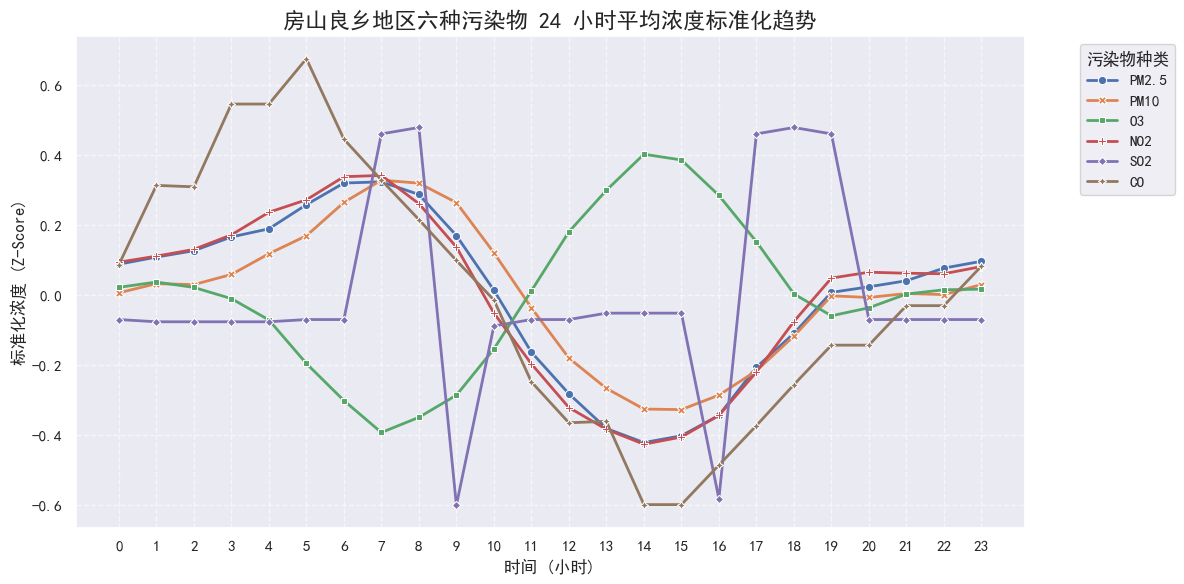
\includegraphics[width=1.0\textwidth]{images/1.png} 
    
    \caption{良乡地区六种污染物 24 小时平均浓度趋势变化图} % 图片下方的标题
    \label{fig:24h_trend} % 用于正文交叉引用的标签
\end{figure}
\begin{figure}[h]
    \centering
    % width=0.8\textwidth 表示图片宽度占页面正文宽度的 80%
    % 大括号里填你的图片文件名，不需要写后缀也能识别，但写上更保险
    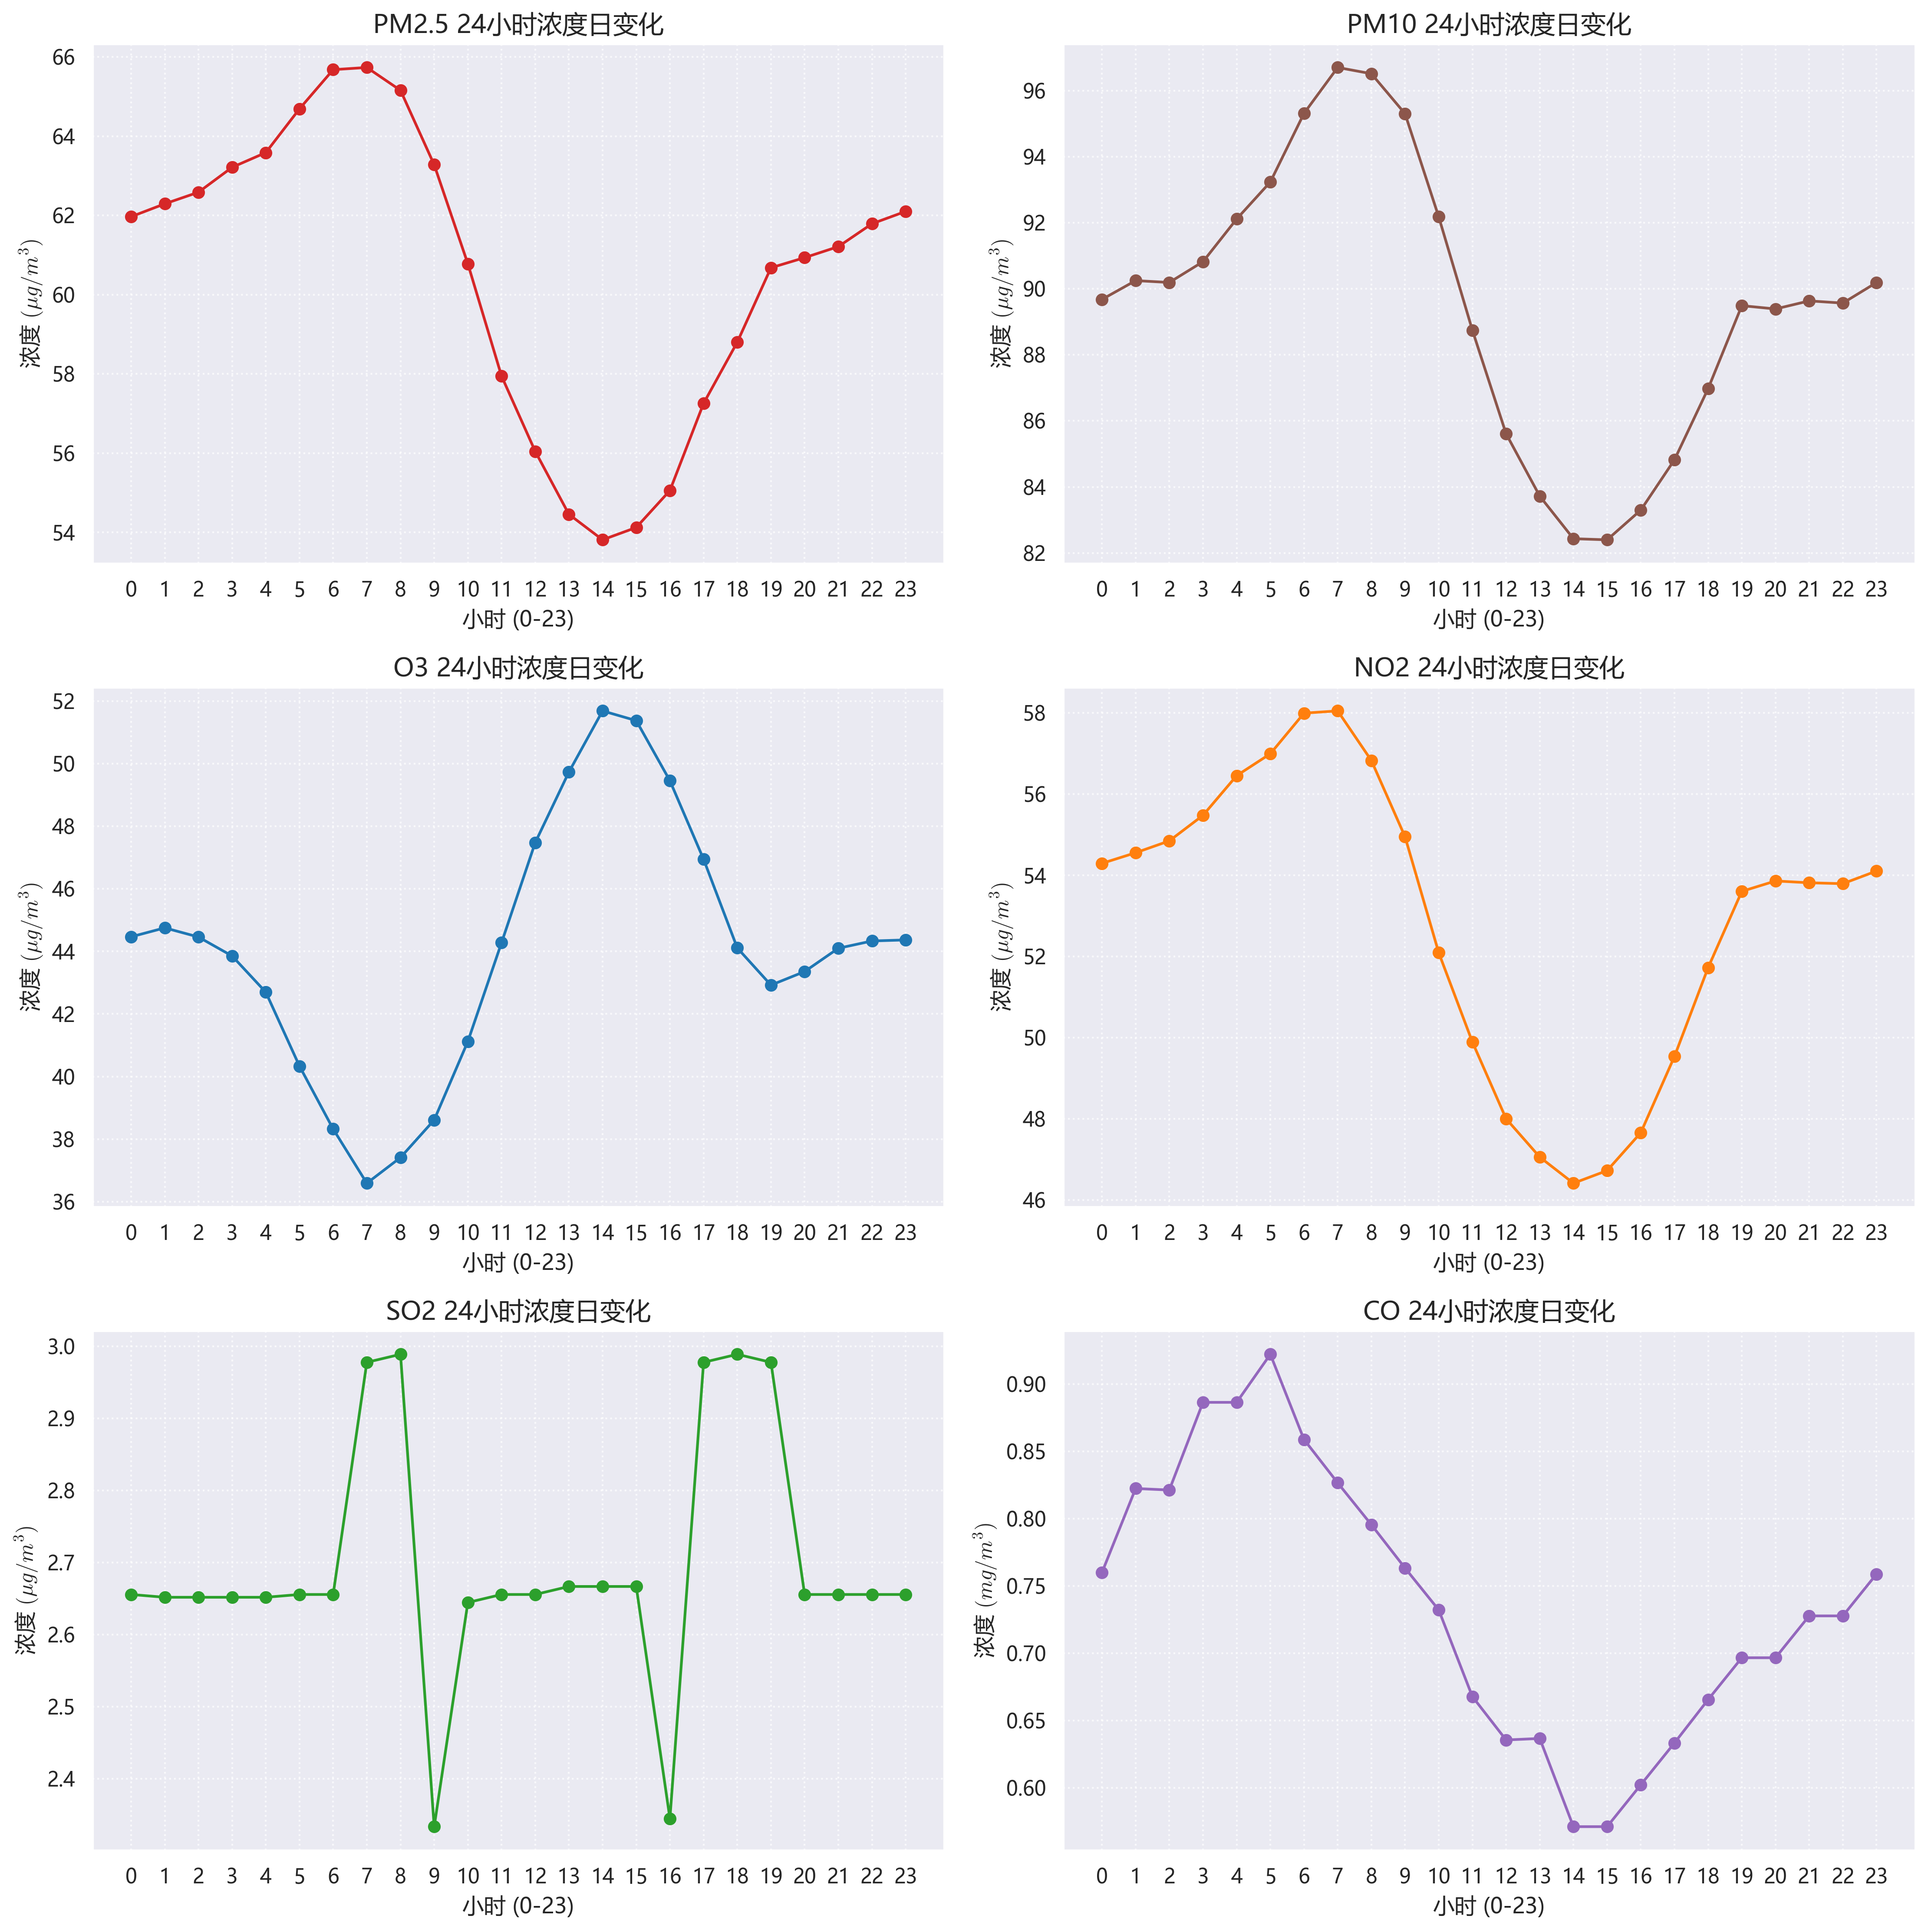
\includegraphics[width=0.8\textwidth]{images/2.png} 
    
    \caption{良乡地区六种污染物 24 小时浓度日变化图} % 图片下方的标题
    \label{fig:24h_daily_trend} % 用于正文交叉引用的标签
\end{figure}
% ---------------------------------------

\textbf{（1）颗粒物与一次气态污染物的“双峰双谷”特征}

从图中不难发现，PM2.5、PM10、NO$_2$、CO 及 SO$_2$ 呈现出显著一致的“双峰双谷”形态。第一个峰值出现在早高峰时段（8:00--10:00），第二个峰值出现在傍晚至深夜（19:00--21:00）；而浓度低谷则出现在午后（14:00--16:00）及凌晨。

\noindent 其成因可归纳为：
\begin{itemize}
    \item \textbf{人类活动规律：} 峰值时段与城市上下班交通高峰高度吻合，机动车尾气排放是 NO$_2$、CO 和一次颗粒物的主要来源 ；
    \item \textbf{大气边界层演化：} 夜间及清晨气温较低，易形成贴地“逆温层”，大气性质极其稳定，导致垂直扩散受阻，污染物在近地面快速累积 。午后随着太阳辐射增强，地表增温，边界层高度抬升，垂直湍流增强，污染物被稀释并向高空扩散，浓度降至全日低谷 。
\end{itemize}

\bigskip
\textbf{（2）臭氧（O$_3$）的“单峰型”反向变化特征}

与上述污染物截然相反，O$_3$ 浓度在午后 14:00--16:00 达到一日内的最高点，而在夜间处于极低水平，呈现明显的“单峰”特征 。

\noindent 这种现象的物理机制在于：
\begin{itemize}
    \item \textbf{光化学反应驱动：} O$_3$ 并非直接排放，而是在太阳紫外辐射下由前体物（NOx 和 VOCs）发生光化学反应生成 。午后阳光最强、气温最高，光化学反应速率达到峰值 ；
    \item \textbf{滴定消耗效应：} 夜间光照消失，光化学反应停止，且机动车持续排放的 NO 会通过“滴定反应”消耗 O$_3$（$NO + O_3 \rightarrow NO_2 + O_2$），使其浓度迅速跌至谷底 。
\end{itemize}




\subsubsection{周变化与月度变化规律}
我们也分析了工作日与周末的污染物浓度差异，以及不同月份之间的变化趋势。通常情况下，城市中的“周末效应”会导致工作日的污染物浓度高于周末，主要原因是工作日交通和工业活动更为频繁。

然而，在良乡地区，我们并未观察到显著的“周末效应”，这可能与该区域的地理位置和人类活动模式有关。

\begin{figure}[h]
    \centering
    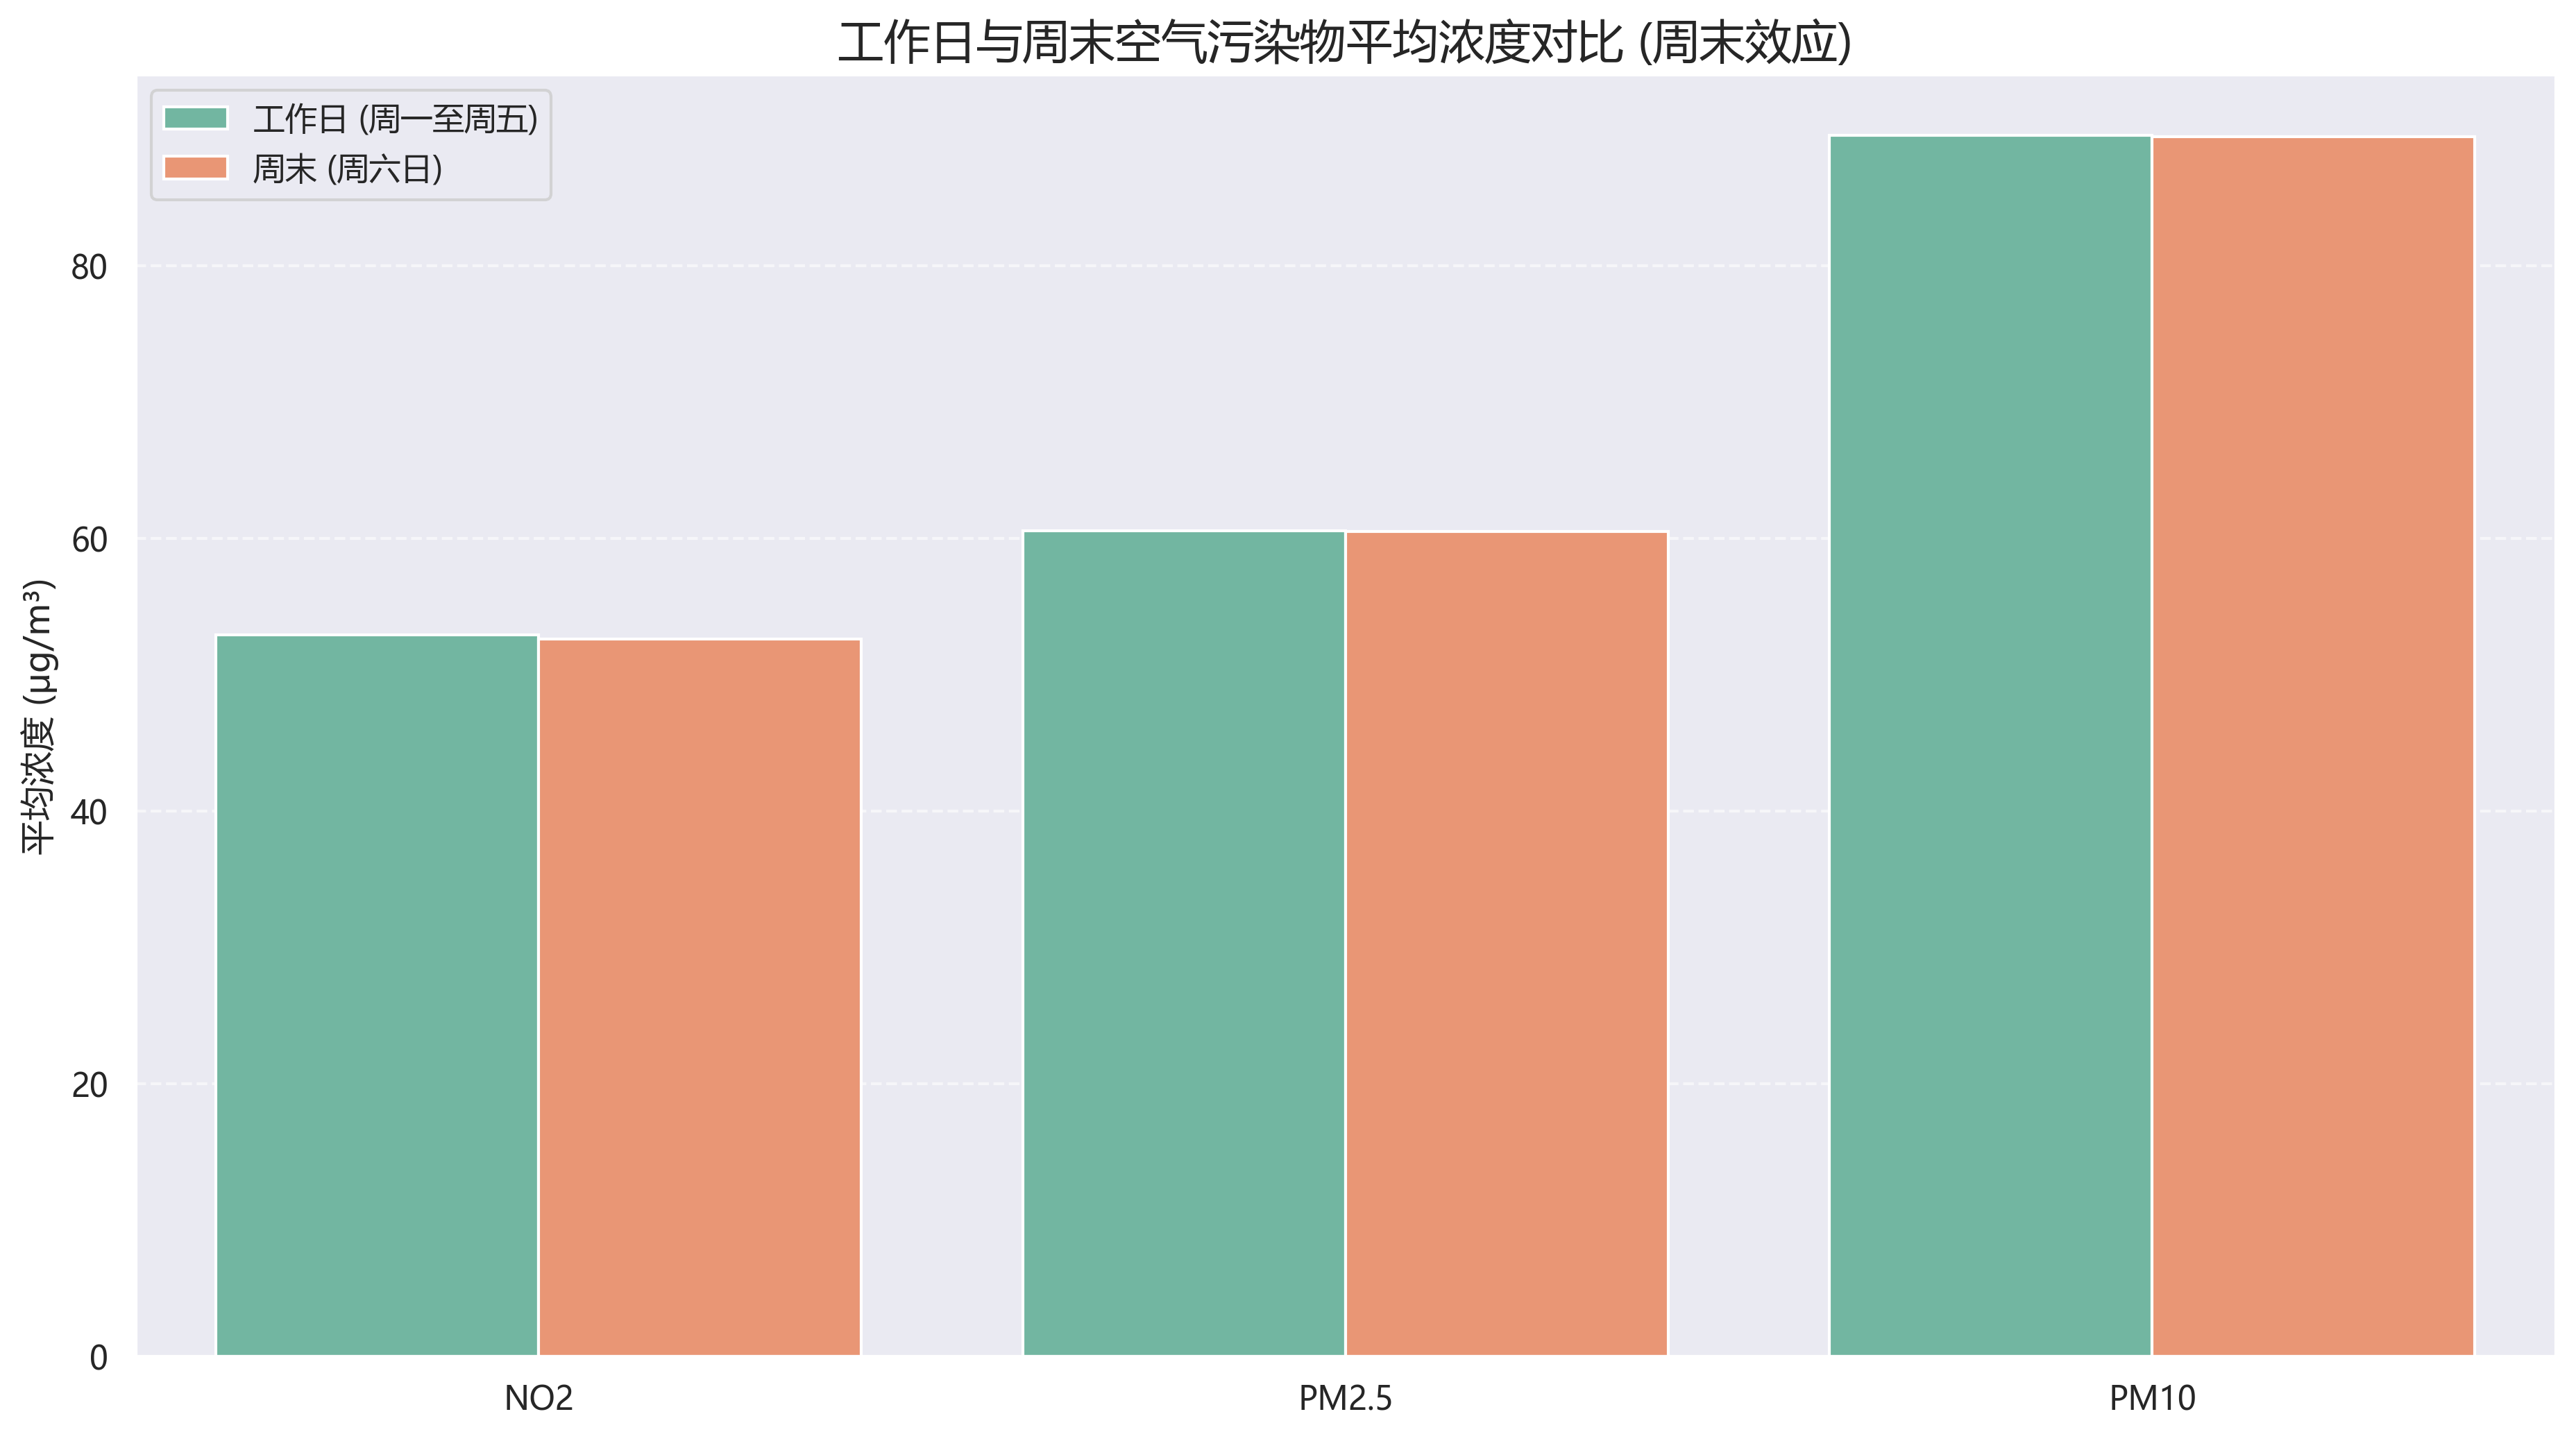
\includegraphics[width=0.7\textwidth]{images/3.png} 
    \caption{工作日与周末空气污染物平均浓度对比}
    \label{fig:24h_weekday_trend}
\end{figure}

我们推测：受地理位置因素影响，房山良乡是典型的大学城和城郊居住区，不像北京CBD或工业区有极强的“工作日通勤/生产”与“周末休息”的潮汐反差。这里的日常交通和生活排放相对平稳。
因此该区域为高教园区与居民区混合地带，日常人为活动及交通排放的周内波动较小，背景污染占主导地位。”

% \begin{figure}[htbp]
%     \centering
%     % width=0.8\textwidth 表示图片宽度占页面正文宽度的 80%
%     % 大括号里填你的图片文件名，不需要写后缀也能识别，但写上更保险
%     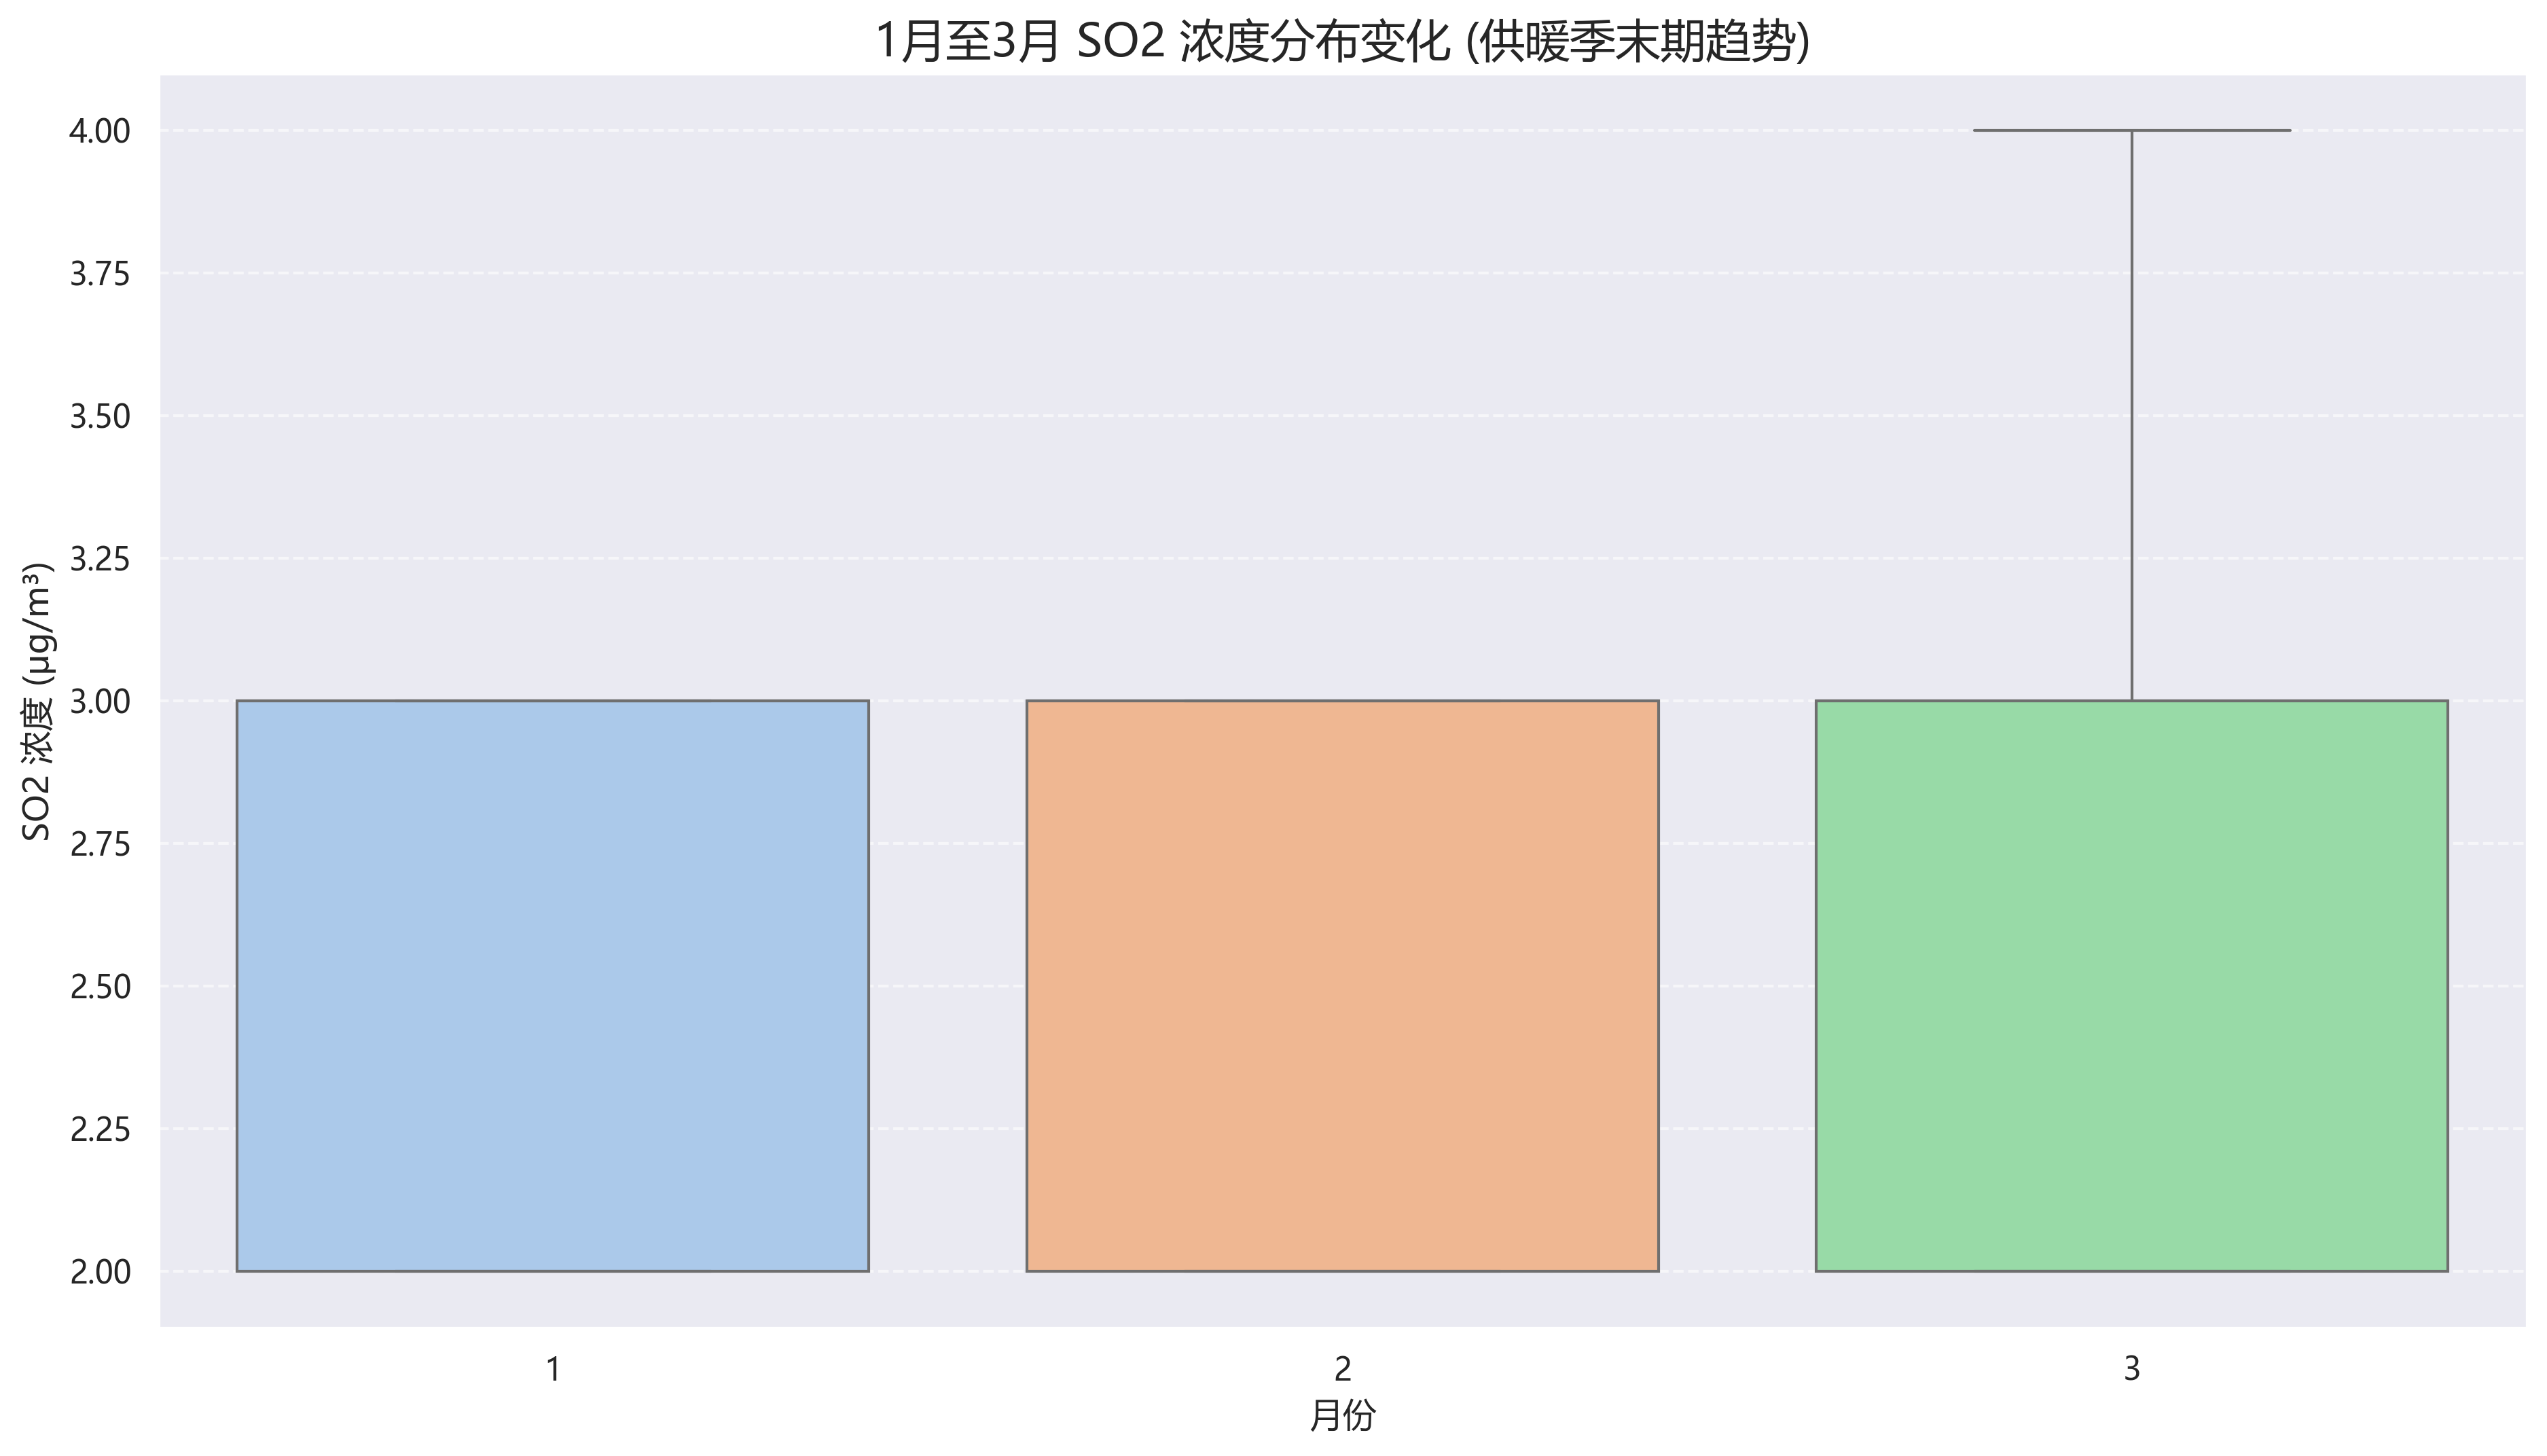
\includegraphics[width=1.1\textwidth]{images/4.png} 
    
%     \caption{良乡地区六种污染物 24 小时浓度日变化图} % 图片下方的标题
%     \label{fig:24h_trend} % 用于正文交叉引用的标签
% \end{figure}

\subsubsection{温度与湿度对污染物浓度的驱动机制分析}
在探究空气质量演化的动态过程之前，我们首先需要明确各污染物浓度与核心气象因子（温度、湿度）之间的静态关联程度。

\textbf{（1）基于 Spearman 相关性热力图的空气污染机理分析}

我们选用斯皮尔曼秩相关系数 (Spearman's Rank Correlation)\cite{spearman1904}。由于空气质量监测数据（如 PM2.5、SO$_2$ 等）通常呈现偏态分布，且气象因子对污染物的影响往往是非线性的，传统的皮尔逊（Pearson）相关系数（要求数据符合正态分布且仅能捕捉线性关系）可能无法准确反映变量间的本质联系。

因此，本文采用斯皮尔曼秩相关系数。这是一种非参数统计方法，通过变量的秩次（等级）而非原始数值来计算相关性，能够更严谨地衡量变量间的单调关系。其计算公式如下：
$$\rho = 1 - \frac{6 \sum d_i^2}{n(n^2 - 1)}$$其中，$d_i$ 为两变量秩次之差，$n$ 为样本量。
\bigskip
\begin{figure}[htbp]
    \centering
    % width=0.8\textwidth 表示图片宽度占页面正文宽度的 80%
    % 大括号里填你的图片文件名，不需要写后缀也能识别，但写上更保险
    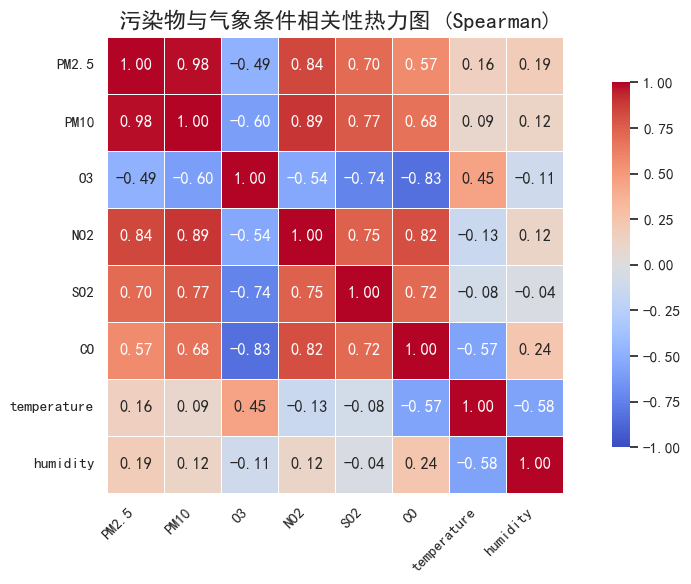
\includegraphics[width=0.8\textwidth]{images/5.png} 
    
    \caption{污染物与气象条件相关热力图} % 图片下方的标题
    \label{fig:hot} % 用于正文交叉引用的标签
\end{figure}


观察相关系数图中的 Spearman 相关系数矩阵，可以揭示良乡地区空气污染物的协同与拮抗机制，具体分析如下：
\bigskip
\begin{itemize}
    \item \textbf{气态污染物与颗粒物的“同源与同步富集”效应} \\
    热力图显示，左上角呈现明显的深红色高相关区。$PM_{2.5}$、$PM_{10}$、$NO_2$、$SO_2$ 和 $CO$ 之间均呈现极强的正相关性（相关系数 $\rho > 0.7$），其中 $PM_{2.5}$ 与 $PM_{10}$ 相关性高达 $0.98$，$PM_{2.5}$ 与 $NO_2$ 高达 $0.84$。
    
    \textbf{成因解释：} 这表明上述污染物在良乡地区具有高度的同源性。1月至3月处于采暖季，化石燃料燃烧与机动车尾气排放节奏高度一致。此外，这些污染物受相同的气象扩散条件制约，在夜间逆温或静稳天气下同步积累，在大风天气下同步稀释，呈现出“同步富集”特征。

    \item \textbf{$O_3$（臭氧）的独特“拮抗”现象与温度驱动} \\
    数据揭示 $O_3$ 展现出与所有其他污染物截然相反的特性，与 $NO_2$ ($\rho = -0.54$)、$CO$ ($\rho = -0.83$) 等呈\textbf{显著负相关}。同时，温度是唯一与 $O_3$ 呈显著正相关（$0.45$）的气象因素。
    
    \textbf{成因解释：} 这种全局负相关是典型的“大气光化学滴定效应”的体现。$O_3$ 的生成需要消耗 $NO_2$ 等前体物，且夜间高浓度的 $NO$ 会通过滴定反应大量消耗 $O_3$。因此，当一次污染物浓度处于高位时（常对应夜间或静稳天气），$O_3$ 恰好处于低值。而温度的升高通常伴随着太阳辐射的增强，加速了光化学反应速率，从而催化 $O_3$ 的生成。
\end{itemize}

\textbf{（2）温度对污染物浓度的多重影响}

为进一步揭示污染物浓度与气象因子间的非线性响应机制，本文选取相关性热力图中系数绝对值最大的两组特征对进行散点映射，并采用二阶多项式（Quadratic Fitting）进行曲线拟合
温度对空气质量的影响具有双重性。

\begin{figure}[htbp]
    \centering
    % 左侧子图
    \begin{subfigure}[b]{0.48\textwidth}
        \centering
        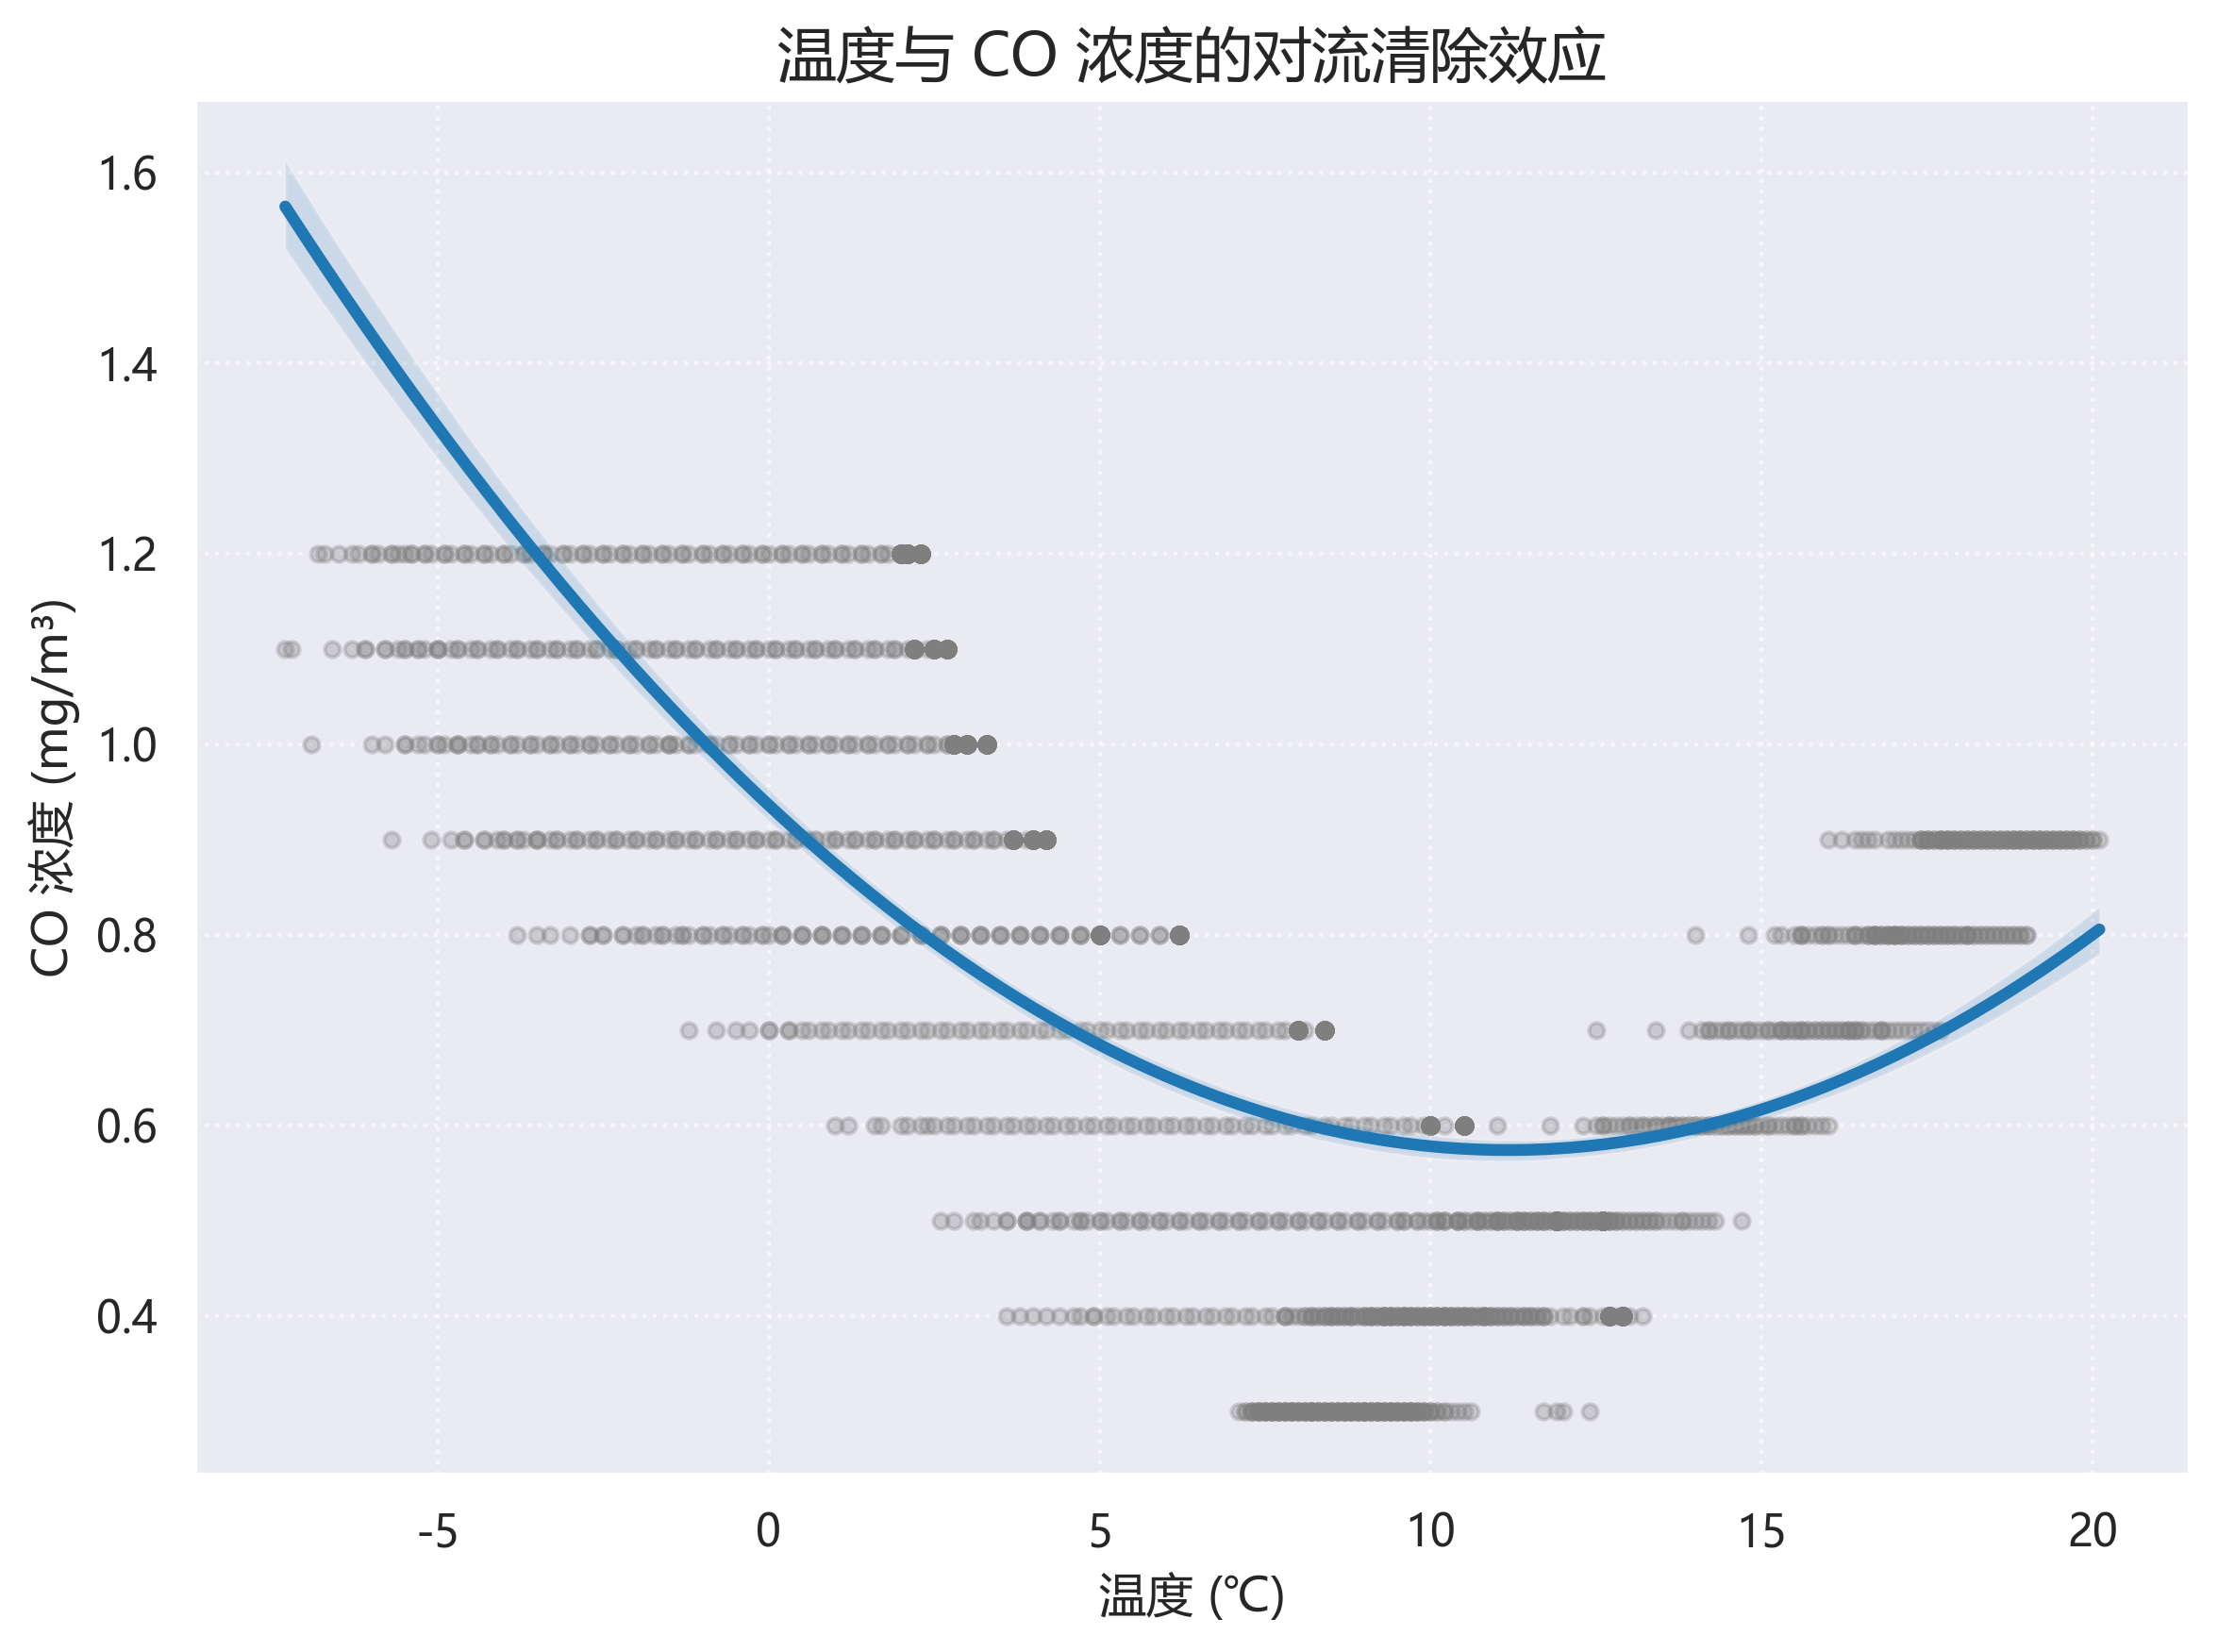
\includegraphics[width=\textwidth]{images/6.png} % 填入你的图片路径
        % \clip 后接参数可以切割图片，如果是一张图里的两个区域，建议先手动切成两张图
        \caption{温度与 $O_3$ 浓度的非线性响应关系}
        \label{fig:temp_o3}
    \end{subfigure}
    \hfill % 在两个子图之间插入弹性间距
    % 右侧子图
    \begin{subfigure}[b]{0.48\textwidth}
        \centering
        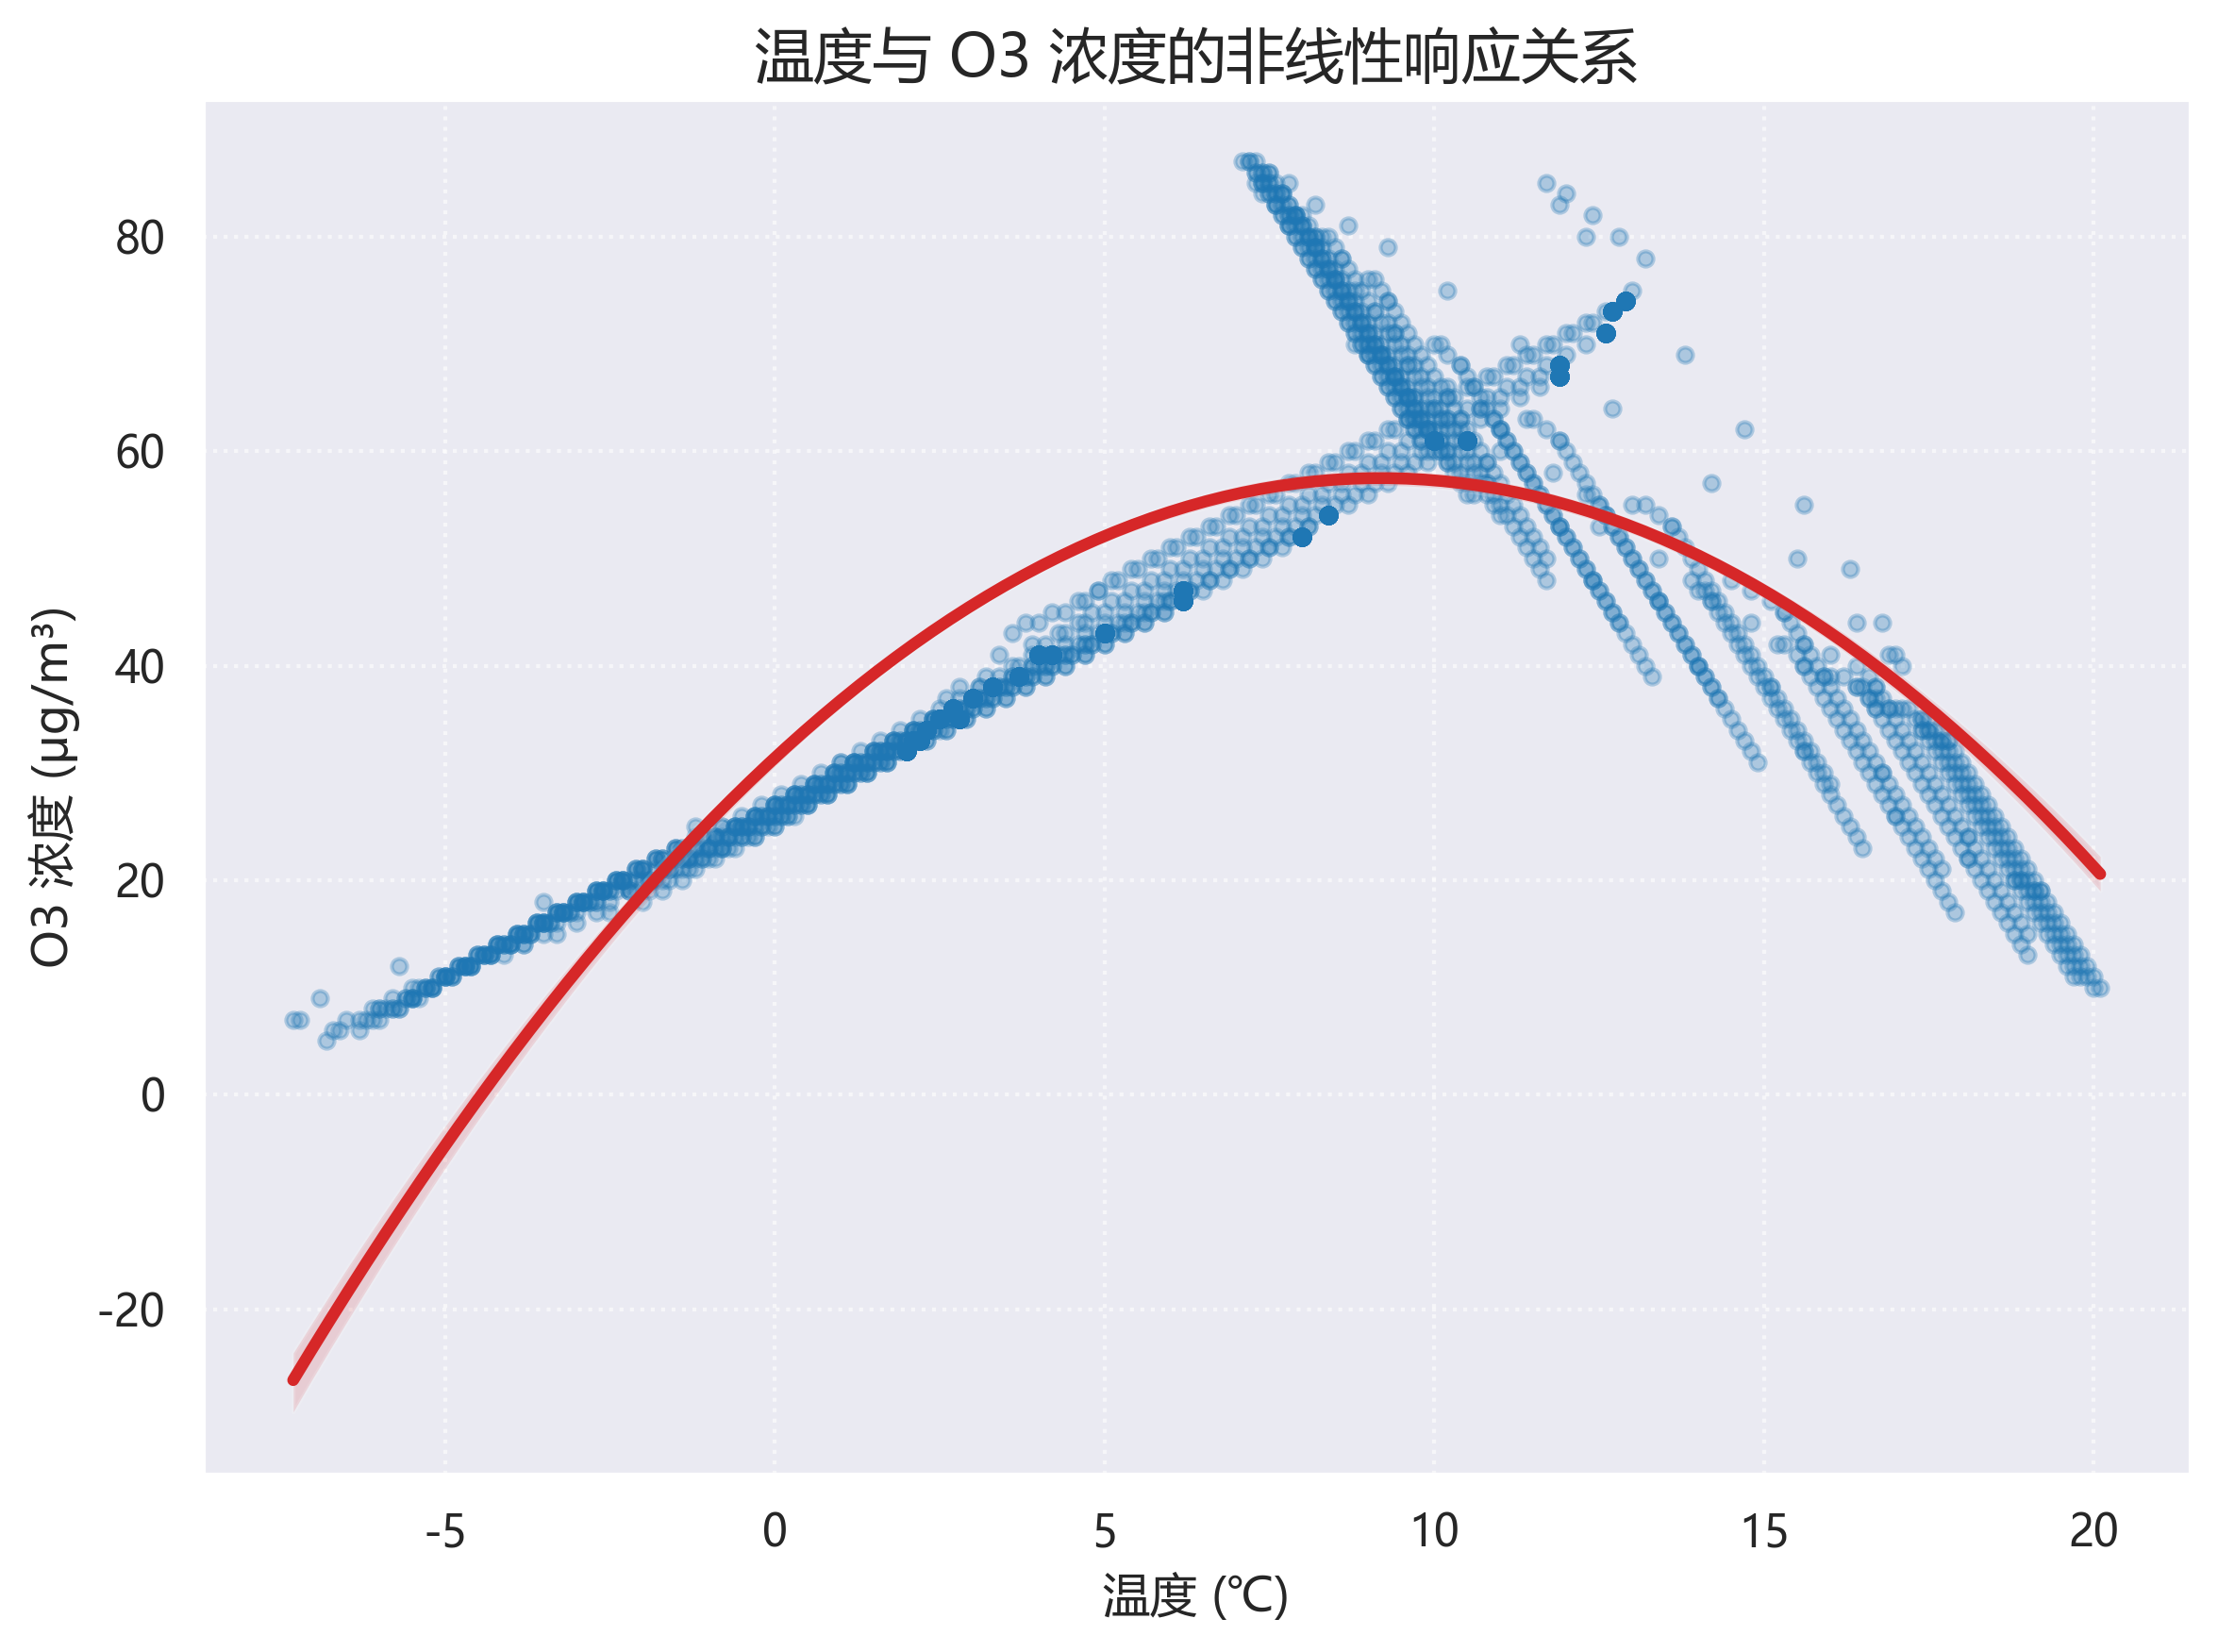
\includegraphics[width=\textwidth]{images/7.png}
        \caption{温度与 $CO$ 浓度的对流清除效应}
        \label{fig:temp_co}
    \end{subfigure}
    
    \caption{污染物浓度与温度的非线性拟合关系分析} % 整个大图的标题
    \label{fig:main_correlation}
\end{figure}
 
如图(a)所示，$O_3$ 浓度与温度呈现显著的非线性响应，拟合曲线呈倒“U”型趋势。
\begin{itemize}
    \item \textbf{上升段分析：} 在 $10^\circ C$ 以下区间，随着温度升高，$O_3$ 浓度迅速增加。这验证了高温通常伴随强紫外辐射，会加速前体物（$NO_x$ 与 VOCs）发生光化学反应生成臭氧的速率。
    \item \textbf{阈值制约：} 当温度接近 $20^\circ C$ 时，拟合曲线斜率出现平缓甚至下行。推测在特定前体物配比下，极高温可能改变了化学平衡或伴随扩散条件的改变（如对流增强），限制了臭氧的进一步富集。
\end{itemize}

如图(b) 所示，$CO$ 浓度随温度升高呈现出显著的“非线性衰减”特征。
\begin{itemize}
    \item \textbf{低温累积机制：} 当气温低于 $0^\circ C$ 时，$CO$ 浓度处于极高水平。这是由于北京 1--3 月处于采暖季，低温不仅导致源头排放增加，且易诱发逆温现象，将污染物压缩在近地面难以扩散。
    \item \textbf{热力清除效应：} 随着温度回升，地表受热引起垂直对流运动加强，大气边界层显著抬升。这种“热力对流”如同排风扇将积聚在近地面的一次污染物迅速向上稀释，形成明显的对流清除效应。
\end{itemize}



\subsubsection{温湿度影响的滞后效应分析}
空气质量的变化并非仅取决于当前时刻的气象状态，往往受到过去一段时间气象条件的持续驱动与累积影响。例如，环境温度的升高通常需要一定的时间传导以激发光化学反应产生臭氧，而湿度的持续累积对气溶胶吸湿增长也存在物理尺度上的延迟效应。

为了定量评估气象因子对污染物影响的滞后程度，本文引入时滞相关分析（Time-lagged Correlation Analysis）。定义当前 $t$ 时刻的某污染物浓度为 $C_t$，计算其与滞后阶数为 $L$（$L = 0, 1, \dots, 6$ 小时）的气象因子 $W_{t-L}$ 之间的斯皮尔曼秩相关系数 $\rho_L$：

\begin{equation}
\rho_L = \text{Corr}(C_t, W_{t-L})
\end{equation}

其中，$L$ 代表气象因子领先于污染物浓度的时长。利用特征工程中构造的 \texttt{temperature\_lag} 和 \texttt{humidity\_lag} 系列特征，本文对不同滞后阶数下的关联强度进行了测算。

通过观察滞后趋势图，可以得出以下分析结论：
\begin{itemize}
    \item \textbf{气象因子驱动的极性差异} \\
    温度与 $O_3$ 呈现显著的正相关滞后响应，而与 $CO$ 呈现显著的负相关滞后响应，且相关系数绝对值在所有污染物中最高。这表明温度是良乡地区空气质量演化的核心动力因子。
    \item \textbf{污染物的滞后响应特征}
    \begin{enumerate}
        \item \textbf{长效累积型：} 观察发现，$PM_{2.5}$、$PM_{10}$ 以及 $SO_2$ 与温度的相关性随着滞后时间的增加（从 Lag 0 到 Lag 3）呈现上升趋势。这说明颗粒物受温度的影响具有明显的累积效应，过去 $2 \sim 3$ 小时的气象条件对当前浓度的解释力更强。
        \item \textbf{衰减响应型：} 相对湿度对 $PM_{2.5}$ 和 $CO$ 的影响在滞后 1 小时后开始逐渐减弱。$NO_2$ 对温度和湿度的响应均随滞后阶数增加而减弱，说明其受实时气象驱动更为直接。
    \end{enumerate}

\end{itemize}

\begin{figure}[h]
    \centering
    % width=0.8\textwidth 表示图片宽度占页面正文宽度的 80%
    % 大括号里填你的图片文件名，不需要写后缀也能识别，但写上更保险
    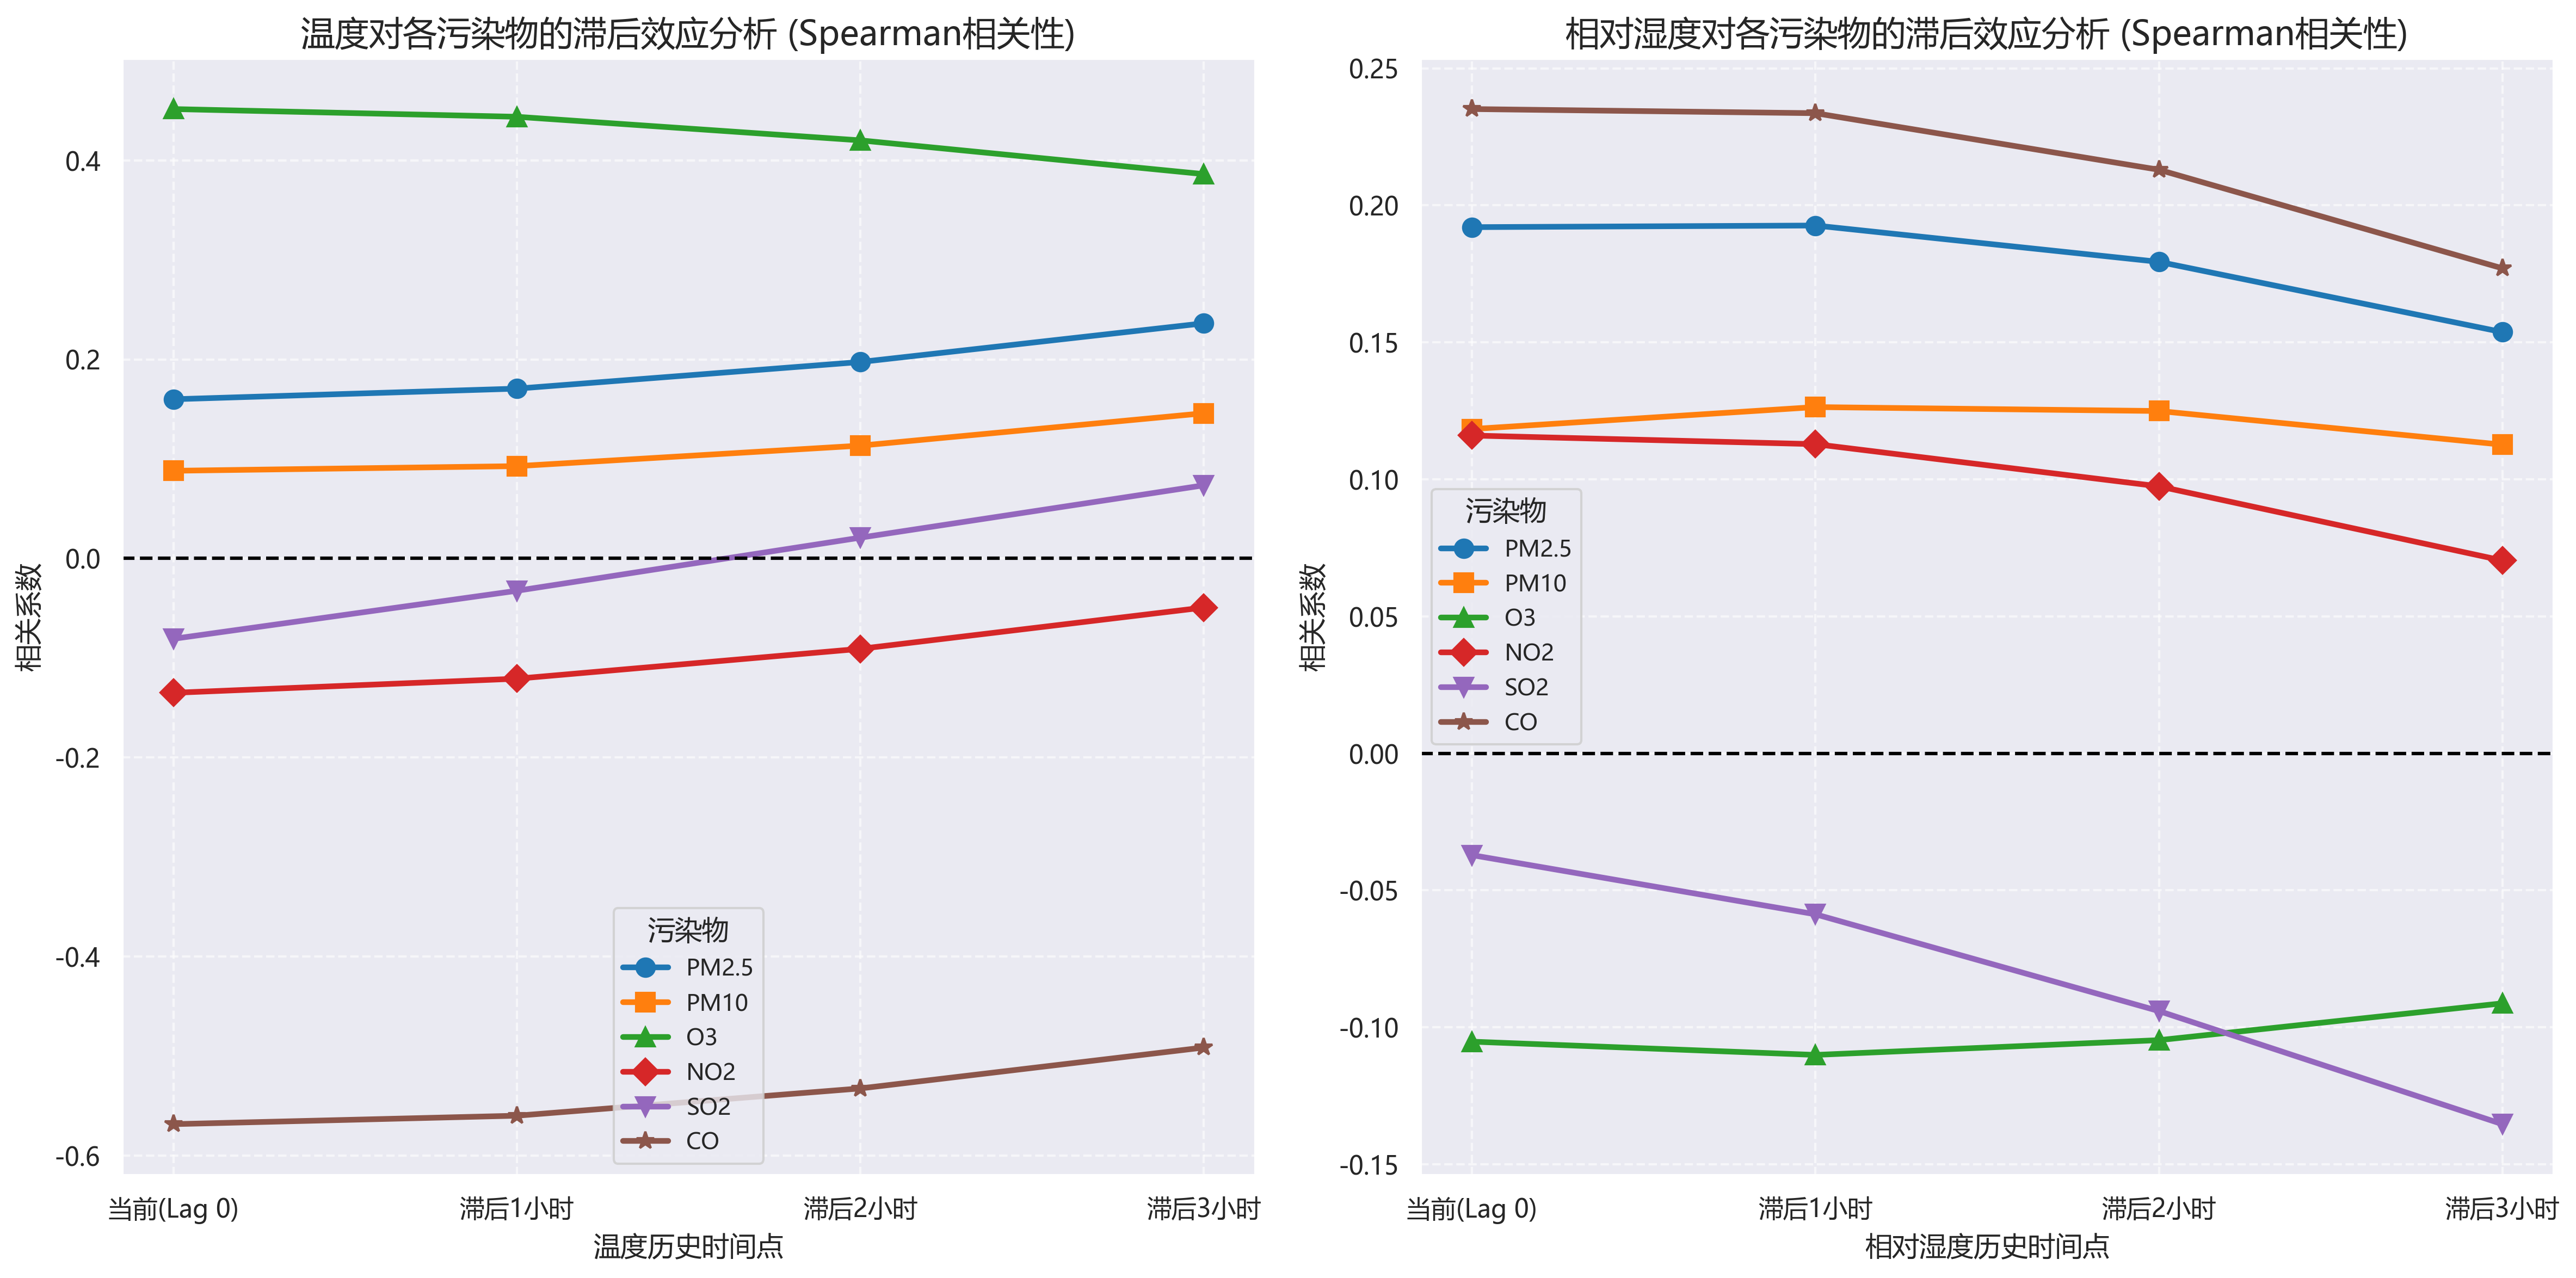
\includegraphics[width=1.0\textwidth]{images/8.png} 
    \caption{污染物与气象条件相关热力图} % 图片下方的标题
    \label{fig:hot2} % 用于正文交叉引用的标签
\end{figure}

\subsection{问题二：建立 BiLSTM + XGBoost 级联融合模型}

\subsubsection{联合建模逻辑}
针对问题二，我们基于前面分析的特征工程和污染物间的协同关系，同时为了捕捉六种污染物（$PM_{2.5}, PM_{10}, O_3, NO_2, SO_2, CO$）之间的协同变化规律，本文摒弃了传统的多个独立单目标模型，采用 \textbf{BiLSTM + XGBoost} 进行联合建模。该模型在每一次迭代建树时，共享输入层的气象与时间特征，能够隐式学习污染物之间（如前体物 $NO_2$ 与二次产物 $O_3$）的物理化学耦合关系。

% 为实现两类算法的优势互补，本文引入集成学习中的 Stacking 思想，设计了如下两层训练体系（如图 \ref{fig:stacking_arch} 所示）：

\begin{figure}[htbp]
    \centering
    % width=0.8\textwidth 表示图片宽度占页面正文宽度的 80%
    % 大括号里填你的图片文件名，不需要写后缀也能识别，但写上更保险
    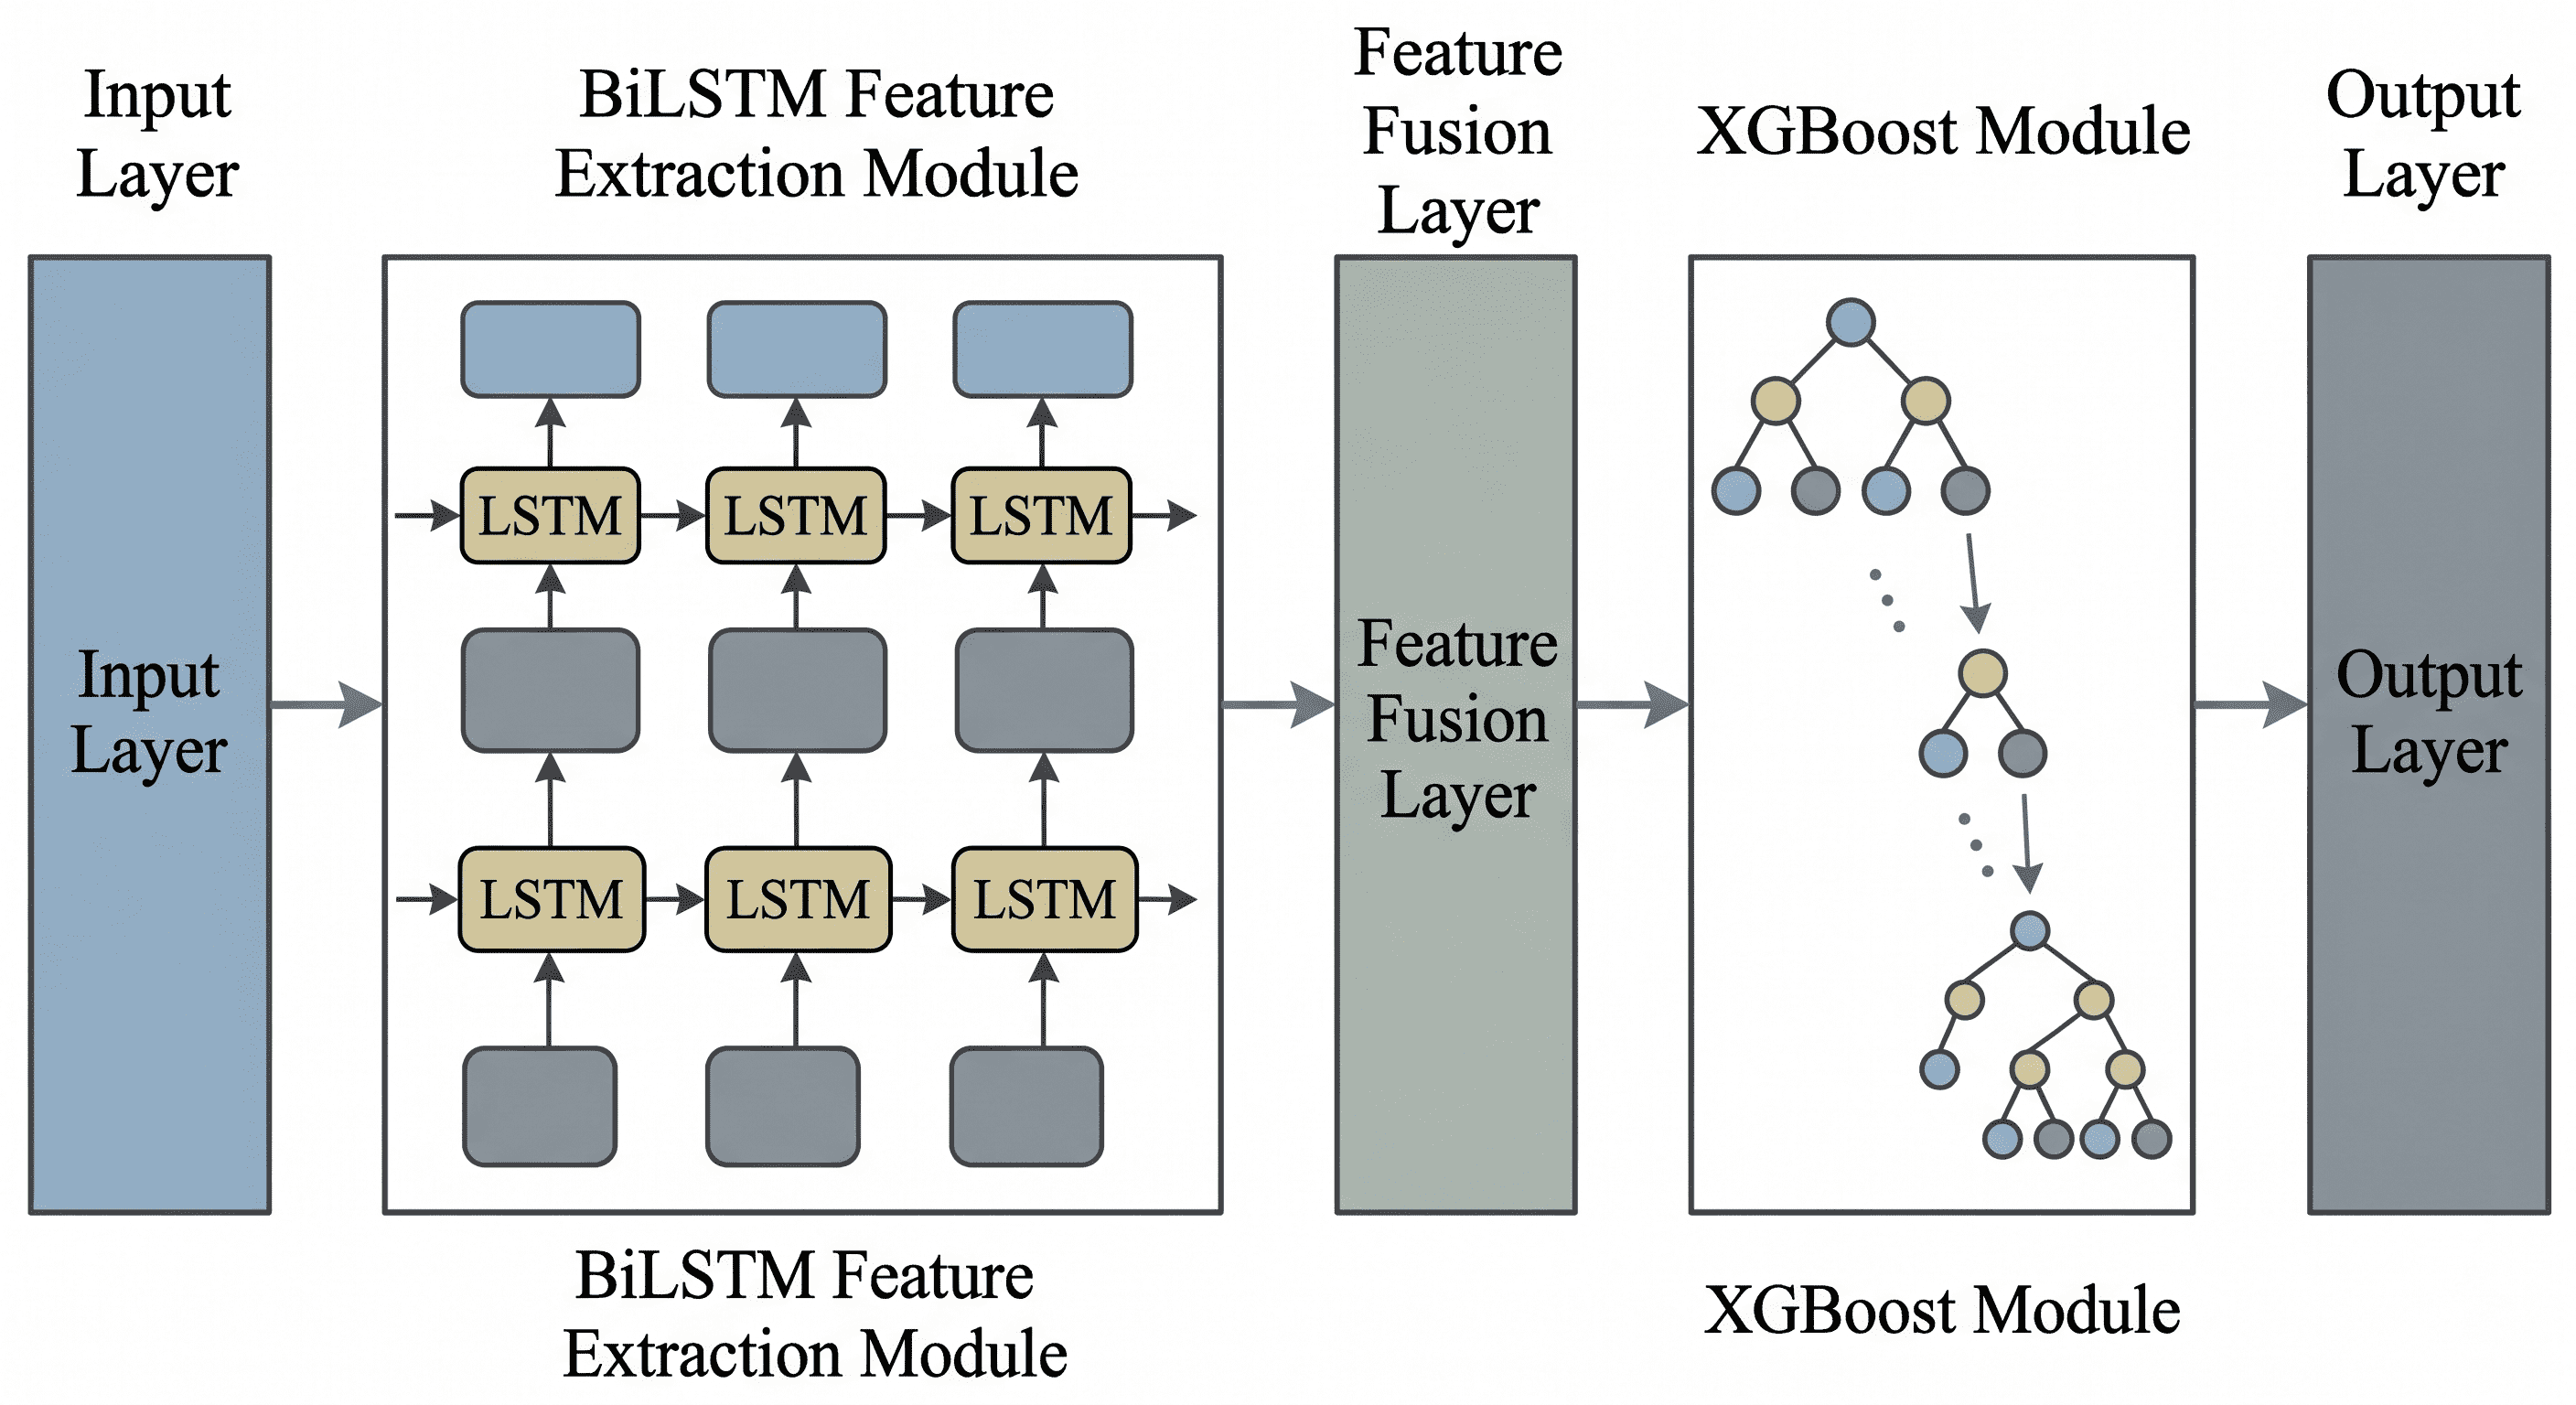
\includegraphics[width=0.9\textwidth]{images/model.png} 
    \caption{BiLSTM + XGBoost 级联融合模型示意图} % 图片下方的标题
    \label{fig:model} % 用于正文交叉引用的标签
\end{figure}


\begin{itemize}
    \item \textbf{第一层：基模型——深度时序特征提取} \\
    本文首先利用 \textbf{BiLSTM} 网络作为基学习器。通过双向门控机制\cite{bilstm}，令过去 3 小时的温湿度与污染物浓度序列正向和反向流过网络。BiLSTM 能够从动态变化的观测序列中挖掘出深层时序隐藏特征 $\mathbf{H}_{\text{hidden}}$，并输出第一阶段的协同预测结果 $\hat{\mathbf{Y}}_{\text{initial}}$。

    \item \textbf{第二层：元模型——残差修正与非线性融合} \\
    本文将第一层 BiLSTM 输出的预测结果作为先验知识，与原始的气象衍生特征、正余弦时间特征进行特征拼接（Feature Concatenation）。该组合特征被输入到 \textbf{Multi-Output XGBoost} 结构中进行二次训练\cite{xgboost}。在此框架下，XGBoost 扮演“误差修正器”与“全局特征融合器”的角色，利用其强大的非线性拟合能力修正 BiLSTM 的预测残差，从而大幅提升模型的鲁棒性与预测精度。
\end{itemize}


为实现两类算法的优势互补，本文引入集成学习中的 Stacking 思想
\begin{equation}
 \mathbf{\hat{Y}}_{\text{final}} = \mathcal{F}_{\text{XGB}} \left( \mathcal{F}_{\text{BiLSTM}}(X_{\text{seq}}) \oplus X_{\text{static}} \right)
\end{equation}

其中各参数含义为：
\begin{itemize}[itemsep=0pt, parsep=0pt, topsep=0pt]
\item $\mathbf{\hat{Y}}_{\text{final}}$：模型最终输出的 $t+1$ 时刻六种污染物浓度的预测向量。
\item $\mathcal{F}_{\text{BiLSTM}}(X_{\text{seq}})$：基学习器（第一层）。处理过去 3 小时的历史序列 $X_{\text{seq}}$，输出深层时序隐藏特征作为先验知识。
\item $X_{\text{static}}$：原始截面特征，包括温湿度衍生特征、正余弦时间编码及供暖期标签等。
\item $\oplus$：特征拼接算子（Feature Concatenation），将时序特征与静态特征向量化合并。
\item $\mathcal{F}_{\text{XGB}}$：元学习器（第二层）。利用 Multi-Output XGBoost 对组合特征进行二次训练，修正残差并实现协同预测。
\end{itemize}

% 对于包含 $m$ 个输出变量（本文中 $m=6$）的协同预测任务，第 $t$ 轮迭代的目标函数 $Obj^{(t)}$ 定义为多维输出联合残差的极小化：

% \begin{equation}
% Obj^{(t)} = \sum_{j=1}^{m} \left[ \sum_{i=1}^{n} L(y_{i,j}, \hat{y}_{i,j}^{(t-1)} + f_t(x_i)) \right] + \Omega(f_t)
% \end{equation}

% 其中：
% \begin{itemize}
%     \item $n$ 为样本数量，$m=6$ 为协同预测的污染物维度。
%     \item $y_{i,j}$ 为第 $i$ 个样本中第 $j$ 种污染物的真实浓度值。
%     \item $\hat{y}_{i,j}^{(t-1)}$ 为上一轮迭代后的预测值。
%     \item $f_t(x_i)$ 为本轮迭代中所有输出变量共享的弱学习器（决策树）。
%     \item $\Omega(f_t)$ 为正则化项，用于惩罚模型复杂度以防止过拟合。
% \end{itemize}

模型通过对输入空间 $\mathcal{X}$（含时间周期、温湿度滞后特征及气象衍生特征）到多维污染物空间 $\mathcal{Y}$ 的映射，实现联合预测：

\begin{equation}
\begin{bmatrix} 
\hat{PM}_{2.5} \\ \hat{PM}_{10} \\ \hat{O}_3 \\ \hat{NO}_2 \\ \hat{SO}_2 \\ \hat{CO} 
\end{bmatrix}_{t+1} = \sum_{k=1}^{K} f_k \left( \mathbf{X}_{time}, \mathbf{X}_{weather}, \mathbf{X}_{lags} \right)
\end{equation}

通过这种协同学习机制，模型不仅能够拟合单一污染物的浓度数值，更能在预测过程中保持不同污染物之间协方差结构的一致性 $\text{Cov}(\hat{y}_j, \hat{y}_k) \neq 0$，从而更准确地反映区域空气质量的整体演化规律。

\begin{table}[htbp]
    \centering
    \caption{BiLSTM-XGBoost 级联模型测试集评估结果}
    \label{tab:evaluation_results}
    % 使用 tabularx 确保表格宽度自适应，Y 格式平分宽度并居中
    \begin{tabularx}{\textwidth}{@{} YYYY @{}} 
        \toprule
        \textbf{污染物} & \textbf{RMSE} & \textbf{MAE} & \textbf{$R^2$} \\
        \midrule
        $PM_{2.5}$ & 5.5239 & 3.8721 & 0.8439 \\
        $PM_{10}$  & 9.4016 & 6.8562 & 0.8452 \\
        $O_3$      & 3.6329 & 2.6966 & 0.9663 \\
        $NO_2$     & 2.1756 & 1.6005 & 0.9753 \\
        $SO_2$     & 0.0707 & 0.0359 & 0.9925 \\
        $CO$       & 0.0226 & 0.0146 & 0.9897 \\
        \bottomrule
    \end{tabularx}
\end{table}

模型在测试集上表现出卓越的拟合性能，其中 SO2、CO 等污染物的决定系数 ($R^2$) 高达 0.97 以上，PM10 与 PM2.5 亦保持在 0.8 左右的高位。

\subsubsection{多目标预测追踪分析与可靠性验证}

为了直观验证BiLSTM + XGBoost 级联融合模型在多污染物协同预测任务中的可靠性，本文从测试集中截取了连续 120 小时（2026年3月16日至3月21日）的预测结果，并与实际观测值（Ground Truth）进行对比追踪，如图~\ref{fig:prediction_tracking} 所示。

\begin{figure}[htbp]
    \centering
    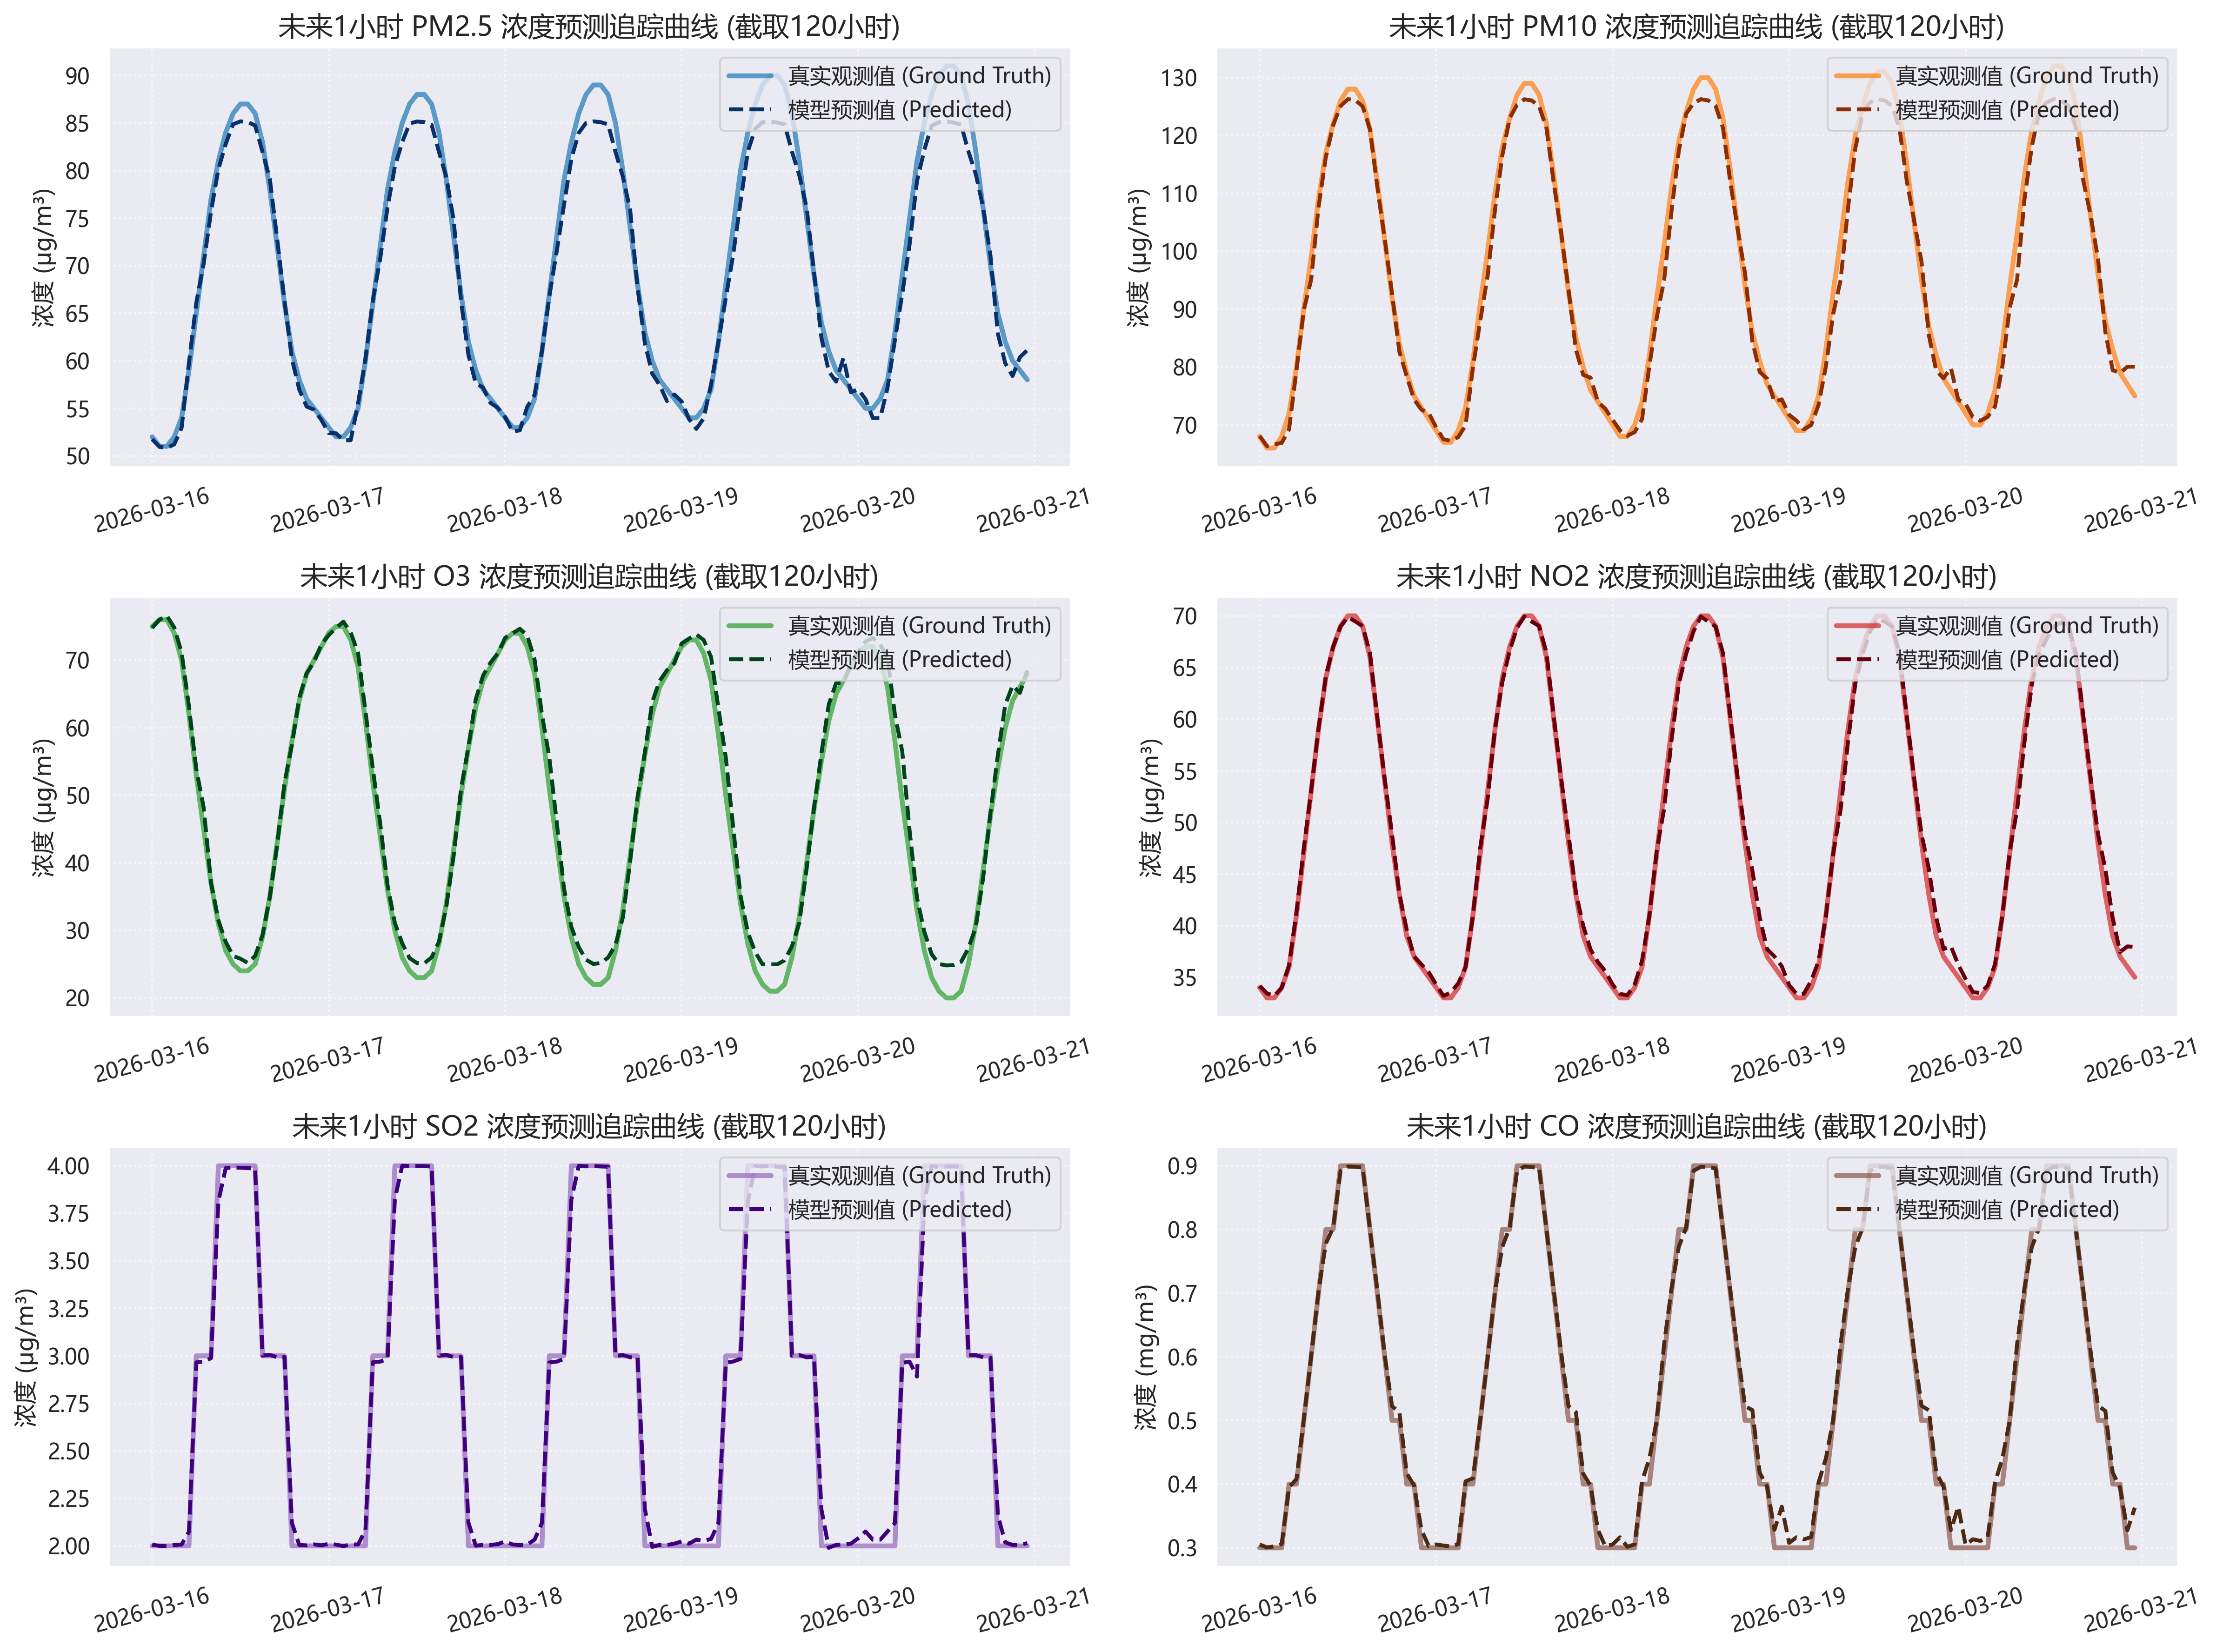
\includegraphics[width=0.9\textwidth]{images/9.png} % 替换为你的图片路径
    \caption{六种主要污染物未来 1 小时浓度预测追踪曲线对比图}
    \label{fig:prediction_tracking}
\end{figure}

基于 BiLSTM + XGBoost 级联融合模型构建的多变量协同预测模型在测试集上展现出了卓越的拟合性能（如图~\ref{fig:prediction_tracking} 所示）。截取连续 120 小时的预测时序追踪曲线可知：
\begin{itemize}
    \item \textbf{高拟合精度：} 模型预测值（虚线）与真实观测值（实线）在整体趋势上保持高度重合，能够准确捕捉到各污染物在早晚高峰时段的浓度峰值以及午后的低谷波动。
    \item \textbf{协同演化同步性：} 结果显示模型成功捕捉了 $PM_{2.5}$ 与 $PM_{10}$、以及 $NO_2$ 与 $CO$ 之间近乎同步的波动特征，证明了联合建模在处理同源排放污染物时的优越性。
    \item \textbf{极端波动捕捉：} 即使在 $SO_2$ 和 $CO$ 出现阶梯式或剧烈变化的时刻，预测曲线仍能迅速跟进。这表明通过引入滞后特征与温湿度非线性特征，模型具备了较强的鲁棒性与实时修正能力。
\end{itemize}
综上表明，该模型不仅具备单变量的时序外推能力，更成功内化了由气象驱动的多变量联合演化规律。


\subsubsection{全局特征重要性规律机制提取}

对于协同预测模型中的每一个决策树 $f_k$，特征 $X_j$ 的重要性通过该特征在所有分裂节点上带来的增益（Gain）总和来衡量。在多输出框架下，由于模型共享了输入特征空间，我们可以构建出描述“输入特征 $\to$ 预测目标”驱动强度的全局重要性矩阵 $\mathbf{M}$：
\begin{equation}
    M_{i,j} = \frac{1}{N_{trees}} \sum_{t=1}^{N_{trees}} \text{Gain}(Feature_i, Target_j)
\end{equation}
其中，$M_{i,j}$ 代表第 $i$ 个输入特征对第 $j$ 种污染物预测的权重贡献。

为了进一步探究良乡地区空气质量演化的内在驱动机制，本文利用训练好的 Multi-Output XGBoost 模型提取了特征重要性矩阵。该矩阵揭示了各输入特征（气象、时间及历史浓度）对六种污染物 $t+1$ 时刻浓度预测的贡献程度，从而实现了对污染物“协同变化规律”的量化提取。

观察图~\ref{fig:importance_heatmap} 的特征驱动矩阵，可以提取出以下关键协同演化规律：
\begin{itemize}
    \item \textbf{污染物的强时序惯性与滞后驱动：} 矩阵对角线附近存在明显的权重聚集。例如，$SO_{2\_lag1}$ 对未来一小时 $SO_2$ 的驱动权重高达 $0.518$，对 $CO$ 的驱动权重甚至达到 $0.643$。这表明良乡地区的一次污染物具有极强的时序相关性，历史浓度是预测未来的核心基准。
    \item \textbf{$NO_2$ 的全局前体物效应：} 实验发现 $NO_2$ 是影响所有污染物预测的关键特征。它对 $PM_{2.5}$ ($0.375$)、$PM_{10}$ ($0.485$) 及自身 ($0.541$) 均展现出极高的解释力。这印证了 $NO_2$ 作为机动车尾气的主要成分，不仅直接决定了氮氧化物水平，还通过光化学反应促进了二次颗粒物的生成。
    \item \textbf{气象因子的长效制约：} 滞后 3 小时的特征（如 $NO_{2\_lag3}, PM_{10\_lag3}$）依然保持了一定的权重（$0.04 \sim 0.05$），证明了环境状态对空气质量的影响具有典型的累积效应和滞后特征。
\end{itemize}

\begin{figure}[htbp]
    \centering
    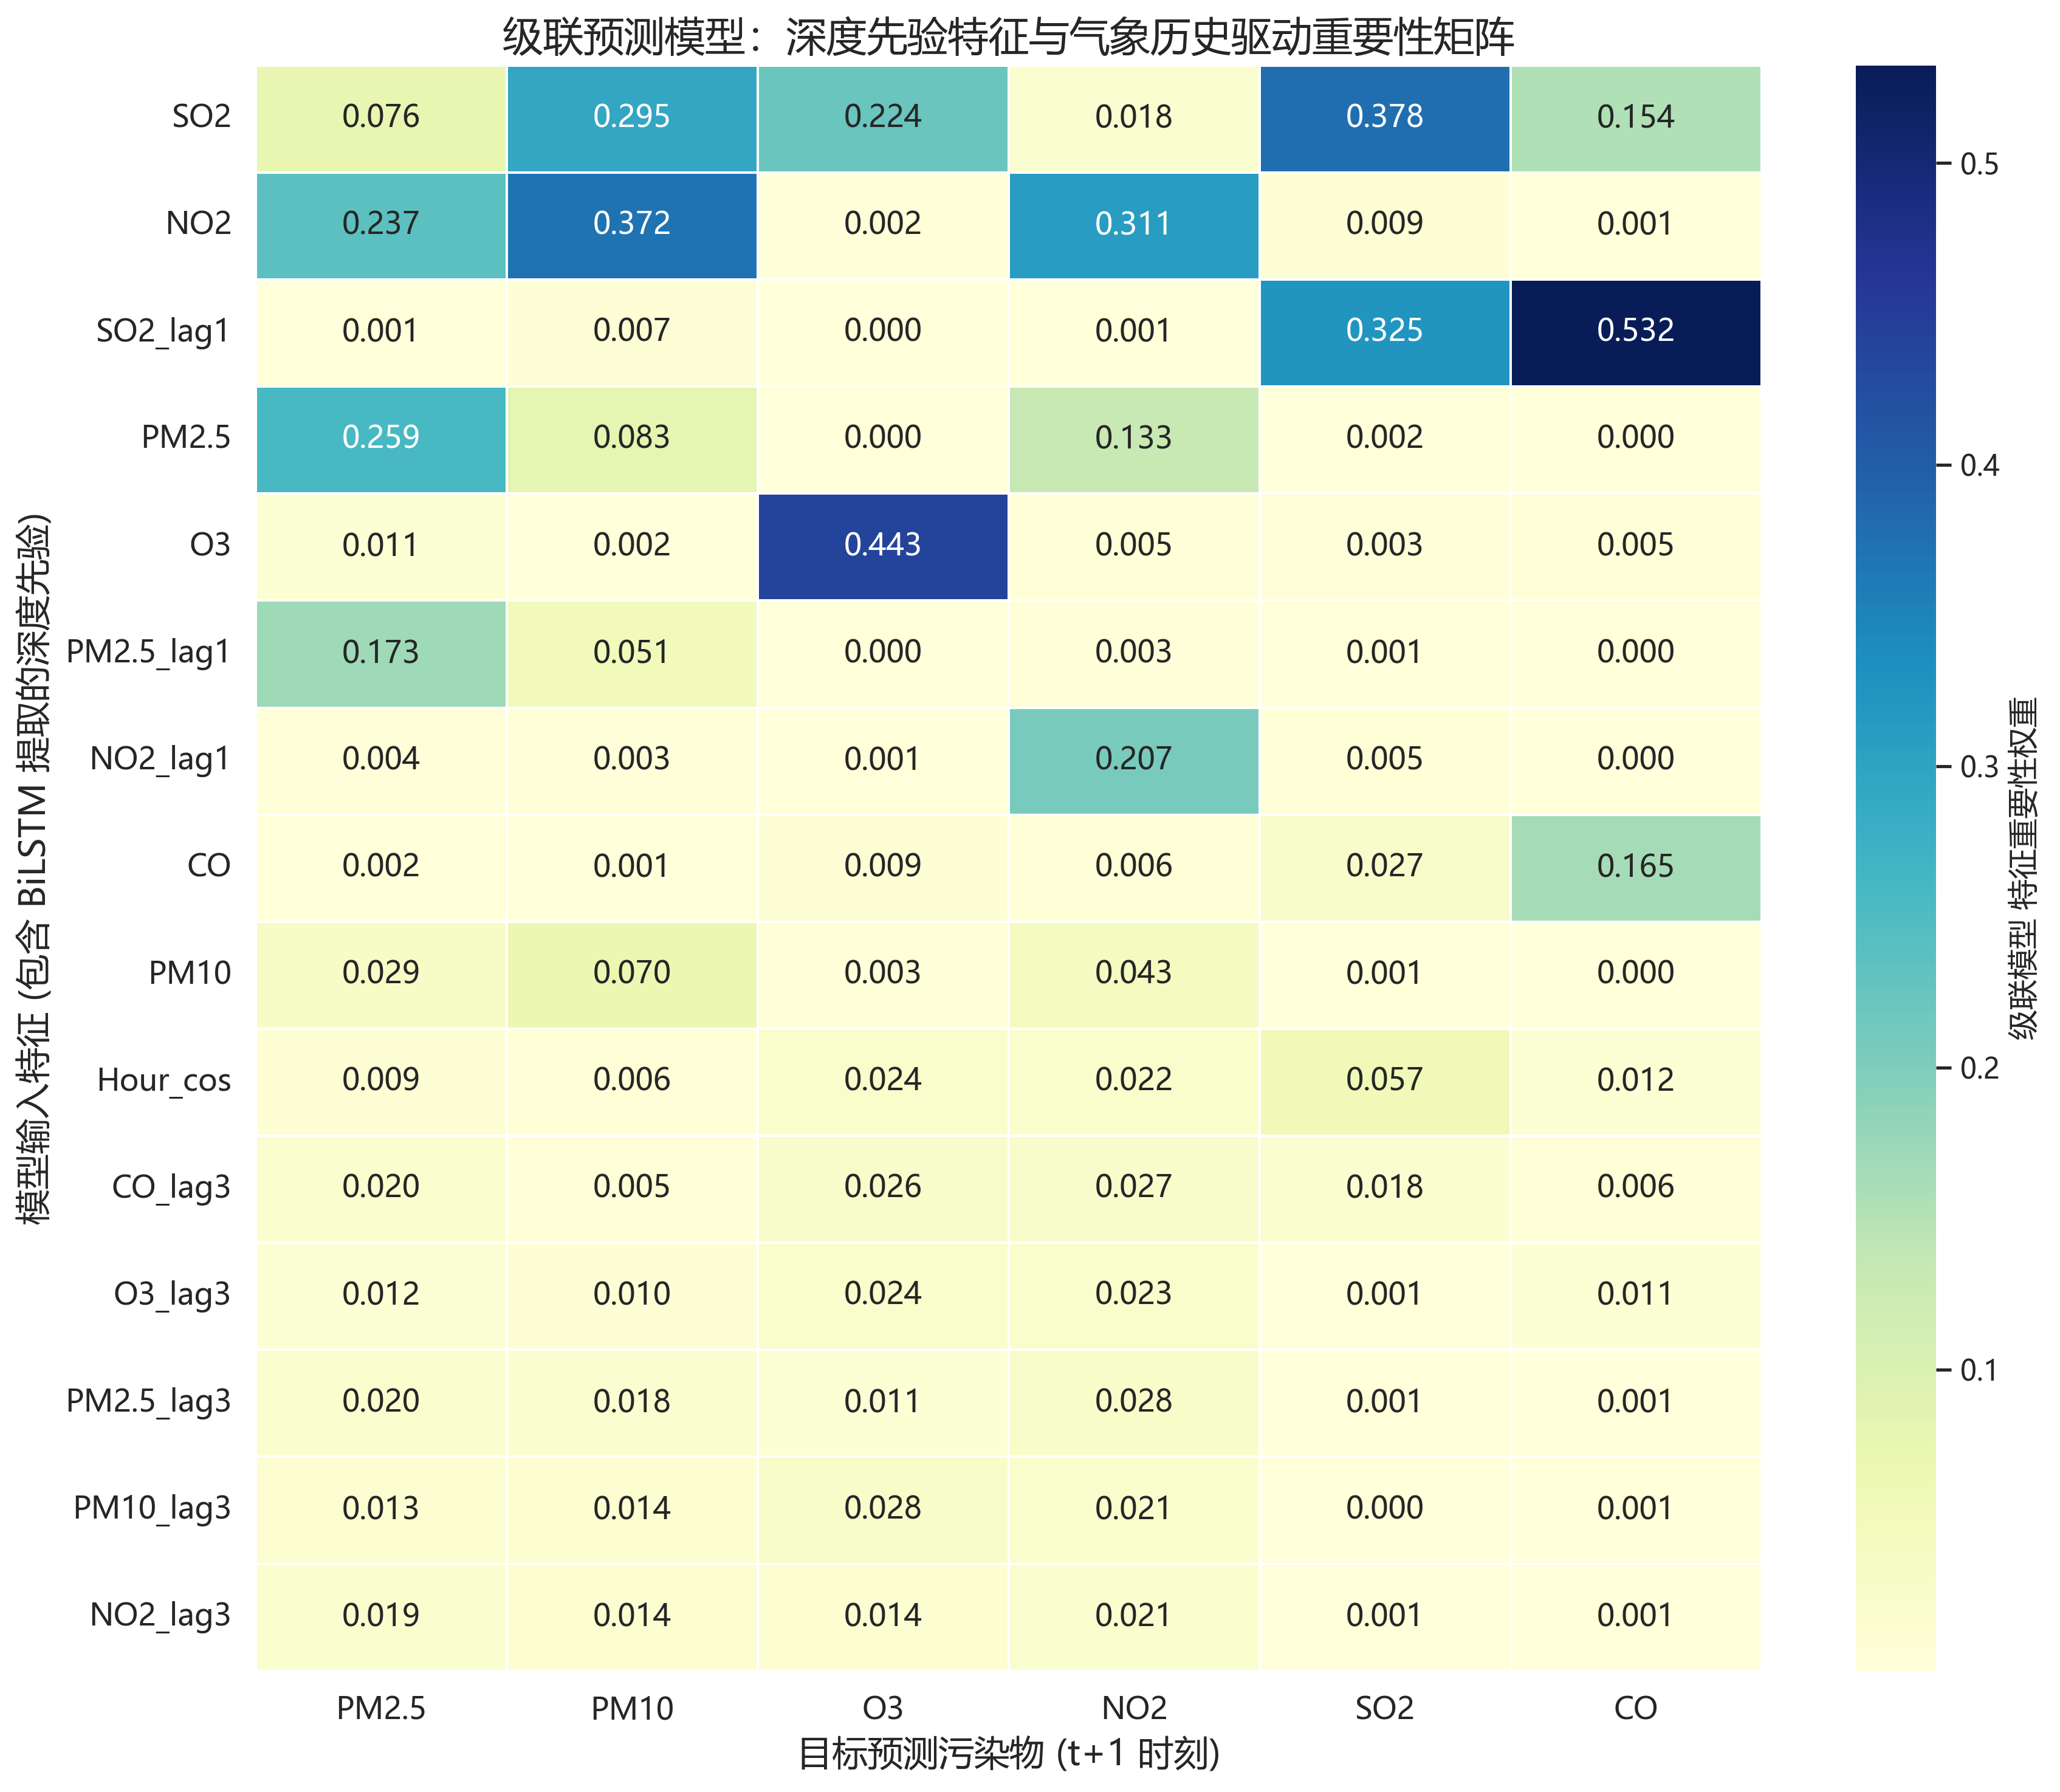
\includegraphics[width=0.62\textwidth]{images/10.png} % 替换为你的图片路径
    \caption{特征重要性热力图：输入特征对六种污染物预测的权重贡献矩阵} % 图片下方的标题
    \label{fig:importance_heatmap}
\end{figure}
\newpage
\subsubsection{基于 SHAP 归因理论的污染物协同变化机制解锁}

传统的集成树模型特征重要性度量仅能反映变量的全局贡献权重，无法揭示特征与目标值间的方向性作用（正向促进或负向抑制）。为深度解析六种污染物的协同演化规律，本文引入基于博弈论的 \textbf{SHAP (SHapley Additive exPlanations)} 归因算法进行模型的可解释性分析。通过对典型颗粒物（$\text{PM}_{2.5}$）与光化学气体（$\text{O}_3$）的 SHAP 蜂群图进行定量挖掘（见图 \ref{fig:shap_pm25} 与图 \ref{fig:shap_o3}），模型自主提取出以下三大核心物理化学驱动机制：

\begin{figure}[htbp]
    \centering
    % 左侧子图
    \begin{subfigure}[b]{0.48\textwidth}
        \centering
        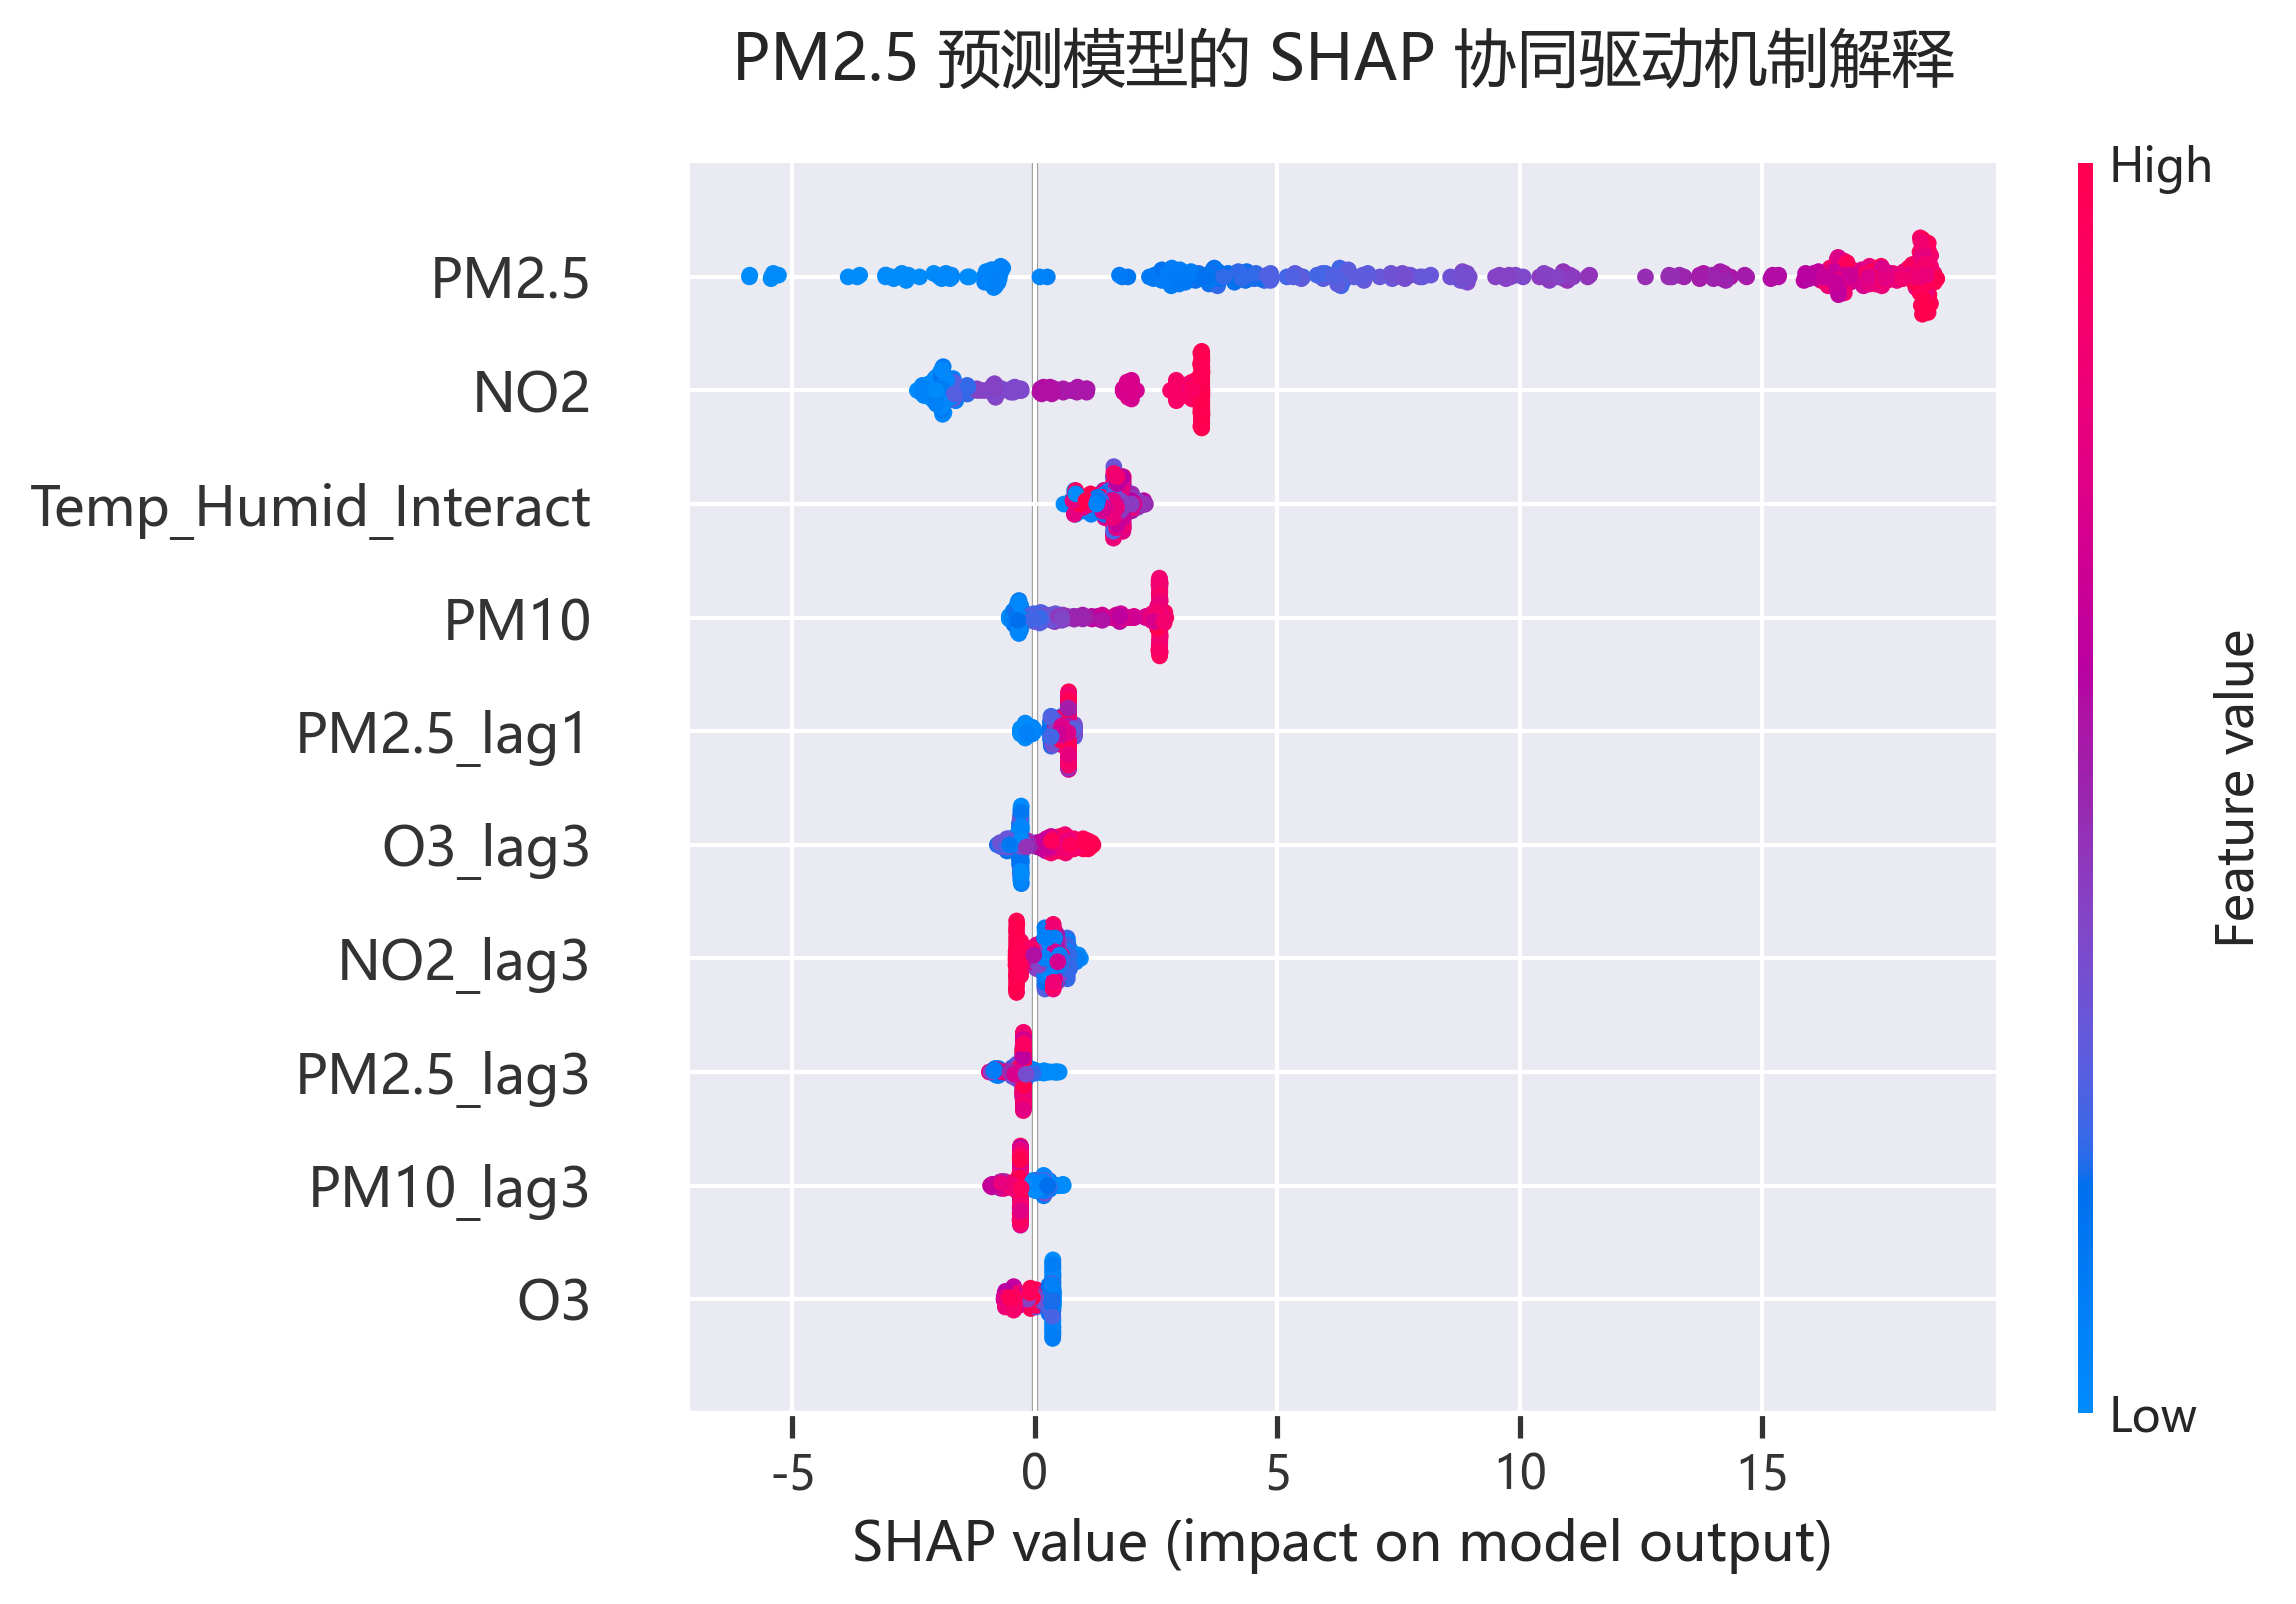
\includegraphics[width=\textwidth]{images/shap_pm25.png}
        \caption{$\text{PM}_{2.5}$ 协同驱动机制 SHAP 图}
        \label{fig:shap_pm25}
    \end{subfigure}
    \hfill % 在两个子图之间插入弹性间距，将它们推向左右两端
    % 右侧子图
    \begin{subfigure}[b]{0.48\textwidth}
        \centering
        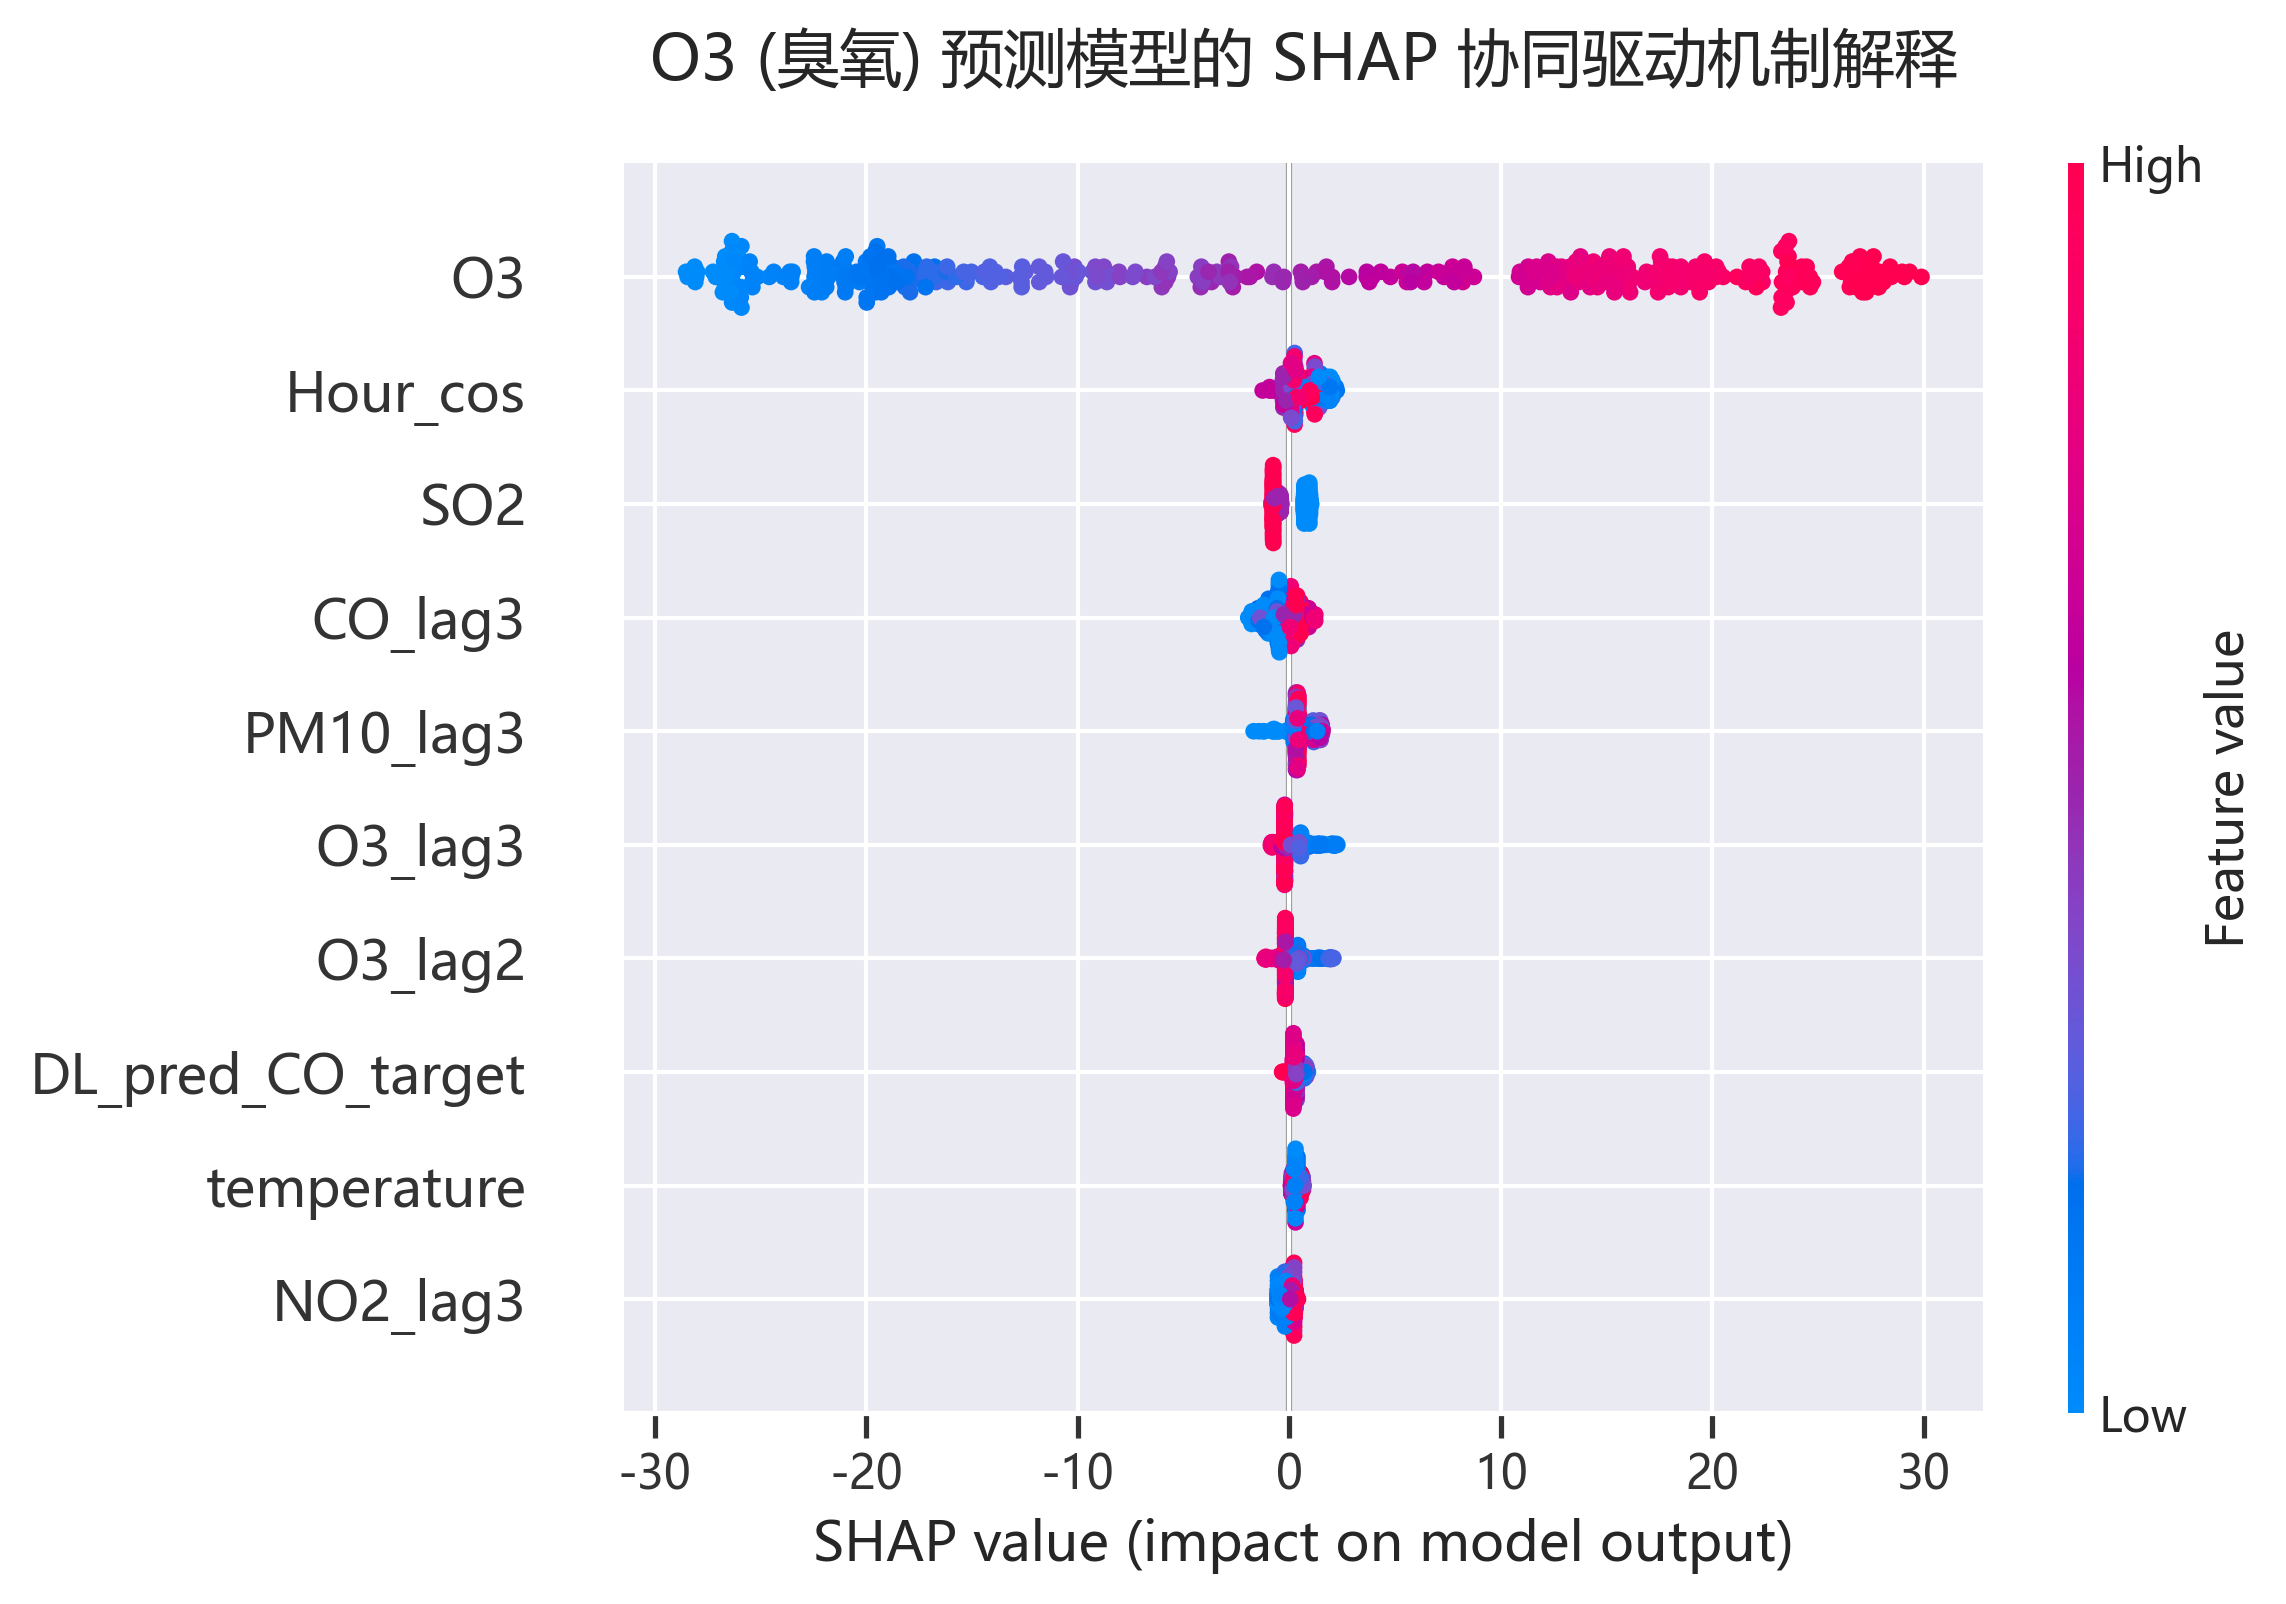
\includegraphics[width=\textwidth]{images/shap_o3.png}
        \caption{$\text{O}_3$ 协同驱动机制 SHAP 图}
        \label{fig:shap_o3}
    \end{subfigure}
    
    \caption{基于 SHAP 归因理论的污染物协同演化机制分析}
    \label{fig:total_shap_analysis}
\end{figure}

\textbf{（1）气态前体物向二次颗粒物的正向催化（协同富集效应）}

观察 $\text{PM}_{2.5}$ 的 SHAP 蜂群图可知，除自身浓度的时序惯性特征外，$\text{NO}_2$ 成为驱动其浓度生成的关键外部特征。图中 $\text{NO}_2$ 的红色散点（代表高特征值）显著聚集于 $\text{SHAP} > 0$ 的正半轴区域，这表明 \textbf{高浓度的 $\text{NO}_2$ 会强烈正向推动下一时刻 $\text{PM}_{2.5}$ 浓度的飙升}。

从大气化学机理视角审视，机动车尾气排放的氮氧化物（$\text{NO}_x$）在适宜的大气环境下极易转化为硝酸盐气溶胶，是二次细颗粒物生成的关键前体物。

\textbf{（2）温湿交互特征的“吸湿增长”驱动效应}

在 $\text{PM}_{2.5}$ 的解释模型中，本文构造的“温湿度交互项”表现出明显的右侧红点聚集现象。这定量化地证实了在相对温暖且高湿度的环境下，大气中的气溶胶粒子极易发生 \textbf{吸湿增长 (Hygroscopic Growth)}，导致细颗粒物质量浓度迅速攀升，进一步验证了复合气象条件对重污染天气的助推作用。

\textbf{（3）一次污染物与臭氧的“拮抗与光化学滴定”效应}

对 $\text{O}_3$ 的 SHAP 分析揭示了与颗粒物截然不同的驱动逻辑：
\begin{itemize}[itemsep=0pt, parsep=0pt]
    \item \textbf{热动力学催化：} 气温（\textit{temperature}）高值（红点）明显指向 SHAP 正值区，有力证实了光照辐射与高温是催化挥发性有机物（VOCs）生成臭氧的核心动力。
    \item \textbf{拮抗与滴定作用：} 观察发现一次污染物（如 $\text{CO}_{\text{lag3}}$、$\text{SO}_2$）的高浓度散点全部集中于 SHAP 负半轴。这深刻揭示了大气化学中的拮抗效应：当一次污染物浓度极高时（常对应夜间、冬季逆温层或低边界层环境），由于缺乏光照辅助，$\text{O}_3$ 无法有效合成；同时，高浓度的一氧化氮等会通过滴定反应迅速消耗现存臭氧，导致其 SHAP 贡献值为负。
\end{itemize}


\bigskip
\subsection{问题三：预测模型与基于国家标准的空气质量分级模型}

\subsubsection{空气质量分级映射模型的建立}
为了向校区学生提供直观、科学的空气质量评价与健康活动参考，国家生态环境部发布的《环境空气质量指数（AQI）技术规定（试行）》（HJ 633-2012）\cite{tech}与《环境空气质量标准》（GB 3095-2012）\cite{standard}，建立了空气质量分级映射模型。该模型主要分为以下三个计算步骤：

\textbf{（1）单项空气质量指数 (IAQI) 的计算}

由于不同污染物的量纲和对人体的危害阈值存在差异，本文首先采用分段线性插值法，将第 $p$ 种污染物的预测浓度值 $C_p$ 转化为无量纲的单项空气质量指数 $IAQI_p$。其数学计算公式如下：

\begin{equation}
IAQI_p = \frac{IAQI_{Hi} - IAQI_{Lo}}{BP_{Hi} - BP_{Lo}} (C_p - BP_{Lo}) + IAQI_{Lo}
\end{equation}

式中各参数含义如下：
\begin{itemize}
    \item $C_p$：第 $p$ 种污染物的预测质量浓度。本文涉及的单项污染物包括 $\text{PM}_{2.5}, \text{PM}_{10}, \text{O}_3, \text{NO}_2, \text{SO}_2, \text{CO}$。
    \item $BP_{Hi}, BP_{Lo}$：分别为《技术规定》查算表中与 $C_p$ 相近的污染物浓度限值的高位值与低位值。
    \item $IAQI_{Hi}, IAQI_{Lo}$：分别为对应于 $BP_{Hi}$ 与 $BP_{Lo}$ 的单项空气质量指数。
\end{itemize}

\textbf{（2）综合空气质量指数 (AQI) 与首要污染物的确定}

在求得上述 6 种污染物的 $IAQI$ 后，取其中的最大值作为该时刻的综合空气质量指数（AQI）：
\begin{equation}
AQI = \max \{IAQI_{\text{PM}2.5}, IAQI_{\text{PM}10}, IAQI_{\text{O}3}, IAQI_{\text{NO}2}, IAQI_{\text{SO}2}, IAQI_{\text{CO}}\}
\end{equation}

当 $AQI > 50$ 时，将 $IAQI$ 最大的单项污染物确定为该时刻的首要污染物。若有多种污染物的 $IAQI$ 并列最大，则均视为首要污染物。首要污染物的确定对于后续针对性地指导学生进行健康防护（如防颗粒物或防臭氧）具有关键的决策作用。

\textbf{（3）空气质量等级划分}

根据计算得出的综合 AQI 数值，将空气质量划分为 6 个等级。
\begin{table}[htbp]
\centering
\caption{空气质量指数 (AQI) 分级标准表}
\label{tab:aqi_standard}
\hspace*{-1.2cm}
% 将这里的 cccl 改为 cccc
\begin{tabular}{cccc}
\hline
\textbf{AQI 数值区间} & \textbf{空气质量等级} & \textbf{类别} & \textbf{对健康的影响推测} \\ \hline
0 $\sim$ 50 & 一级 & 优 & 空气质量令人满意，基本无空气污染 \\
51 $\sim$ 100 & 二级 & 良 & 极少数异常敏感人群应减少户外活动 \\
101 $\sim$ 150 & 三级 & 轻度污染 & 易感人群症状有轻度加剧，健康人群出现刺激症状 \\
151 $\sim$ 200 & 四级 & 中度污染 & 进一步加剧易感人群症状，对心脏、呼吸系统有影响 \\
201 $\sim$ 300 & 五级 & 重度污染 & 心肺病患者症状显著加剧，健康人群普遍出现症状 \\
> 300 & 六级 & 严重污染 & 健康人群运动耐受力降低，有明显强烈症状 \\ \hline
\end{tabular}
\end{table}

通过上述分级模型，本文将连续的污染物浓度预测序列映射为离散的、具有明确健康指导意义的等级标签，为后续的校园活动建议奠定了数据基础。

\subsubsection{基于多维环境感知矩阵的校园健康生活决策模型}

单纯的 AQI 等级只能反映空气污染的绝对程度，但在实际校园生活中，\textbf{温度与湿度同样极大地影响着人体舒适度以及污染物的毒理作用表现}。结合前文分析得出的结论，如高温对 $O_3$ 生成具有显著催化作用，以及高湿环境易促使颗粒物吸湿增长，本文综合“预测 AQI 等级”、“首要污染物”、“温度”与“湿度”四个维度，构建了良乡\textbf{校区健康生活决策矩阵 (Campus Health Life Decision Matrix)}。

针对良乡校区大学生的作息规律，模型设定了动态的指导规则，具体决策逻辑如表 \ref{tab:decision_matrix} 所示：

\begin{table}[h]
\centering
\renewcommand{\arraystretch}{1.5} 
\caption{良乡校区多维环境与健康生活决策矩阵}
\label{tab:decision_matrix}
% 优化后的列宽分配：
% 第一列从 2.2cm -> 2.8cm (撑开空间)
% 最后一列从 6.2cm -> 5.6cm (让出空间)
\begin{tabular}{|>{\centering\arraybackslash}m{2.8cm}|>{\centering\arraybackslash}m{2.0cm}|>{\centering\arraybackslash}m{3.5cm}|m{5.6cm}|}
\hline
\textbf{AQI 等级} & \textbf{首要污染物} & \textbf{气象条件触发器} & \multicolumn{1}{c|}{\textbf{面向良乡校区的活动指导建议}} \\ \hline
\textbf{优 / 良} \par (AQI $\le$ 100) & 无 或 任意 & $15^\circ\text{C} \le T \le 25^\circ\text{C}$ \par $30\% \le H \le 60\%$ & \textbf{[最佳活动期]} 强烈建议在操场/北湖进行晨跑、体测等剧烈有氧运动；建议宿舍全天开窗通风。 \\ \hline
\textbf{优 / 良} \par (AQI $\le$ 100) & $O_3$ (臭氧) & 气温 $T > 28^\circ\text{C}$ & \textbf{[防晒防臭氧]} 臭氧具有隐蔽性。13:00--16:00 尽量避免在缺乏遮挡的良乡中轴路长距离徒步；下午体育课建议转移至室内体育馆。 \\ \hline
\textbf{轻度 / 中度} \par (AQI 101$\sim$200) & $PM_{2.5}$ / $PM_{10}$ & 湿度 $H > 70\%$ & \textbf{[适度防护]} 停止高耗氧的室外长跑；前往文教/理教上课建议佩戴一次性医用口罩；早晚高峰宿舍不宜开窗。 \\ \hline
\textbf{轻度 / 中度} \par (AQI 101$\sim$200) & $NO_2$ / $SO_2$ / $CO$ & 气温 $T < 10^\circ\text{C}$ \par (常伴随早晚时段) & \textbf{[防范前体物]} 减少在交通干道（如良乡东路）周边的逗留时间，防止吸入机动车尾气；不建议晨跑。 \\ \hline
\textbf{重度 / 严重} \par (AQI > 200) & 颗粒物为主 & 任何温湿度条件 & \textbf{[红色警戒]} 停止一切户外社团活动和露天体育课；外出必须佩戴 N95/KN95 口罩；宿舍严禁开窗，建议开启空气净化器。 \\ \hline
\end{tabular}
\end{table}

通过该决策矩阵，本模型成功将复杂的“环境--气象”多变量时序预测结果，转化为同学们通俗易懂的\textbf{每日校园生活行动指南}。


% ==================== 第五部分：模型结果分析 ====================
\section{模型结果分析}

本节对所建立的BiLSTM+XGBoost级联融合模型在多污染物协同预测任务中的表现进行系统分析，并结合特征重要性与可解释性方法，深入探讨模型的物理意义与实际应用价值。

\subsection{预测精度与拟合效果评估}
如表~\ref{tab:evaluation_results}所示，模型在测试集上对六种主要污染物的预测均取得了较高的拟合精度。$R^2$决定系数普遍高于0.84，SO$_2$、CO等污染物的$R^2$甚至超过0.98，表明模型能够有效捕捉污染物的时序演化规律。图~\ref{fig:prediction_tracking}进一步展示了模型对未来120小时污染物浓度的追踪预测，预测曲线与真实观测值高度吻合，能够准确反映早晚高峰的污染物峰值及午后低谷，验证了模型的时序外推能力和协同演化捕捉能力。

\subsection{特征重要性与物理机制解读}
通过XGBoost特征重要性热力图（见图~\ref{fig:importance_heatmap}），可以发现：
\begin{itemize}
    \item 污染物自身的历史浓度（如$SO_{2\_lag1}$、$CO_{lag1}$）对未来预测具有最强驱动作用，体现了空气质量的时序惯性；
    \item $NO_2$作为前体物，对$PM_{2.5}$、$PM_{10}$等颗粒物的预测贡献显著，符合机动车尾气促进二次颗粒物生成的物理机制；
    \item 温度、湿度等气象因子的滞后特征在多污染物预测中同样占据重要地位，反映了气象条件对污染物累积与消散的长效影响。
\end{itemize}


\begin{spacing}{1}
\bigskip
\section{总结}
\subsection{模型可解释性与协同变化规律}
基于SHAP归因分析（见图~\ref{fig:total_shap_analysis}），模型自动提取出以下协同演化机制：
\begin{itemize}
    \item $NO_2$高值显著正向推动$PM_{2.5}$浓度，验证了气态前体物向二次颗粒物的催化效应；
    \item 温湿度交互项对颗粒物有正向促进作用，体现了高温高湿环境下的吸湿增长现象；
    \item 一次污染物（如CO、SO$_2$）高值对O$_3$有负向抑制作用，揭示了光化学滴定和拮抗效应。
\end{itemize}
这些结论与大气物理化学理论高度一致，说明模型不仅具备良好的预测能力，还能为污染物协同变化的机理研究提供数据支持。

\subsection{模型局限性与改进方向}
尽管模型在测试集上表现优异，但仍存在以下局限：
\begin{itemize}
    \item 仅选取温度、湿度等有限气象因子，未考虑风速、气压等潜在影响因素；
    \item 滞后特征的选取基于经验，未来可引入自动特征选择或更复杂的时序建模方法；
    \item 极端天气或突发事件下的预测能力有待进一步验证。
\end{itemize}
后续可通过引入更多气象变量、优化特征工程、融合外部数据等方式进一步提升模型的泛化能力和物理解释力。

\end{spacing}

% ==================== 结果分析结束 ====================
\section{参考文献}
\renewcommand{\refname}{} 
\vspace{-3.5em} 
\begin{thebibliography}{99}

\bibitem{fan2012} 范明, 孟小峰. 数据挖掘概念与技术(第3版)[M]. 北京: 机械工业出版社, 2012: 56-59.

\bibitem{spearman1904} Spearman C. The proof and measurement of association between two things[J]. The American Journal of Psychology, 1904, 15(1): 72-101.

\bibitem{tech} 中华人民共和国环境保护部. 环境空气质量指数（AQI）技术规定（试行）: HJ 633-2012[S]. 北京: 中国环境科学出版社, 2012.

\bibitem{standard} 中华人民共和国环境保护部, 国家质量监督检验检疫总局. 环境空气质量标准: GB 3095-2012[S]. 北京: 中国环境科学出版社, 2012.

\bibitem{bilstm} GRAVES A, SCHMIDHUBER J. Framewise phoneme classification with bidirectional LSTM and other network architectures[J]. Neural Networks, 2005, 18(5-6): 602-610.

\bibitem{xgboost} CHEN T, GUESTURIN C. XGBoost: A scalable tree boosting system[C]//Proceedings of the 22nd ACM SIGKDD International Conference on Knowledge Discovery and Data Mining. New York: ACM, 2016: 785-794.
\end{thebibliography}

\section{人工智能工具使用报告}
在本篇论文的撰写过程中，本参赛队使用了生成式人工智能工具 \textbf{Gemini 3.1 pro}。本队严格遵守竞赛规则，仅将 AI 工具用于辅助文献理解与格式校验，现将具体使用情况报告如下：
\subsection{问题一}
\begin{itemize}[itemsep=0pt, parsep=0pt]
    \item \textbf{提示词 (Prompt) ：} “请阅读附件材料，解释一下良乡地区 $O_3$ 浓度在夜间出现低谷的‘滴定效应’具体指什么化学反应？同时总结湿度对颗粒物‘吸湿增长’影响的物理逻辑。”
    \item \textbf{AI 生成内容：} AI 基于背景材料，准确提取了 $NO + O_3 \rightarrow NO_2 + O_2$ 的滴定反应逻辑，并解释了气溶胶粒子在高湿环境下物理粒径增大的机理。
\end{itemize}

\subsection{问题二}
\begin{itemize}[itemsep=0pt, parsep=0pt]
    \item \textbf{提示词 (Prompt) ：} “我编写了一个包含 \texttt{tabularx} 环境的表格，但在编译时报错‘Undefined control sequence’，请帮我检查是否漏掉宏包，并优化该表格的垂直居中代码。”
    \item \textbf{AI 生成内容：} AI 指出本队遗漏了 \texttt{array} 宏包，并提供了基于 \texttt{m\{width\}} 格式的垂直居中优化建议。
\end{itemize}

\newpage
\section{附录}
\subsection{支撑文件列表}
按照竞赛规则第十条要求，本团队已将建模所用的可运行源程序、自主查阅的拓展参考文献以及较大篇幅的高清图表打包压缩为 \texttt{ZIP} 附件。各文件组织结构及功能说明如下：

\vspace{1em} % 增加一点垂直间距

\dirtree{%
.1 支撑材料.zip.
.2 src/ \quad (核心可运行源程序).
.3 1.py \quad (问题一：24h浓度变化/Spearman).
.3 2.py \quad (问题二：BiLSTM + XGBoost模型代码).
.3 3.py \quad (问题三：AQI污染物计算).
.2 graphy/ \quad (大篇幅中间结果与高清图表).
.3 1/ \quad (问题一相关图表：包含24h浓度变化图等).
.3 2/ \quad (问题二相关图表：SHAP蜂腰图等).
.3 3/ \quad (问题三相关图表：良乡校区多维环境与健康生活决策矩阵等).
.2 参考文献/ \quad (自主查阅的外部算法论文与文献，非赛题给出).
.3 1904-spearman.pdf.
.2 main.tex \quad (本论文的 \LaTeX 源文件).
}

\vspace{1em}
\noindent\textbf{运行环境说明：} 
所有 \texttt{.py} 源代码均基于 Python 3.8 编写，核心依赖库包括 \texttt{pandas}, \texttt{numpy}, \texttt{scikit-learn}, \texttt{xgboost}, \texttt{shap} 等。评审专家可直接运行 \texttt{src/} 目录下的脚本复现本论文的全部结论与图表。

\newpage
\subsection{图表汇总}
\bigskip
% 图1
\begin{figure}[htbp]
    \centering
    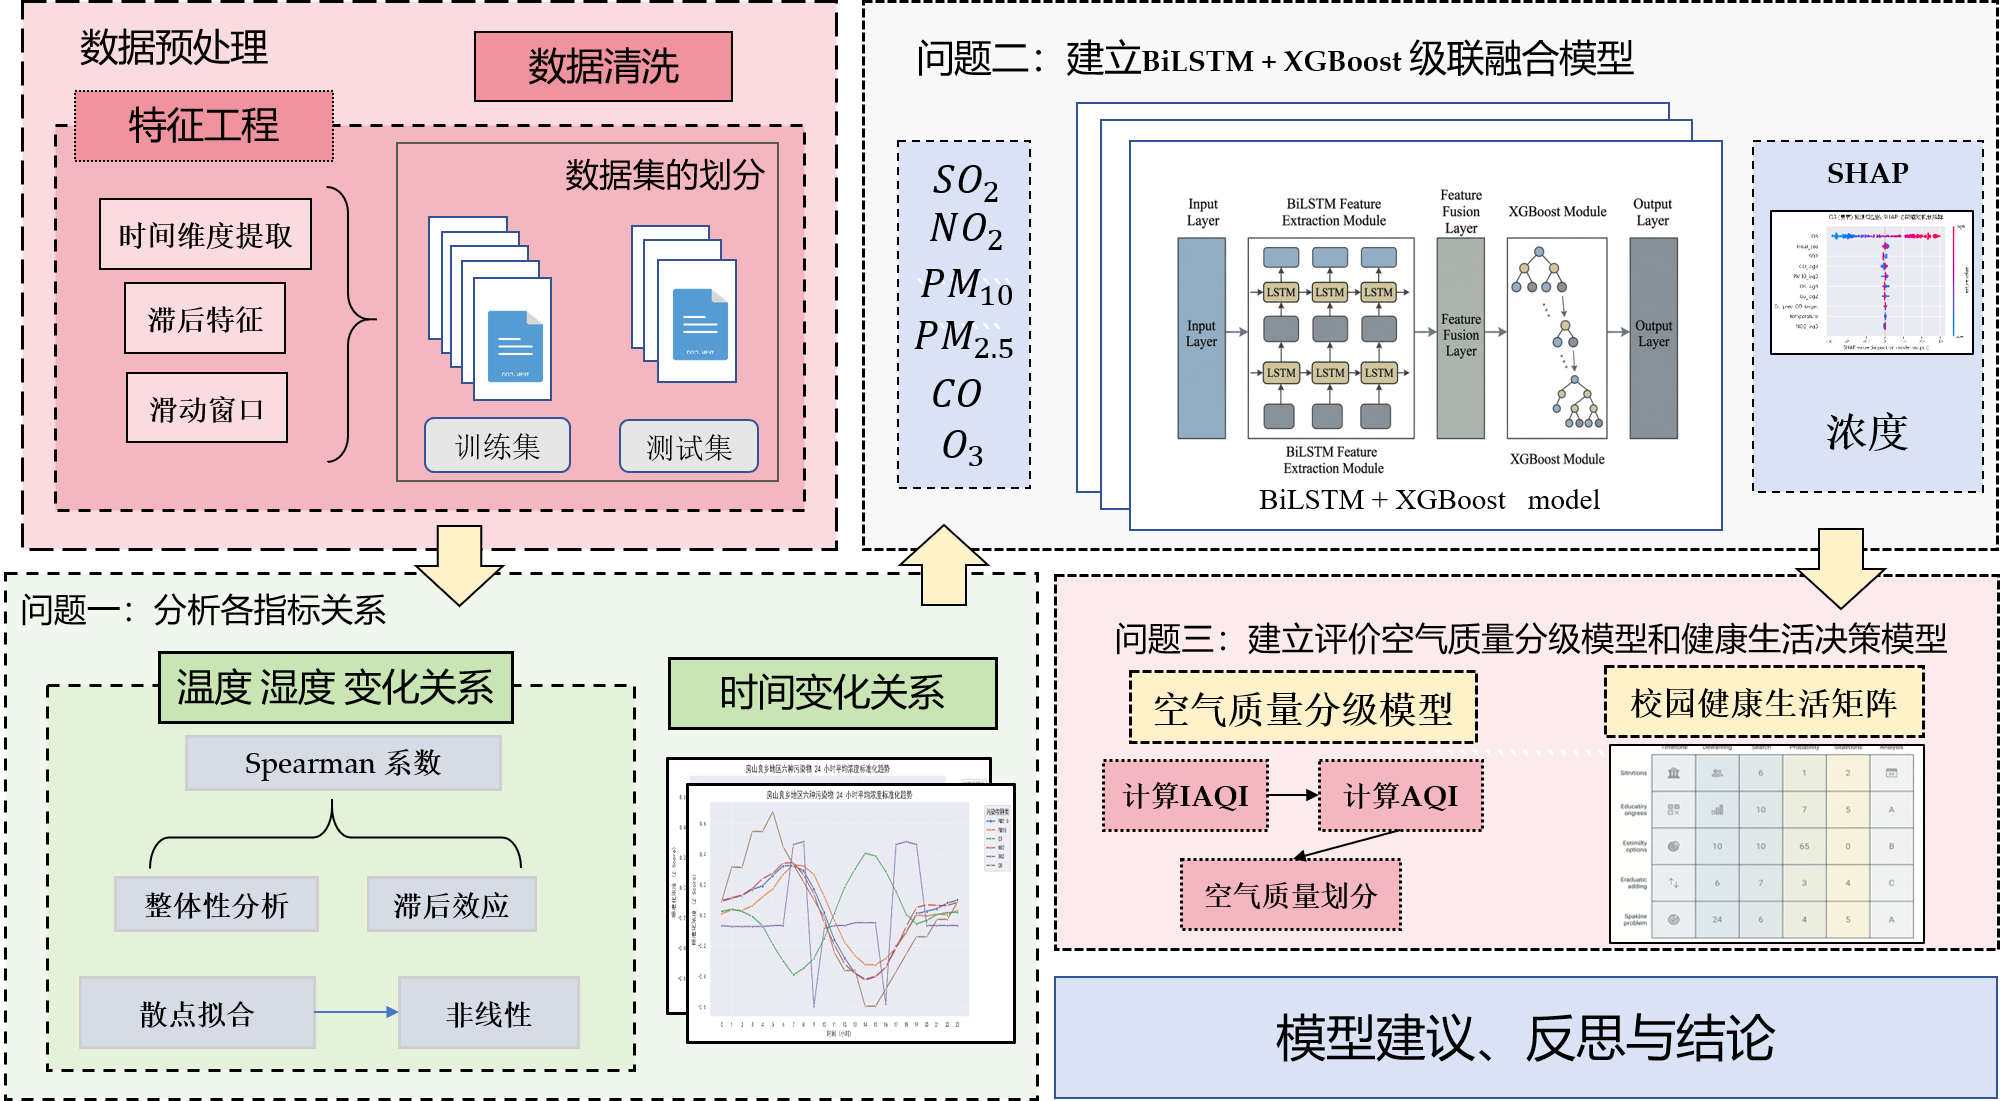
\includegraphics[width=1.1\textwidth]{images/thinking.png} 
    \caption{BiLSTM + XGBoost 级联融合模型示意图}
    \label{fig:summary-idea}
\end{figure}
\bigskip
% 图2
\begin{figure}[htbp]
    \centering
    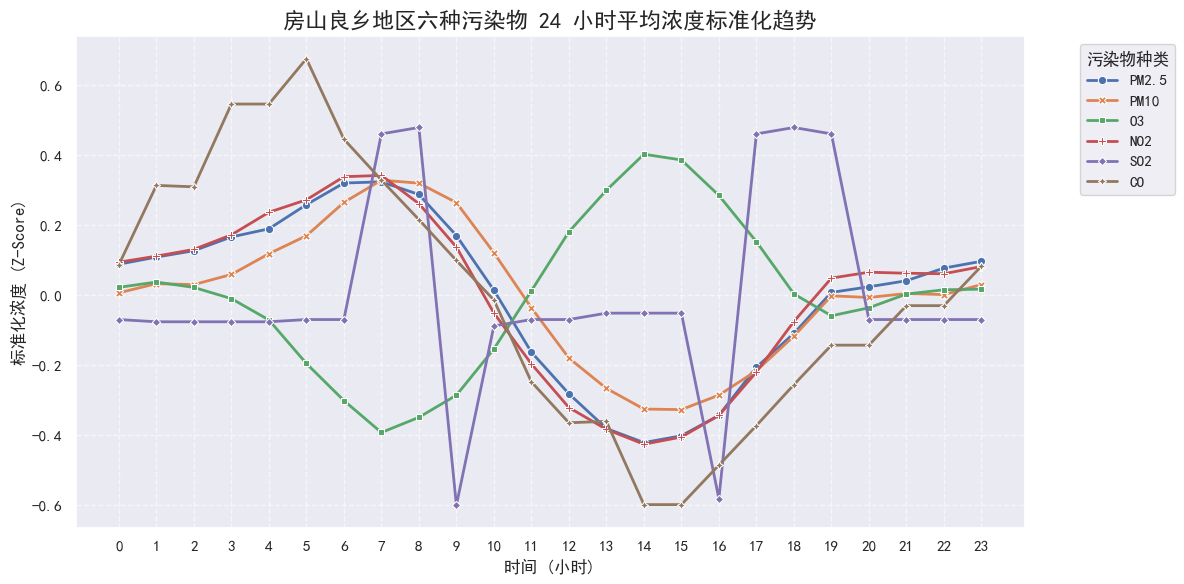
\includegraphics[width=1.1\textwidth]{images/1.png} 
    \caption{良乡地区六种污染物 24 小时平均浓度趋势变化图}
    \label{fig:summary-24h-trend}
\end{figure}
\bigskip
% 图3
\begin{figure}[htbp]
    \centering
    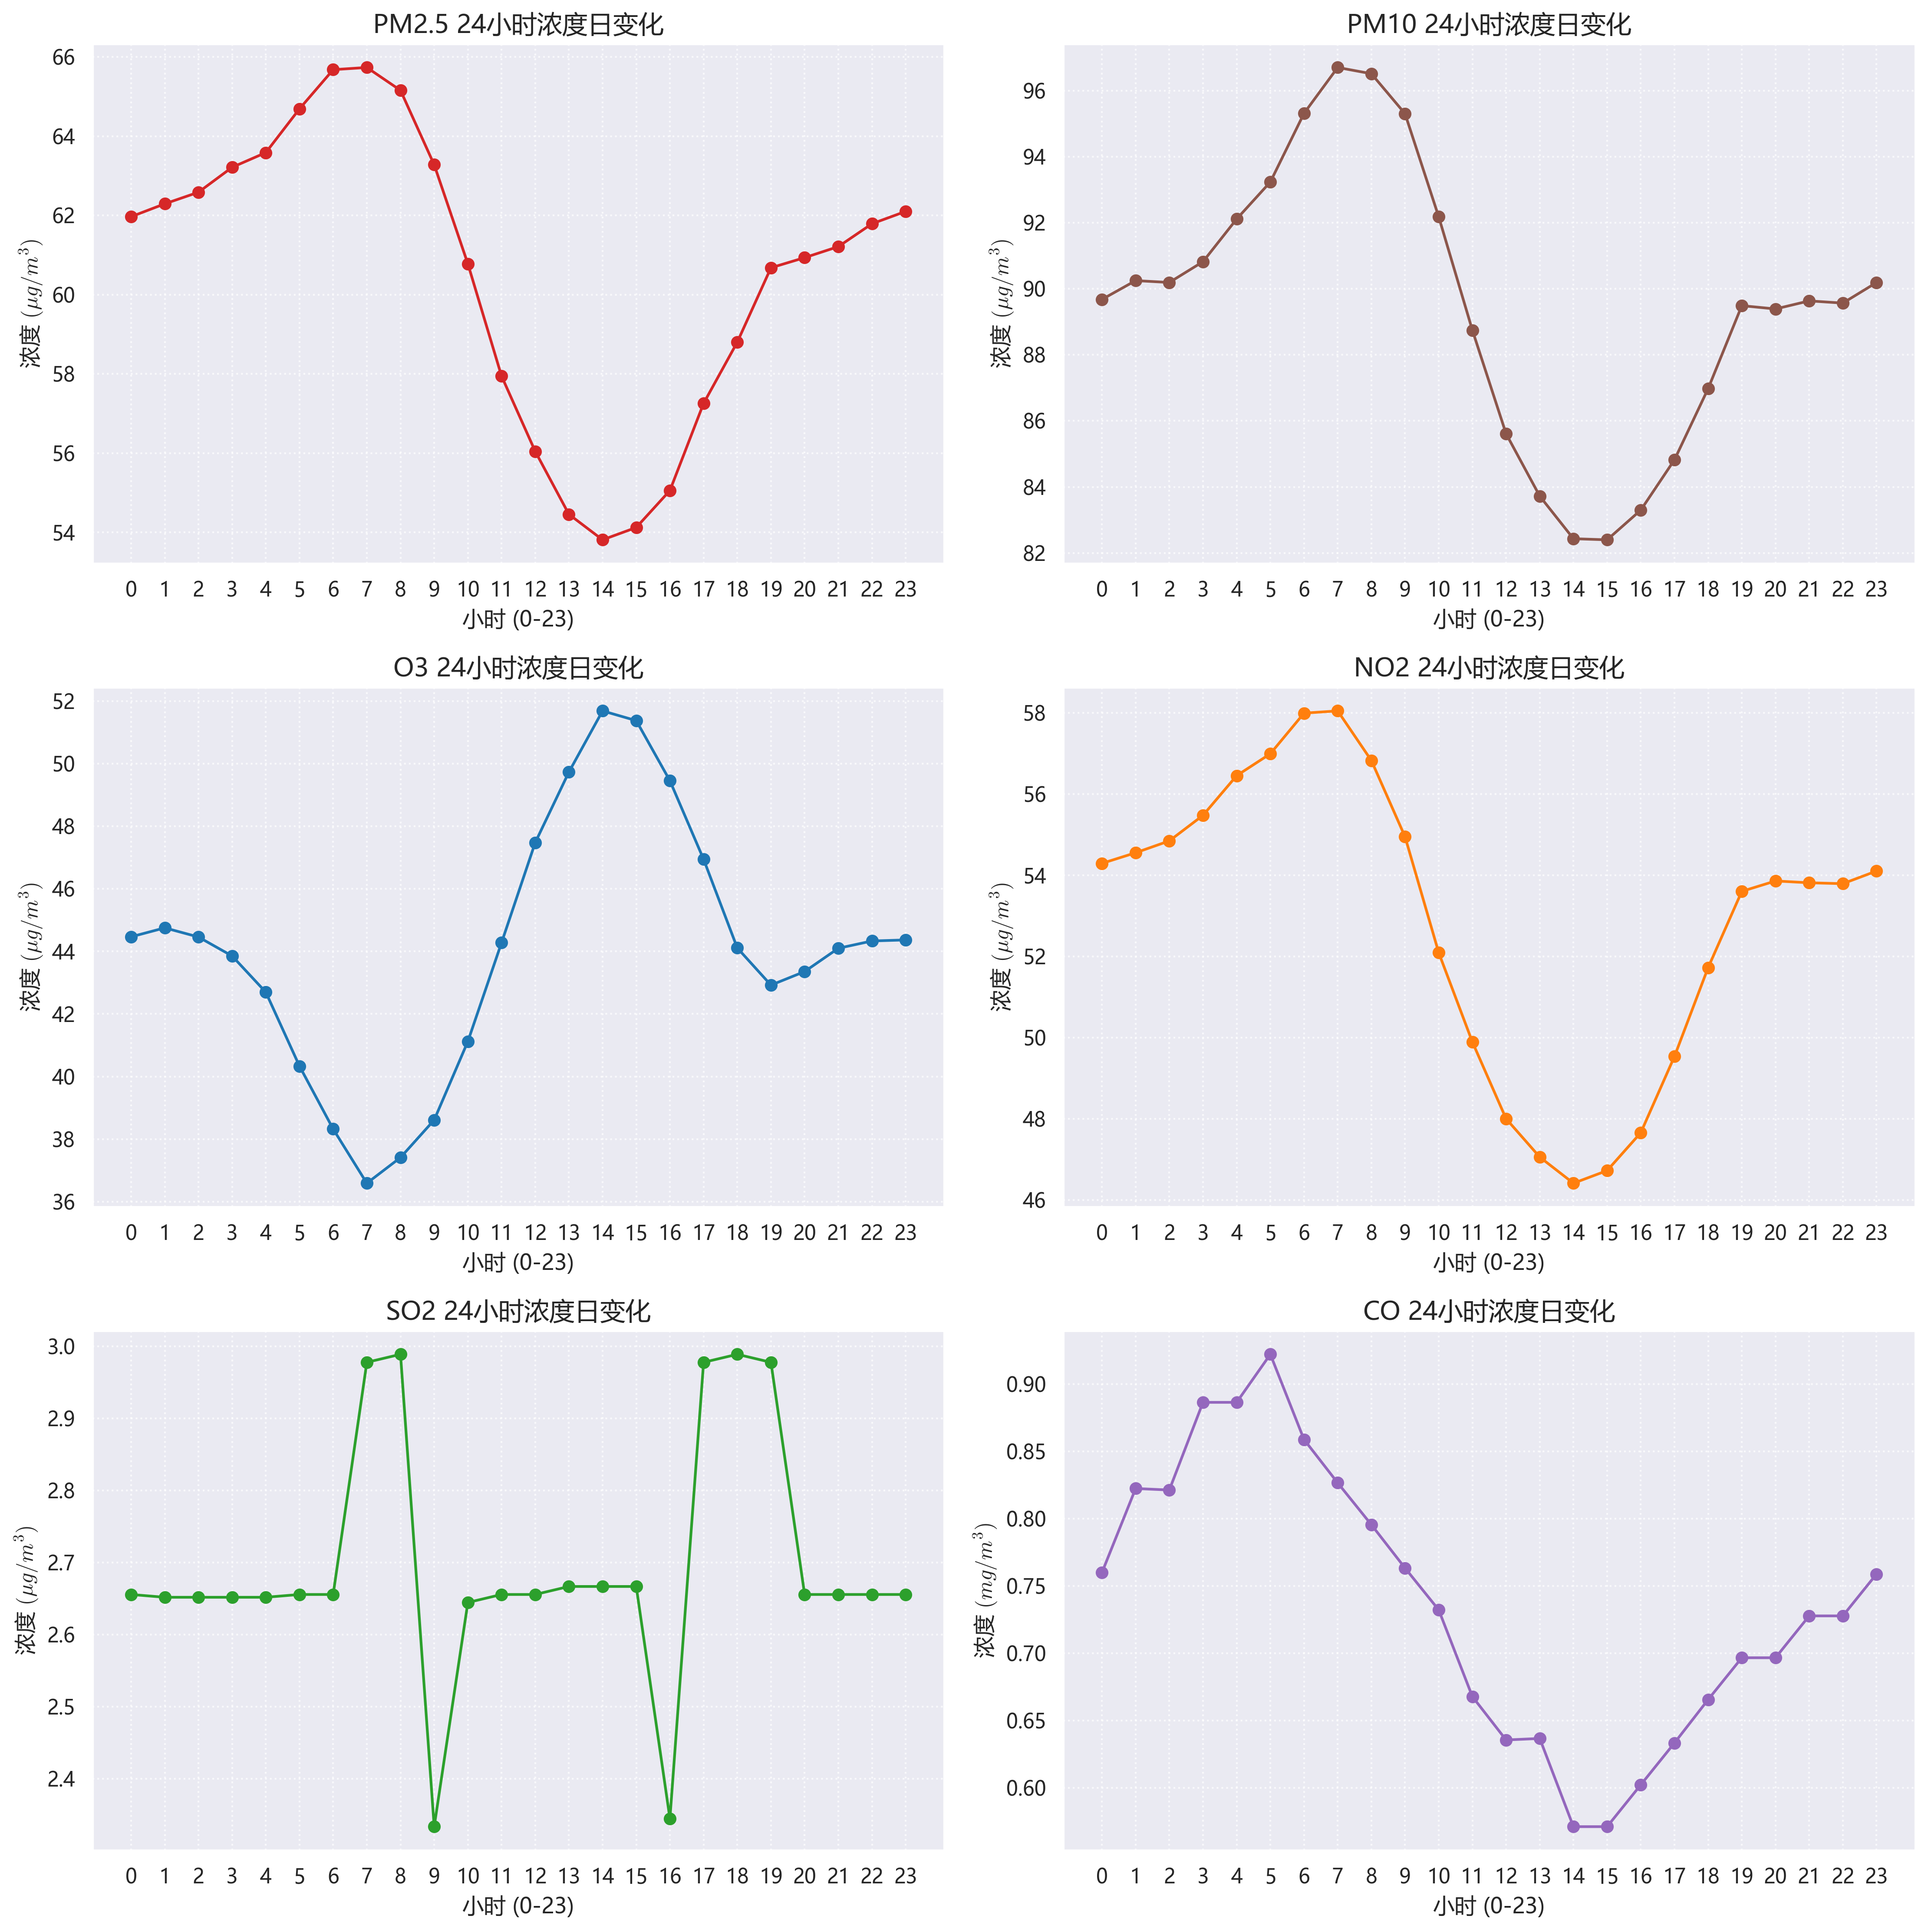
\includegraphics[width=1.2\textwidth]{images/2.png} 
    \caption{良乡地区六种污染物 24 小时浓度日变化图}
    \label{fig:summary-24h-daily}
\end{figure}
\bigskip
% 图4
\begin{figure}[htbp]
    \centering
    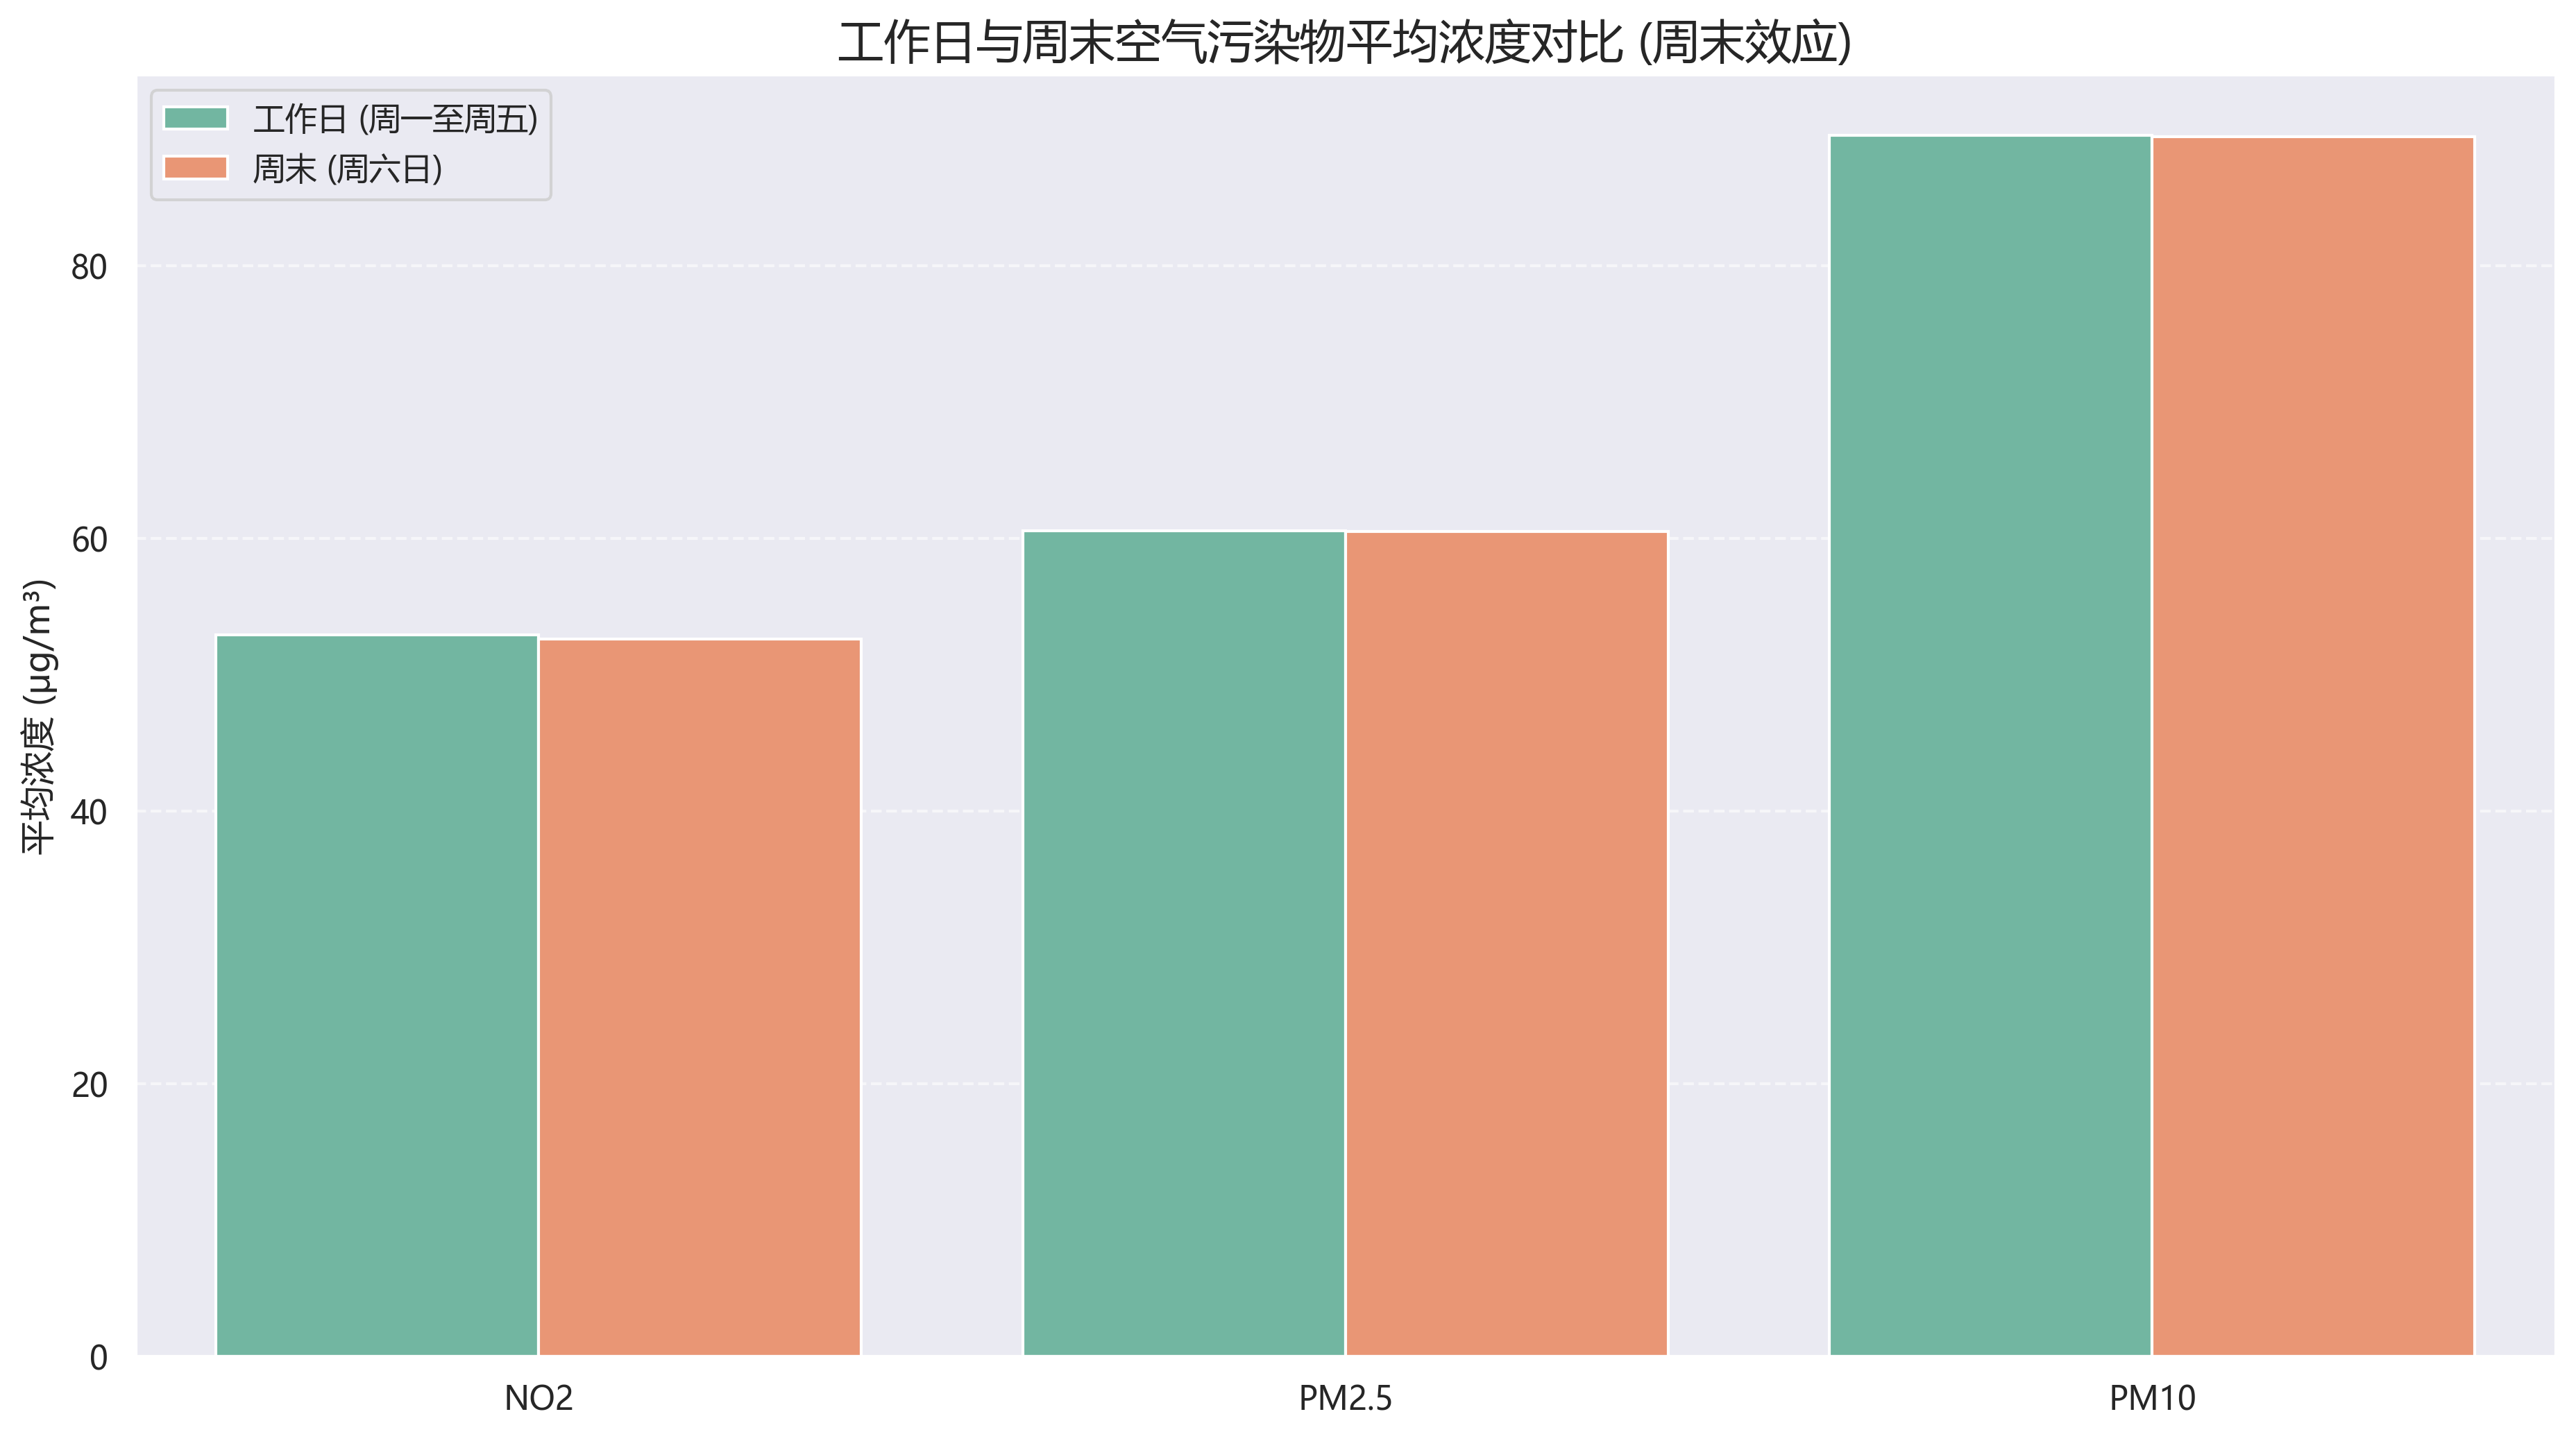
\includegraphics[width=0.9\textwidth]{images/3.png} 
    \caption{工作日与周末空气污染物平均浓度对比}
    \label{fig:summary-weekend}
\end{figure}
\bigskip
% 图5
\begin{figure}[htbp]
    \centering
    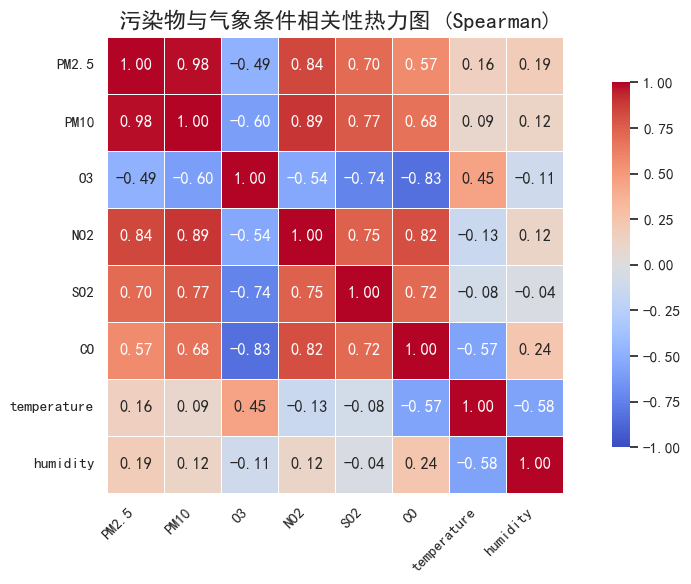
\includegraphics[width=0.8\textwidth]{images/5.png} 
    \caption{污染物与气象条件相关热力图}
    \label{fig:summary-corr}
\end{figure}
\bigskip
% 图6
\begin{figure}[htbp]
    \centering
    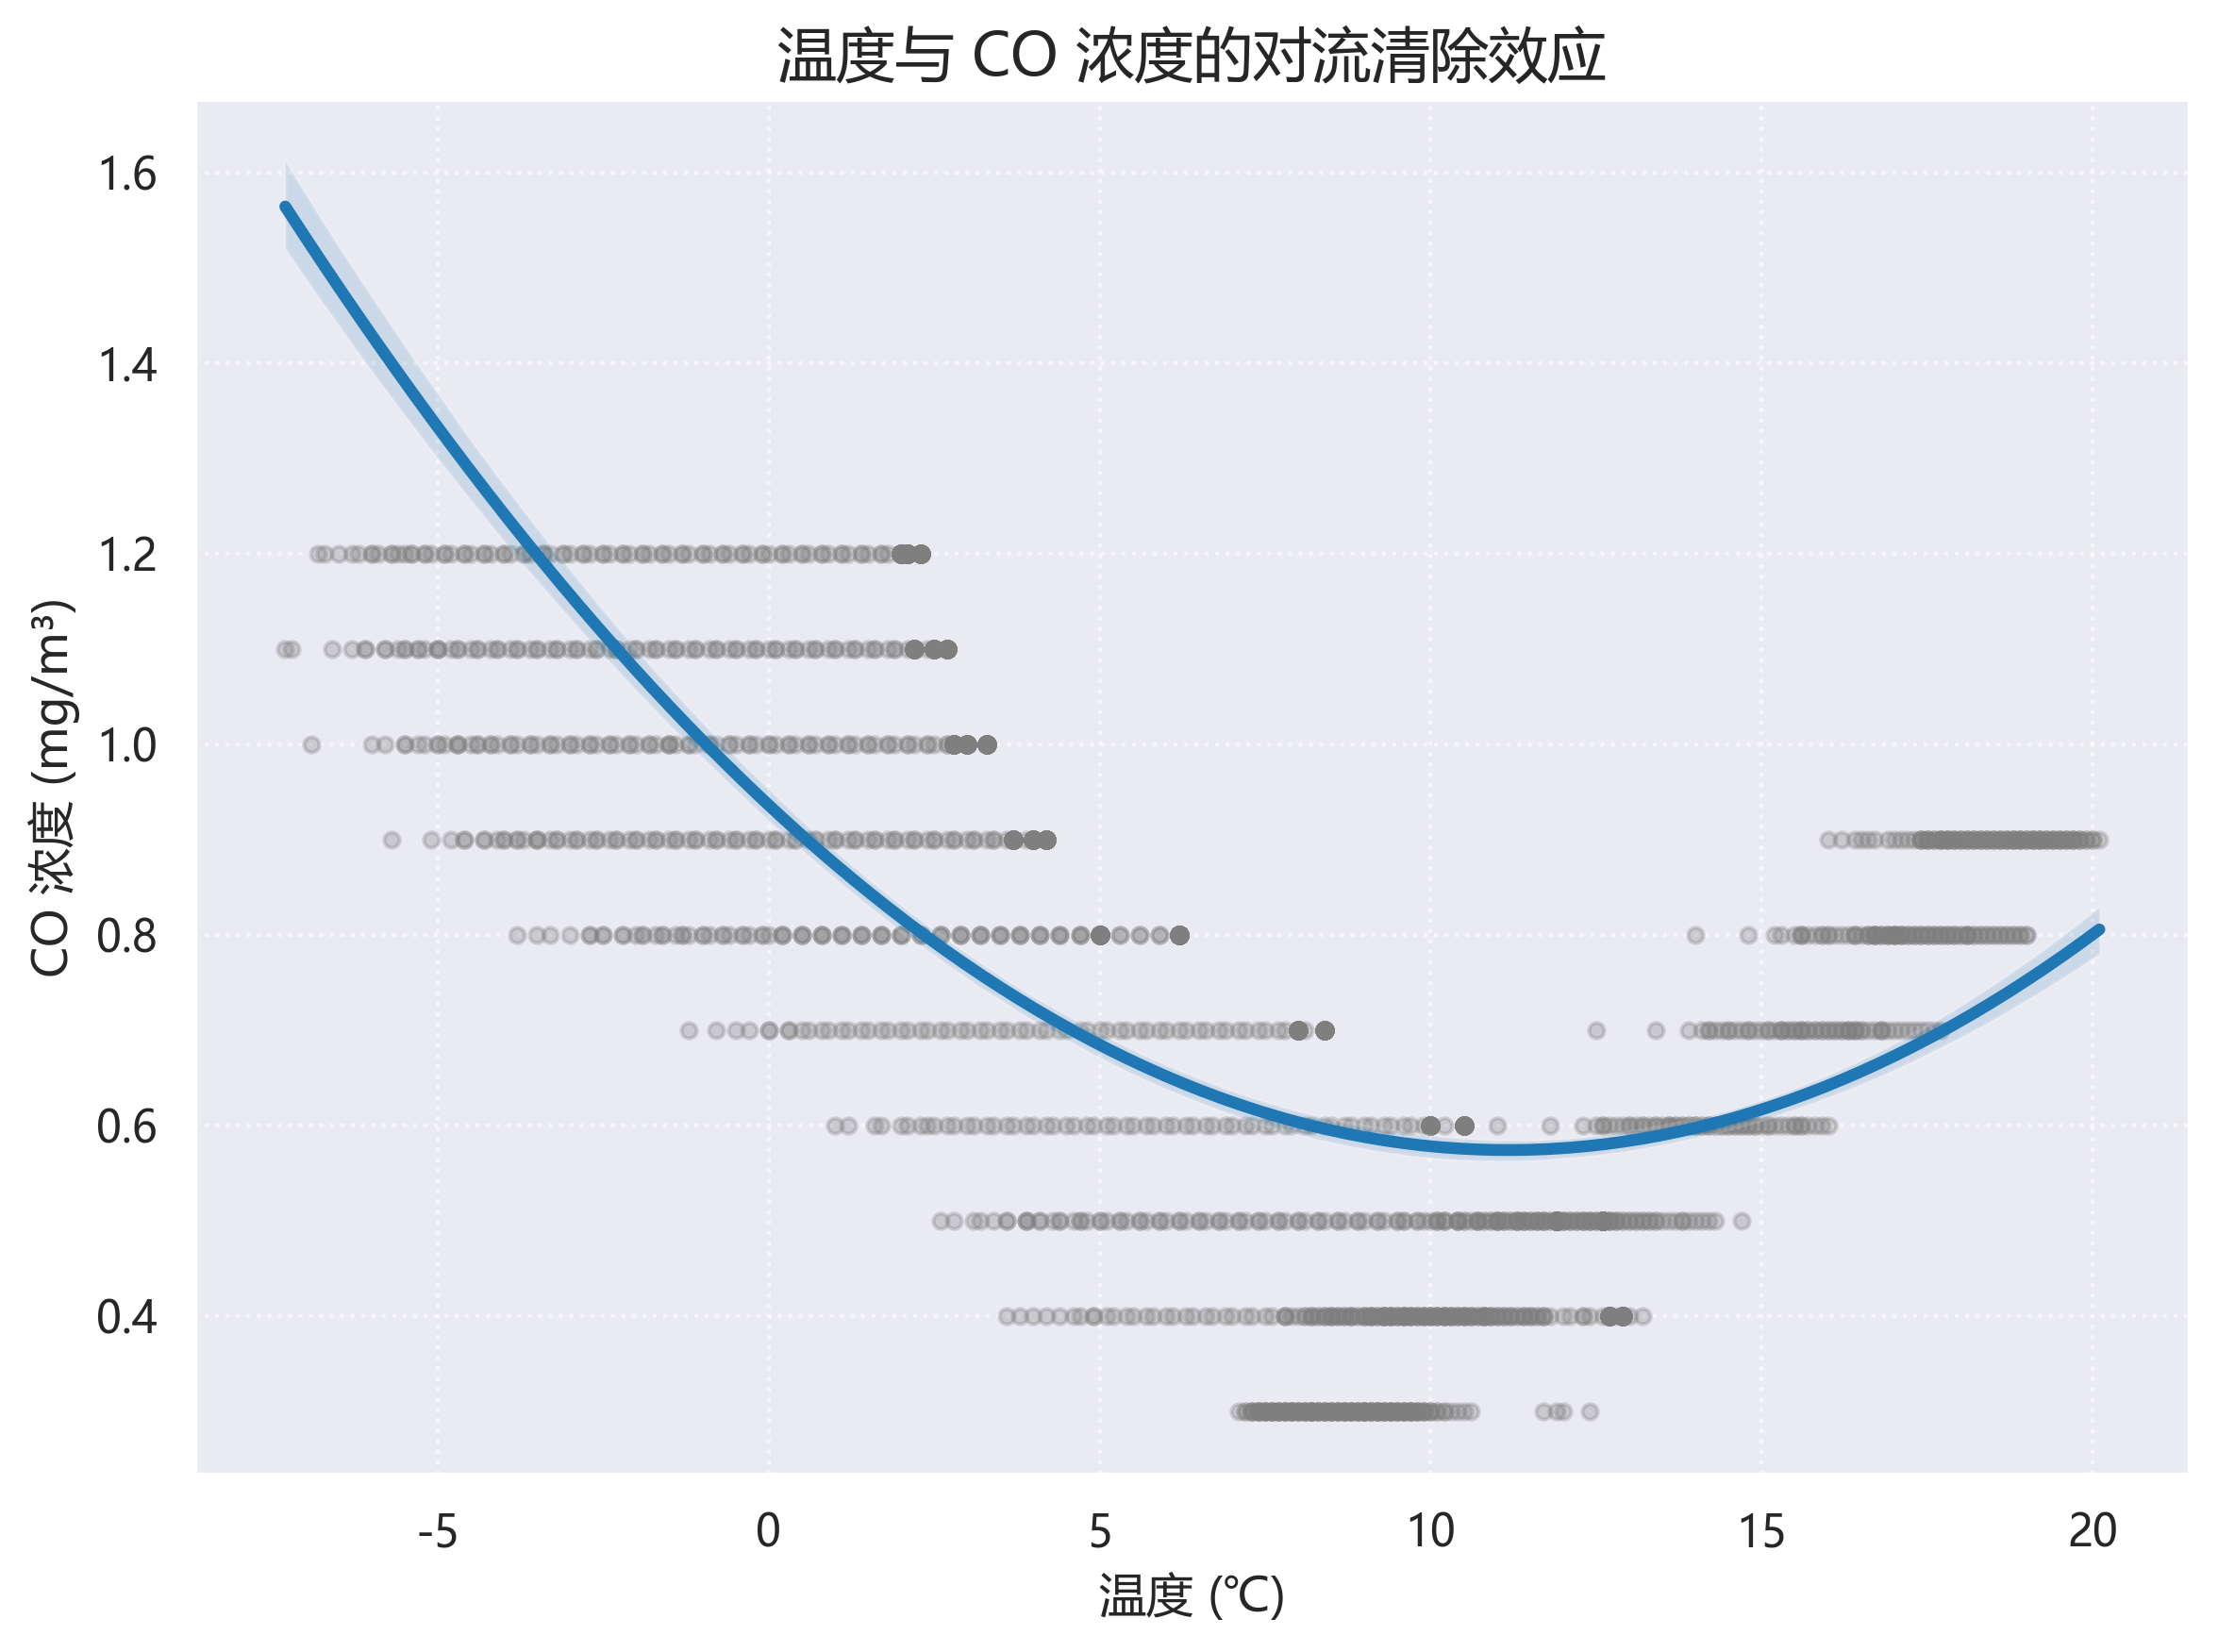
\includegraphics[width=0.8\textwidth]{images/6.png}
    \caption{温度与 $O_3$ 浓度的非线性响应关系}
    \label{fig:summary-temp-o3}
\end{figure}
\bigskip
% ...依次添加所有figure/table...

% 表1
\begin{table}[htbp]
    \centering
    \caption{BiLSTM-XGBoost 级联模型测试集评估结果}
    \label{tab:summary-evaluation}
    \begin{tabularx}{\textwidth}{@{} YYYY @{}} 
        \toprule
        \textbf{污染物} & \textbf{RMSE} & \textbf{MAE} & \textbf{$R^2$} \\
        \midrule
        $PM_{2.5}$ & 5.5239 & 3.8721 & 0.8439 \\
        $PM_{10}$  & 9.4016 & 6.8562 & 0.8452 \\
        $O_3$      & 3.6329 & 2.6966 & 0.9663 \\
        $NO_2$     & 2.1756 & 1.6005 & 0.9753 \\
        $SO_2$     & 0.0707 & 0.0359 & 0.9925 \\
        $CO$       & 0.0226 & 0.0146 & 0.9897 \\
        \bottomrule
    \end{tabularx}
\end{table}
\bigskip
% ...依次添加所有table...

\end{document}

